\documentclass[twoside]{book}

% Packages required by doxygen
\usepackage{fixltx2e}
\usepackage{calc}
\usepackage{doxygen}
\usepackage[export]{adjustbox} % also loads graphicx
\usepackage{graphicx}
\usepackage[utf8]{inputenc}
\usepackage{makeidx}
\usepackage{multicol}
\usepackage{multirow}
\PassOptionsToPackage{warn}{textcomp}
\usepackage{textcomp}
\usepackage[nointegrals]{wasysym}
\usepackage[table]{xcolor}

% Font selection
\usepackage[T1]{fontenc}
\usepackage[scaled=.90]{helvet}
\usepackage{courier}
\usepackage{amssymb}
\usepackage{sectsty}
\renewcommand{\familydefault}{\sfdefault}
\allsectionsfont{%
  \fontseries{bc}\selectfont%
  \color{darkgray}%
}
\renewcommand{\DoxyLabelFont}{%
  \fontseries{bc}\selectfont%
  \color{darkgray}%
}
\newcommand{\+}{\discretionary{\mbox{\scriptsize$\hookleftarrow$}}{}{}}

% Page & text layout
\usepackage{geometry}
\geometry{%
  a4paper,%
  top=2.5cm,%
  bottom=2.5cm,%
  left=2.5cm,%
  right=2.5cm%
}
\tolerance=750
\hfuzz=15pt
\hbadness=750
\setlength{\emergencystretch}{15pt}
\setlength{\parindent}{0cm}
\setlength{\parskip}{3ex plus 2ex minus 2ex}
\makeatletter
\renewcommand{\paragraph}{%
  \@startsection{paragraph}{4}{0ex}{-1.0ex}{1.0ex}{%
    \normalfont\normalsize\bfseries\SS@parafont%
  }%
}
\renewcommand{\subparagraph}{%
  \@startsection{subparagraph}{5}{0ex}{-1.0ex}{1.0ex}{%
    \normalfont\normalsize\bfseries\SS@subparafont%
  }%
}
\makeatother

% Headers & footers
\usepackage{fancyhdr}
\pagestyle{fancyplain}
\fancyhead[LE]{\fancyplain{}{\bfseries\thepage}}
\fancyhead[CE]{\fancyplain{}{}}
\fancyhead[RE]{\fancyplain{}{\bfseries\leftmark}}
\fancyhead[LO]{\fancyplain{}{\bfseries\rightmark}}
\fancyhead[CO]{\fancyplain{}{}}
\fancyhead[RO]{\fancyplain{}{\bfseries\thepage}}
\fancyfoot[LE]{\fancyplain{}{}}
\fancyfoot[CE]{\fancyplain{}{}}
\fancyfoot[RE]{\fancyplain{}{\bfseries\scriptsize Generated by Doxygen }}
\fancyfoot[LO]{\fancyplain{}{\bfseries\scriptsize Generated by Doxygen }}
\fancyfoot[CO]{\fancyplain{}{}}
\fancyfoot[RO]{\fancyplain{}{}}
\renewcommand{\footrulewidth}{0.4pt}
\renewcommand{\chaptermark}[1]{%
  \markboth{#1}{}%
}
\renewcommand{\sectionmark}[1]{%
  \markright{\thesection\ #1}%
}

% Indices & bibliography
\usepackage{natbib}
\usepackage[titles]{tocloft}
\setcounter{tocdepth}{3}
\setcounter{secnumdepth}{5}
\makeindex

% Packages requested by user
\usepackage{amsmath}
\usepackage{pgfplots[compat=1.9]}

% Hyperlinks (required, but should be loaded last)
\usepackage{ifpdf}
\ifpdf
  \usepackage[pdftex,pagebackref=true]{hyperref}
\else
  \usepackage[ps2pdf,pagebackref=true]{hyperref}
\fi
\hypersetup{%
  colorlinks=true,%
  linkcolor=blue,%
  citecolor=blue,%
  unicode%
}

% Custom commands
\newcommand{\clearemptydoublepage}{%
  \newpage{\pagestyle{empty}\cleardoublepage}%
}

\usepackage{caption}
\captionsetup{labelsep=space,justification=centering,font={bf},singlelinecheck=off,skip=4pt,position=top}

%===== C O N T E N T S =====

\begin{document}

% Titlepage & ToC
\hypersetup{pageanchor=false,
             bookmarksnumbered=true,
             pdfencoding=unicode
            }
\pagenumbering{roman}
\begin{titlepage}
\vspace*{7cm}
\begin{center}%
{\Large Echelle++ }\\
\vspace*{1cm}
{\large Generated by Doxygen 1.8.11}\\
\end{center}
\end{titlepage}
\clearemptydoublepage
\tableofcontents
\clearemptydoublepage
\pagenumbering{arabic}
\hypersetup{pageanchor=true}

%--- Begin generated contents ---
\chapter{Welcome to the Documentation of Echelle++}
\label{index}\hypertarget{index}{}This documentation is divided in the following sections\+:
\begin{DoxyItemize}
\item \hyperlink{intro}{Introduction}
\item \hyperlink{concept}{General concept}
\item \hyperlink{installation}{Installation}
\item \hyperlink{usage}{Usage}
\item Examples
\item Class documentation 
\end{DoxyItemize}
\chapter{Concept}
\label{concept}
\hypertarget{concept}{}
The basic idea is that for a specific wavelength, the response of the spectrograph to a certain input illumination can be described by a 3x3 transformation matrix and a subsequent convolution with a point spread function (\hyperlink{class_p_s_f}{P\+SF}). Both, the transformation matrices and the P\+S\+Fs are therefore wavelength dependent. It is reasonable to assume that along a single echelle order, the P\+S\+Fs and transformation parameters will vary smoothly. If we know the matrices and P\+S\+Fs for a sufficient large number of wavelength, we can interpolate between them for arbitrary wavelength.

\subsection*{Transformation matrices}

At a monochromatic wavelength, the information about the mapping of the input slit / fiber onto the detector of the spectrograph can be described by a 3x3 transformation matrix. In principle there are two geometric transformation we could choose from\+: Affine and projective transformation. While the latter is more general, we found that affine transformations are sufficiently accurate to describe the spectrograph optics. Affine transformation parameters also give an intuitive insight in what happens across an order, because they can be expressed in terms of rotation( $\Theta$), shear ( $shear$), scaling in both directions ( $sx$ and $sy$ ) and translation ( $tx$ and $ty$ ) .

There is no unique definition of how do compose an affine transformation matrix, we will use the following\+:

\[ M_{\lambda} = \begin{pmatrix} sx \cdot \cos(\Theta) & -sy \cdot \sin(\Theta+shear) & tx \\ sx \cdot \sin(\Theta) & sy \cdot \cos(\Theta+shear) & ty \\ 0 & 0 & 1 \end{pmatrix} \]

As an example, we plot the scale parameter in x-\/direction (dispersion direction) as a function of wavelength for the MaroonX spectrograph. Data of the same echelle order are connected by a line. The anamorphic magnification of the spectrograph is directly reflected by an increase of {\itshape sx} across each order. On the right plot we see {\itshape sx} for order 100. Note that the increase of {\itshape sx} with wavelength is not a linear, but a smooth function.



\subsection*{Point Spread Function}

While the transformation matrix describes well the coarse behaviour of a spectrograph at a specific wavelength, we need additional information to account for all optical aberrations that occur in a realistic spectrograph. The point spread function (or \hyperlink{class_p_s_f}{P\+SF}) is defined as the response of an optical system to a point source.

Casually speaking, the \hyperlink{class_p_s_f}{P\+SF} leads to a blur of the imaged input slit. In a spectrograph, this blur of the \hyperlink{class_p_s_f}{P\+SF} will usually be of the same size or smaller than the size of the input slit on the detector.

The shape of the \hyperlink{class_p_s_f}{P\+SF} can have a complex form, and using a simple Gaussian function might not accurately describe the \hyperlink{class_p_s_f}{P\+SF}. The \hyperlink{class_p_s_f}{P\+SF} will vary in form and size across the detector, depending on the subtleties of the optics for a specific wavelength.

This makes it difficult to describe the \hyperlink{class_p_s_f}{P\+SF} in a general analytic form. Therefore, we use a numeric 2D array on an oversampled grid (compared to the detector\textquotesingle{}s natural grid) to describe the P\+S\+Fs.

In order to interpolate between two P\+S\+Fs, we calculate the normalized linear sum of the two neighbouring P\+S\+Fs. (see also \hyperlink{class_p_s_f___z_e_m_a_x_ad3b5bb955539e861246cc0f3e3add141}{P\+S\+F\+\_\+\+Z\+E\+M\+A\+X\+::interpolate\+\_\+\+P\+SF}) 
\chapter{Installation}
\label{installation}
\hypertarget{installation}{}
\subsection*{Prerequisites}


\begin{DoxyItemize}
\item G\+CC$>$4.\+6, cabable of handling C++11 syntax (M\+S\+VC is untested, but should work)
\item \href{https://www.hdfgroup.org/hdf5/}{\tt H\+DF 5.\+0 library}
\item \href{http://opencv.org/}{\tt Open\+CV 2.\+4}
\item \href{http://heasarc.gsfc.nasa.gov/fitsio/ccfits/}{\tt C\+C\+Fits}
\end{DoxyItemize}

When compiling open\+CV, make sure you have activated the appropriate compiler flags. For full execution speed, use release compilation mode. If you want to use C\+U\+DA, make sure you have activated it. \subsubsection*{Installation on ubuntu 16.\+04 (or similar)\+:}

Install hdf library\+: \begin{DoxyVerb}sudo apt-get install libhdf5-dev
\end{DoxyVerb}


Install C\+C\+Fits\+: \begin{DoxyVerb}sudo apt-get install libccfits-dev
\end{DoxyVerb}


Install Open\+CV\+: \begin{DoxyVerb}wget https://github.com/Itseez/opencv/archive/2.4.13.zip
unzip 2.4.13.zip
cd opencv-2.4.13
mkdir release
cd release
cmake ../
# you can also use cmake-gui for an easy configuration of the compiler flags
make
sudo make install
\end{DoxyVerb}


Install Echelle++\+: \begin{DoxyVerb}git clone https://github.com/Stuermer/EchelleSimulator.git
cd EchelleSimulator
cmake .
make
\end{DoxyVerb}
 \subsection*{}
\chapter{Introduction}
\label{intro}
\hypertarget{intro}{}
Echelle spectrographs are named after its main optical component -\/ an {\itshape Echelle} {\itshape grating} (from French échelle). They are used to obtain high-\/resolution, cross-\/dispersed spectra and are widely used in astronomy.

Echelle gratings have a large ruling spacing and are used in high diffraction order allowing for a high spectral resolution. Spectra of different diffraction orders are overlapping and a second component -\/ a so called {\itshape cross} {\itshape disperser} -\/ is used to seperate the individual orders. Compared to an echelle grating, the dispersion of the cross disperser is low and a typical choice is a low dispersion grating, a prism or a grism.

On the whole, an echelle spectrograph produces a 2D spectrum, where the positions of a certain wavelength depends on details of the spectrograph optics, its echelle parameters and its cross disperser.

 
\chapter{Example Usage}
\label{usage}
\hypertarget{usage}{}

\begin{DoxyCode}
1 #include <iostream>
2 #include "matrixsimulator.h"
3 
4 int main(int argc, char *argv[])
5 \{
6 MatrixSimulator simulator;  //create instance of simulator
7 
8 simulator.load\_spectrograph\_model(argv[1], 1);  //read in ZEMAX simulated transformation matrices
9 simulator.set\_wavelength(10000); // set wavelength steps per order
10 
11 GratingEfficiency ge = GratingEfficiency(0.8, 76., 76., 31.6); //Echelle Grating efficiency
12 simulator.add\_efficiency(&ge); //add efficiency profile to simulator. More profiles can be added
13 
14 IdealEtalon cs = IdealEtalon(10., 1., 0., 0.9); // spectral source ideal etalon
15 simulator.add\_source(&cs); //add source to simulator
16 
17 simulator.simulate\_spectrum(); //simulate echelle spectra 
18 
19 simulator.save\_to\_file("../image2.hdf", true, true, true); //save echelle spectrum to file
20 
21 return 0;
22 \}
\end{DoxyCode}


generates a 2D Fabry-\/\+Perot etalon spectrum.

On a mordern PC this should take $<$3s. 
\chapter{Todo List}
\label{todo}
\hypertarget{todo}{}

\begin{DoxyRefList}
\item[\label{todo__todo000001}%
\hypertarget{todo__todo000001}{}%
Class \hyperlink{class_ideal_etalon}{Ideal\+Etalon} ]implement \hyperlink{class_ideal_etalon_a07e0545a681973d6be2e51e14a8945ef}{F\+S\+R()}, \hyperlink{class_ideal_etalon_a4b5547956e9795be364365e4997050c7}{F()} and other static functions. 
\item[\label{todo__todo000002}%
\hypertarget{todo__todo000002}{}%
Member \hyperlink{class_source_ade0a7e2d3911f3247748ac21ab15e585}{Source\+:\+:integral\+\_\+s} (double a, double b, int n)]This integrator should be replaved with a more accurate one. For highly unresolved spectra this integrator might not be very precise. 
\end{DoxyRefList}
\chapter{Namespace Index}
\section{Namespace List}
Here is a list of all namespaces with brief descriptions\+:\begin{DoxyCompactList}
\item\contentsline{section}{\hyperlink{namespacehdf5opencv}{hdf5opencv} }{\pageref{namespacehdf5opencv}}{}
\item\contentsline{section}{\hyperlink{namespaceshow}{show} }{\pageref{namespaceshow}}{}
\item\contentsline{section}{\hyperlink{namespacetk}{tk} }{\pageref{namespacetk}}{}
\end{DoxyCompactList}

\chapter{Hierarchical Index}
\section{Class Hierarchy}
This inheritance list is sorted roughly, but not completely, alphabetically\+:\begin{DoxyCompactList}
\item \contentsline{section}{C\+CD}{\pageref{class_c_c_d}}{}
\item \contentsline{section}{C\+S\+V\+Iterator}{\pageref{class_c_s_v_iterator}}{}
\item \contentsline{section}{C\+S\+V\+Row}{\pageref{class_c_s_v_row}}{}
\item \contentsline{section}{Efficiency}{\pageref{class_efficiency}}{}
\begin{DoxyCompactList}
\item \contentsline{section}{Grating\+Efficiency}{\pageref{class_grating_efficiency}}{}
\end{DoxyCompactList}
\item \contentsline{section}{Matrix\+Simulator}{\pageref{class_matrix_simulator}}{}
\item \contentsline{section}{noise}{\pageref{classnoise}}{}
\item \contentsline{section}{P\+SF}{\pageref{class_p_s_f}}{}
\begin{DoxyCompactList}
\item \contentsline{section}{P\+S\+F\+\_\+gaussian}{\pageref{class_p_s_f__gaussian}}{}
\item \contentsline{section}{P\+S\+F\+\_\+\+Z\+E\+M\+AX}{\pageref{class_p_s_f___z_e_m_a_x}}{}
\end{DoxyCompactList}
\item \contentsline{section}{P\+S\+Fdata}{\pageref{struct_p_s_fdata}}{}
\item \contentsline{section}{raw\+\_\+transformation}{\pageref{structraw__transformation}}{}
\item runtime\+\_\+error\begin{DoxyCompactList}
\item \contentsline{section}{hdf5opencv\+:\+:Hdf5\+Open\+C\+V\+Exception}{\pageref{classhdf5opencv_1_1_hdf5_open_c_v_exception}}{}
\end{DoxyCompactList}
\item \contentsline{section}{Slit}{\pageref{class_slit}}{}
\item \contentsline{section}{Source}{\pageref{class_source}}{}
\begin{DoxyCompactList}
\item \contentsline{section}{Blackbody}{\pageref{class_blackbody}}{}
\item \contentsline{section}{Constant}{\pageref{class_constant}}{}
\item \contentsline{section}{Ideal\+Etalon}{\pageref{class_ideal_etalon}}{}
\item \contentsline{section}{Line\+List}{\pageref{class_line_list}}{}
\item \contentsline{section}{Phoenix\+Spectrum}{\pageref{class_phoenix_spectrum}}{}
\end{DoxyCompactList}
\item \contentsline{section}{spectrograph\+\_\+information}{\pageref{structspectrograph__information}}{}
\item \contentsline{section}{transformation\+\_\+hdf}{\pageref{structtransformation__hdf}}{}
\end{DoxyCompactList}

\chapter{Class Index}
\section{Class List}
Here are the classes, structs, unions and interfaces with brief descriptions\+:\begin{DoxyCompactList}
\item\contentsline{section}{\hyperlink{class_blackbody}{Blackbody} \\*Implements a {\itshape blackbody spectrum.} }{\pageref{class_blackbody}}{}
\item\contentsline{section}{\hyperlink{class_c_c_d}{C\+CD} \\*Class representing a \hyperlink{class_c_c_d}{C\+CD} detector }{\pageref{class_c_c_d}}{}
\item\contentsline{section}{\hyperlink{class_constant}{Constant} \\*Implements constant spectral density }{\pageref{class_constant}}{}
\item\contentsline{section}{\hyperlink{class_c_s_v_iterator}{C\+S\+V\+Iterator} }{\pageref{class_c_s_v_iterator}}{}
\item\contentsline{section}{\hyperlink{class_c_s_v_row}{C\+S\+V\+Row} }{\pageref{class_c_s_v_row}}{}
\item\contentsline{section}{\hyperlink{class_efficiency}{Efficiency} }{\pageref{class_efficiency}}{}
\item\contentsline{section}{\hyperlink{class_grating_efficiency}{Grating\+Efficiency} }{\pageref{class_grating_efficiency}}{}
\item\contentsline{section}{\hyperlink{classhdf5opencv_1_1_hdf5_open_c_v_exception}{hdf5opencv\+::\+Hdf5\+Open\+C\+V\+Exception} }{\pageref{classhdf5opencv_1_1_hdf5_open_c_v_exception}}{}
\item\contentsline{section}{\hyperlink{class_ideal_etalon}{Ideal\+Etalon} \\*Implements the spectral density of an ideal fabry-\/perot etalon }{\pageref{class_ideal_etalon}}{}
\item\contentsline{section}{\hyperlink{class_line_list}{Line\+List} \\*Implements line list spectrum }{\pageref{class_line_list}}{}
\item\contentsline{section}{\hyperlink{class_matrix_simulator}{Matrix\+Simulator} }{\pageref{class_matrix_simulator}}{}
\item\contentsline{section}{\hyperlink{classnoise}{noise} }{\pageref{classnoise}}{}
\item\contentsline{section}{\hyperlink{class_phoenix_spectrum}{Phoenix\+Spectrum} }{\pageref{class_phoenix_spectrum}}{}
\item\contentsline{section}{\hyperlink{class_p_s_f}{P\+SF} \\*Class handles point spread functions }{\pageref{class_p_s_f}}{}
\item\contentsline{section}{\hyperlink{class_p_s_f__gaussian}{P\+S\+F\+\_\+gaussian} }{\pageref{class_p_s_f__gaussian}}{}
\item\contentsline{section}{\hyperlink{class_p_s_f___z_e_m_a_x}{P\+S\+F\+\_\+\+Z\+E\+M\+AX} }{\pageref{class_p_s_f___z_e_m_a_x}}{}
\item\contentsline{section}{\hyperlink{struct_p_s_fdata}{P\+S\+Fdata} }{\pageref{struct_p_s_fdata}}{}
\item\contentsline{section}{\hyperlink{structraw__transformation}{raw\+\_\+transformation} }{\pageref{structraw__transformation}}{}
\item\contentsline{section}{\hyperlink{class_slit}{Slit} }{\pageref{class_slit}}{}
\item\contentsline{section}{\hyperlink{class_source}{Source} \\*Base class of all spectral sources }{\pageref{class_source}}{}
\item\contentsline{section}{\hyperlink{structspectrograph__information}{spectrograph\+\_\+information} }{\pageref{structspectrograph__information}}{}
\item\contentsline{section}{\hyperlink{structtransformation__hdf}{transformation\+\_\+hdf} }{\pageref{structtransformation__hdf}}{}
\end{DoxyCompactList}

\chapter{File Index}
\section{File List}
Here is a list of all files with brief descriptions\+:\begin{DoxyCompactList}
\item\contentsline{section}{/home/stuermer/\+Repos/cpp/\+Echelle\+Simulator/include/\hyperlink{_c_c_d_8h}{C\+C\+D.\+h} }{\pageref{_c_c_d_8h}}{}
\item\contentsline{section}{/home/stuermer/\+Repos/cpp/\+Echelle\+Simulator/include/\hyperlink{csv__reader_8h}{csv\+\_\+reader.\+h} }{\pageref{csv__reader_8h}}{}
\item\contentsline{section}{/home/stuermer/\+Repos/cpp/\+Echelle\+Simulator/include/\hyperlink{efficiency_8h}{efficiency.\+h} }{\pageref{efficiency_8h}}{}
\item\contentsline{section}{/home/stuermer/\+Repos/cpp/\+Echelle\+Simulator/include/\hyperlink{hdf5opencv_8h}{hdf5opencv.\+h} }{\pageref{hdf5opencv_8h}}{}
\item\contentsline{section}{/home/stuermer/\+Repos/cpp/\+Echelle\+Simulator/include/\hyperlink{helper_8h}{helper.\+h} }{\pageref{helper_8h}}{}
\item\contentsline{section}{/home/stuermer/\+Repos/cpp/\+Echelle\+Simulator/include/\hyperlink{matrixsimulator_8h}{matrixsimulator.\+h} }{\pageref{matrixsimulator_8h}}{}
\item\contentsline{section}{/home/stuermer/\+Repos/cpp/\+Echelle\+Simulator/include/\hyperlink{noise_8h}{noise.\+h} }{\pageref{noise_8h}}{}
\item\contentsline{section}{/home/stuermer/\+Repos/cpp/\+Echelle\+Simulator/include/\hyperlink{_p_s_f_8h}{P\+S\+F.\+h} }{\pageref{_p_s_f_8h}}{}
\item\contentsline{section}{/home/stuermer/\+Repos/cpp/\+Echelle\+Simulator/include/\hyperlink{_slit_8h}{Slit.\+h} }{\pageref{_slit_8h}}{}
\item\contentsline{section}{/home/stuermer/\+Repos/cpp/\+Echelle\+Simulator/include/\hyperlink{source_8h}{source.\+h} }{\pageref{source_8h}}{}
\item\contentsline{section}{/home/stuermer/\+Repos/cpp/\+Echelle\+Simulator/include/\hyperlink{spline_8h}{spline.\+h} }{\pageref{spline_8h}}{}
\item\contentsline{section}{/home/stuermer/\+Repos/cpp/\+Echelle\+Simulator/src/\hyperlink{_c_c_d_8cpp}{C\+C\+D.\+cpp} }{\pageref{_c_c_d_8cpp}}{}
\item\contentsline{section}{/home/stuermer/\+Repos/cpp/\+Echelle\+Simulator/src/\hyperlink{efficiency_8cpp}{efficiency.\+cpp} }{\pageref{efficiency_8cpp}}{}
\item\contentsline{section}{/home/stuermer/\+Repos/cpp/\+Echelle\+Simulator/src/\hyperlink{hdf5opencv_8cpp}{hdf5opencv.\+cpp} }{\pageref{hdf5opencv_8cpp}}{}
\item\contentsline{section}{/home/stuermer/\+Repos/cpp/\+Echelle\+Simulator/src/\hyperlink{helper_8cpp}{helper.\+cpp} }{\pageref{helper_8cpp}}{}
\item\contentsline{section}{/home/stuermer/\+Repos/cpp/\+Echelle\+Simulator/src/\hyperlink{main_8cpp}{main.\+cpp} }{\pageref{main_8cpp}}{}
\item\contentsline{section}{/home/stuermer/\+Repos/cpp/\+Echelle\+Simulator/src/\hyperlink{matrixsimulator_8cpp}{matrixsimulator.\+cpp} }{\pageref{matrixsimulator_8cpp}}{}
\item\contentsline{section}{/home/stuermer/\+Repos/cpp/\+Echelle\+Simulator/src/\hyperlink{noise_8cpp}{noise.\+cpp} }{\pageref{noise_8cpp}}{}
\item\contentsline{section}{/home/stuermer/\+Repos/cpp/\+Echelle\+Simulator/src/\hyperlink{_p_s_f_8cpp}{P\+S\+F.\+cpp} }{\pageref{_p_s_f_8cpp}}{}
\item\contentsline{section}{/home/stuermer/\+Repos/cpp/\+Echelle\+Simulator/src/\hyperlink{show_8py}{show.\+py} }{\pageref{show_8py}}{}
\item\contentsline{section}{/home/stuermer/\+Repos/cpp/\+Echelle\+Simulator/src/\hyperlink{_slit_8cpp}{Slit.\+cpp} }{\pageref{_slit_8cpp}}{}
\item\contentsline{section}{/home/stuermer/\+Repos/cpp/\+Echelle\+Simulator/src/\hyperlink{source_8cpp}{source.\+cpp} }{\pageref{source_8cpp}}{}
\end{DoxyCompactList}

\chapter{Namespace Documentation}
\hypertarget{namespacehdf5opencv}{}\section{hdf5opencv Namespace Reference}
\label{namespacehdf5opencv}\index{hdf5opencv@{hdf5opencv}}
\subsection*{Classes}
\begin{DoxyCompactItemize}
\item 
class \hyperlink{classhdf5opencv_1_1_hdf5_open_c_v_exception}{Hdf5\+Open\+C\+V\+Exception}
\end{DoxyCompactItemize}
\subsection*{Functions}
\begin{DoxyCompactItemize}
\item 
void \hyperlink{namespacehdf5opencv_a6c049c41c340cada7bec153008db21c3}{hdf5create} (const char $\ast$filename, bool overwrite=false)
\item 
void \hyperlink{namespacehdf5opencv_a0a862a59f3ed4d9f5245c753b3b2a3ee}{hdf5save} (const char $\ast$filename, const char $\ast$dataset\+\_\+name, cv\+::\+Mat \&dataset, bool overwrite=false)
\item 
void \hyperlink{namespacehdf5opencv_a77e80392bf97b70fc7a4ee1230966fa5}{hdf5save} (const char $\ast$filename, const char $\ast$dataset\+\_\+name, const char $\ast$strbuf, bool overwrite=false)
\item 
void \hyperlink{namespacehdf5opencv_abeb3b1c0af59c81e112bac07ced86d87}{hdf5load} (const char $\ast$filename, const char $\ast$dataset\+\_\+name, cv\+::\+Mat \&dataset)
\item 
void \hyperlink{namespacehdf5opencv_abe776b48aa183e84ac3d3f66c256a33b}{hdf5load} (const char $\ast$filename, const char $\ast$dataset\+\_\+name, char $\ast$$\ast$strbuf)
\item 
hid\+\_\+t \hyperlink{namespacehdf5opencv_a58f465a2f8d2c165eb9f52a85eb08820}{open\+\_\+or\+\_\+create} (const char $\ast$filename, bool overwrite)
\end{DoxyCompactItemize}


\subsection{Function Documentation}
\index{hdf5opencv@{hdf5opencv}!hdf5create@{hdf5create}}
\index{hdf5create@{hdf5create}!hdf5opencv@{hdf5opencv}}
\subsubsection[{\texorpdfstring{hdf5create(const char $\ast$filename, bool overwrite=false)}{hdf5create(const char *filename, bool overwrite=false)}}]{\setlength{\rightskip}{0pt plus 5cm}void hdf5opencv\+::hdf5create (
\begin{DoxyParamCaption}
\item[{const char $\ast$}]{filename, }
\item[{bool}]{overwrite = {\ttfamily false}}
\end{DoxyParamCaption}
)}\hypertarget{namespacehdf5opencv_a6c049c41c340cada7bec153008db21c3}{}\label{namespacehdf5opencv_a6c049c41c340cada7bec153008db21c3}
\index{hdf5opencv@{hdf5opencv}!hdf5load@{hdf5load}}
\index{hdf5load@{hdf5load}!hdf5opencv@{hdf5opencv}}
\subsubsection[{\texorpdfstring{hdf5load(const char $\ast$filename, const char $\ast$dataset\+\_\+name, cv\+::\+Mat \&dataset)}{hdf5load(const char *filename, const char *dataset_name, cv::Mat &dataset)}}]{\setlength{\rightskip}{0pt plus 5cm}void hdf5opencv\+::hdf5load (
\begin{DoxyParamCaption}
\item[{const char $\ast$}]{filename, }
\item[{const char $\ast$}]{dataset\+\_\+name, }
\item[{cv\+::\+Mat \&}]{dataset}
\end{DoxyParamCaption}
)}\hypertarget{namespacehdf5opencv_abeb3b1c0af59c81e112bac07ced86d87}{}\label{namespacehdf5opencv_abeb3b1c0af59c81e112bac07ced86d87}
\index{hdf5opencv@{hdf5opencv}!hdf5load@{hdf5load}}
\index{hdf5load@{hdf5load}!hdf5opencv@{hdf5opencv}}
\subsubsection[{\texorpdfstring{hdf5load(const char $\ast$filename, const char $\ast$dataset\+\_\+name, char $\ast$$\ast$strbuf)}{hdf5load(const char *filename, const char *dataset_name, char **strbuf)}}]{\setlength{\rightskip}{0pt plus 5cm}void hdf5opencv\+::hdf5load (
\begin{DoxyParamCaption}
\item[{const char $\ast$}]{filename, }
\item[{const char $\ast$}]{dataset\+\_\+name, }
\item[{char $\ast$$\ast$}]{strbuf}
\end{DoxyParamCaption}
)}\hypertarget{namespacehdf5opencv_abe776b48aa183e84ac3d3f66c256a33b}{}\label{namespacehdf5opencv_abe776b48aa183e84ac3d3f66c256a33b}
\index{hdf5opencv@{hdf5opencv}!hdf5save@{hdf5save}}
\index{hdf5save@{hdf5save}!hdf5opencv@{hdf5opencv}}
\subsubsection[{\texorpdfstring{hdf5save(const char $\ast$filename, const char $\ast$dataset\+\_\+name, cv\+::\+Mat \&dataset, bool overwrite=false)}{hdf5save(const char *filename, const char *dataset_name, cv::Mat &dataset, bool overwrite=false)}}]{\setlength{\rightskip}{0pt plus 5cm}void hdf5opencv\+::hdf5save (
\begin{DoxyParamCaption}
\item[{const char $\ast$}]{filename, }
\item[{const char $\ast$}]{dataset\+\_\+name, }
\item[{cv\+::\+Mat \&}]{dataset, }
\item[{bool}]{overwrite = {\ttfamily false}}
\end{DoxyParamCaption}
)}\hypertarget{namespacehdf5opencv_a0a862a59f3ed4d9f5245c753b3b2a3ee}{}\label{namespacehdf5opencv_a0a862a59f3ed4d9f5245c753b3b2a3ee}
\index{hdf5opencv@{hdf5opencv}!hdf5save@{hdf5save}}
\index{hdf5save@{hdf5save}!hdf5opencv@{hdf5opencv}}
\subsubsection[{\texorpdfstring{hdf5save(const char $\ast$filename, const char $\ast$dataset\+\_\+name, const char $\ast$strbuf, bool overwrite=false)}{hdf5save(const char *filename, const char *dataset_name, const char *strbuf, bool overwrite=false)}}]{\setlength{\rightskip}{0pt plus 5cm}void hdf5opencv\+::hdf5save (
\begin{DoxyParamCaption}
\item[{const char $\ast$}]{filename, }
\item[{const char $\ast$}]{dataset\+\_\+name, }
\item[{const char $\ast$}]{strbuf, }
\item[{bool}]{overwrite}
\end{DoxyParamCaption}
)}\hypertarget{namespacehdf5opencv_a77e80392bf97b70fc7a4ee1230966fa5}{}\label{namespacehdf5opencv_a77e80392bf97b70fc7a4ee1230966fa5}
Save a string buffer. string {\itshape must} be null terminated. \index{hdf5opencv@{hdf5opencv}!open\+\_\+or\+\_\+create@{open\+\_\+or\+\_\+create}}
\index{open\+\_\+or\+\_\+create@{open\+\_\+or\+\_\+create}!hdf5opencv@{hdf5opencv}}
\subsubsection[{\texorpdfstring{open\+\_\+or\+\_\+create(const char $\ast$filename, bool overwrite)}{open_or_create(const char *filename, bool overwrite)}}]{\setlength{\rightskip}{0pt plus 5cm}hid\+\_\+t hdf5opencv\+::open\+\_\+or\+\_\+create (
\begin{DoxyParamCaption}
\item[{const char $\ast$}]{filename, }
\item[{bool}]{overwrite}
\end{DoxyParamCaption}
)}\hypertarget{namespacehdf5opencv_a58f465a2f8d2c165eb9f52a85eb08820}{}\label{namespacehdf5opencv_a58f465a2f8d2c165eb9f52a85eb08820}

\hypertarget{namespaceshow}{}\section{show Namespace Reference}
\label{namespaceshow}\index{show@{show}}
\subsection*{Variables}
\begin{DoxyCompactItemize}
\item 
\hyperlink{namespaceshow_a12dc34cfaf2c2f1bf05444c69b8abdf6}{h5file} = tables.\+open\+\_\+file(\textquotesingle{}../Maroon\+X.\+hdf\textquotesingle{})
\item 
\hyperlink{namespaceshow_a529315774e598a211db33058ad7fc0d0}{data} = h5file.\+root.\+image
\item 
\hyperlink{namespaceshow_ab292c4d06df6066a2fed0051e3c747d2}{interpolation}
\item 
\hyperlink{namespaceshow_a8d01a2df620354cf2bab5cf77cca2dee}{vmin}
\end{DoxyCompactItemize}


\subsection{Variable Documentation}
\index{show@{show}!data@{data}}
\index{data@{data}!show@{show}}
\subsubsection[{\texorpdfstring{data}{data}}]{\setlength{\rightskip}{0pt plus 5cm}show.\+data = h5file.\+root.\+image}\hypertarget{namespaceshow_a529315774e598a211db33058ad7fc0d0}{}\label{namespaceshow_a529315774e598a211db33058ad7fc0d0}
\index{show@{show}!h5file@{h5file}}
\index{h5file@{h5file}!show@{show}}
\subsubsection[{\texorpdfstring{h5file}{h5file}}]{\setlength{\rightskip}{0pt plus 5cm}show.\+h5file = tables.\+open\+\_\+file(\textquotesingle{}../Maroon\+X.\+hdf\textquotesingle{})}\hypertarget{namespaceshow_a12dc34cfaf2c2f1bf05444c69b8abdf6}{}\label{namespaceshow_a12dc34cfaf2c2f1bf05444c69b8abdf6}
\index{show@{show}!interpolation@{interpolation}}
\index{interpolation@{interpolation}!show@{show}}
\subsubsection[{\texorpdfstring{interpolation}{interpolation}}]{\setlength{\rightskip}{0pt plus 5cm}show.\+interpolation}\hypertarget{namespaceshow_ab292c4d06df6066a2fed0051e3c747d2}{}\label{namespaceshow_ab292c4d06df6066a2fed0051e3c747d2}
\index{show@{show}!vmin@{vmin}}
\index{vmin@{vmin}!show@{show}}
\subsubsection[{\texorpdfstring{vmin}{vmin}}]{\setlength{\rightskip}{0pt plus 5cm}show.\+vmin}\hypertarget{namespaceshow_a8d01a2df620354cf2bab5cf77cca2dee}{}\label{namespaceshow_a8d01a2df620354cf2bab5cf77cca2dee}

\hypertarget{namespacetk}{}\section{tk Namespace Reference}
\label{namespacetk}\index{tk@{tk}}

\chapter{Class Documentation}
\hypertarget{class_blackbody}{}\section{Blackbody Class Reference}
\label{class_blackbody}\index{Blackbody@{Blackbody}}


Implements a {\itshape blackbody spectrum.}  




{\ttfamily \#include $<$source.\+h$>$}

Inheritance diagram for Blackbody\+:\begin{figure}[H]
\begin{center}
\leavevmode
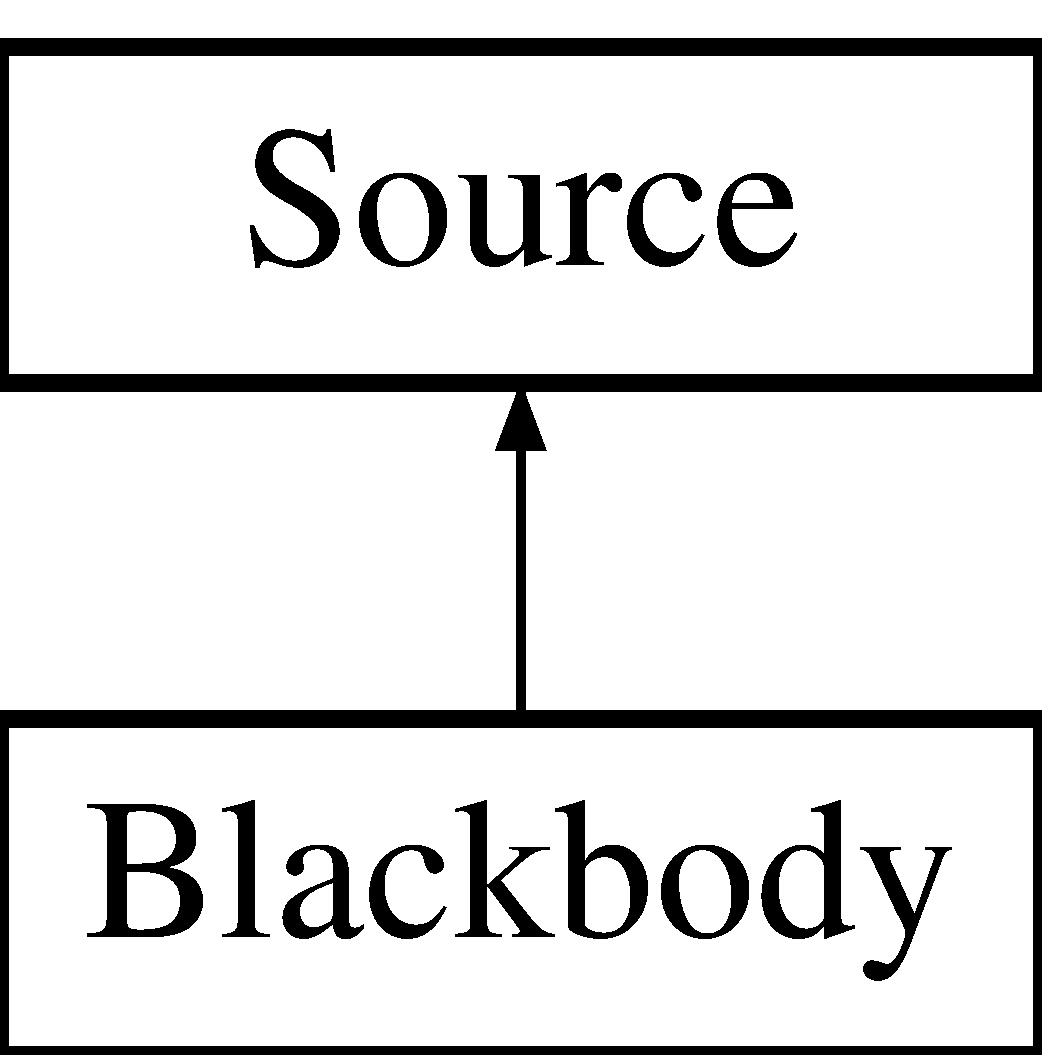
\includegraphics[height=2.000000cm]{class_blackbody}
\end{center}
\end{figure}
\subsection*{Public Member Functions}
\begin{DoxyCompactItemize}
\item 
\hyperlink{class_blackbody_a4461b2a29dd0ee94ec0d23c7a936c4ce}{Blackbody} (double \hyperlink{class_blackbody_ab565e14b93a8459ebbd4e2c5583932f0}{T})
\item 
double \hyperlink{class_blackbody_a2e667cd4c4362550a77eb9081258ffb3}{get\+\_\+spectral\+\_\+density} (double wavelength)
\end{DoxyCompactItemize}
\subsection*{Static Public Member Functions}
\begin{DoxyCompactItemize}
\item 
static double \hyperlink{class_blackbody_a7c2d99ba62b8d499de07edaabdc3b7f9}{planck} (const double \&\hyperlink{class_blackbody_ab565e14b93a8459ebbd4e2c5583932f0}{T}, const double \&wavelength)
\end{DoxyCompactItemize}
\subsection*{Private Attributes}
\begin{DoxyCompactItemize}
\item 
double \hyperlink{class_blackbody_ab565e14b93a8459ebbd4e2c5583932f0}{T}
\begin{DoxyCompactList}\small\item\em Temperature \mbox{[}K\mbox{]}. \end{DoxyCompactList}\end{DoxyCompactItemize}


\subsection{Detailed Description}
Implements a {\itshape blackbody spectrum.} 

This class implements the spectrum of a blackbody of a certain Temperature. \begin{DoxySeeAlso}{See also}
\{\hyperlink{class_blackbody_a2e667cd4c4362550a77eb9081258ffb3}{Blackbody\+::get\+\_\+spectral\+\_\+density()}\}
\end{DoxySeeAlso}
\[ \fbox{ \begin{tikzpicture} \begin{axis}[domain=300E-9:4000E-9, samples=100] \addplot[color=red]{2.0 *6.62606896E-34* 2.9979E8 * 2.9979E8 / (x^5)*1./(exp(6.62606896E-34*2.997E8/(x*1.3806504E-23*3500))-1)}; \end{axis} \end{tikzpicture} } \] 

\subsection{Constructor \& Destructor Documentation}
\index{Blackbody@{Blackbody}!Blackbody@{Blackbody}}
\index{Blackbody@{Blackbody}!Blackbody@{Blackbody}}
\subsubsection[{\texorpdfstring{Blackbody(double T)}{Blackbody(double T)}}]{\setlength{\rightskip}{0pt plus 5cm}Blackbody\+::\+Blackbody (
\begin{DoxyParamCaption}
\item[{double}]{T}
\end{DoxyParamCaption}
)}\hypertarget{class_blackbody_a4461b2a29dd0ee94ec0d23c7a936c4ce}{}\label{class_blackbody_a4461b2a29dd0ee94ec0d23c7a936c4ce}
Constructor 
\begin{DoxyParams}{Parameters}
{\em T} & Temperature \mbox{[}K\mbox{]} \\
\hline
\end{DoxyParams}


\subsection{Member Function Documentation}
\index{Blackbody@{Blackbody}!get\+\_\+spectral\+\_\+density@{get\+\_\+spectral\+\_\+density}}
\index{get\+\_\+spectral\+\_\+density@{get\+\_\+spectral\+\_\+density}!Blackbody@{Blackbody}}
\subsubsection[{\texorpdfstring{get\+\_\+spectral\+\_\+density(double wavelength)}{get_spectral_density(double wavelength)}}]{\setlength{\rightskip}{0pt plus 5cm}double Blackbody\+::get\+\_\+spectral\+\_\+density (
\begin{DoxyParamCaption}
\item[{double}]{wavelength}
\end{DoxyParamCaption}
)\hspace{0.3cm}{\ttfamily [virtual]}}\hypertarget{class_blackbody_a2e667cd4c4362550a77eb9081258ffb3}{}\label{class_blackbody_a2e667cd4c4362550a77eb9081258ffb3}
spectral density of a blackbody \[ s(\lambda) = \frac{2hc^2}{\lambda^5}\frac{1}{\exp{\frac{hc}{\lambda k_B T}}-1} \] 
\begin{DoxyParams}{Parameters}
{\em wavelength} & wavelength \mbox{[}micron\mbox{]} \\
\hline
\end{DoxyParams}
\begin{DoxyReturn}{Returns}
spectral density of a blackbody at given wavelength 
\end{DoxyReturn}


Reimplemented from \hyperlink{class_source_a546ae8ec1ae47e888c74f146278e19af}{Source}.

\index{Blackbody@{Blackbody}!planck@{planck}}
\index{planck@{planck}!Blackbody@{Blackbody}}
\subsubsection[{\texorpdfstring{planck(const double \&\+T, const double \&wavelength)}{planck(const double &T, const double &wavelength)}}]{\setlength{\rightskip}{0pt plus 5cm}double Blackbody\+::planck (
\begin{DoxyParamCaption}
\item[{const double \&}]{T, }
\item[{const double \&}]{wavelength}
\end{DoxyParamCaption}
)\hspace{0.3cm}{\ttfamily [static]}}\hypertarget{class_blackbody_a7c2d99ba62b8d499de07edaabdc3b7f9}{}\label{class_blackbody_a7c2d99ba62b8d499de07edaabdc3b7f9}
Planck function for spectral density of a blackbody with Temperature T 
\begin{DoxyParams}{Parameters}
{\em T} & Temperature \mbox{[}K\mbox{]} \\
\hline
{\em wavelength} & wavelength \mbox{[}m\mbox{]} \\
\hline
\end{DoxyParams}
\begin{DoxyReturn}{Returns}
spectral density 
\end{DoxyReturn}


\subsection{Member Data Documentation}
\index{Blackbody@{Blackbody}!T@{T}}
\index{T@{T}!Blackbody@{Blackbody}}
\subsubsection[{\texorpdfstring{T}{T}}]{\setlength{\rightskip}{0pt plus 5cm}double Blackbody\+::T\hspace{0.3cm}{\ttfamily [private]}}\hypertarget{class_blackbody_ab565e14b93a8459ebbd4e2c5583932f0}{}\label{class_blackbody_ab565e14b93a8459ebbd4e2c5583932f0}


Temperature \mbox{[}K\mbox{]}. 



The documentation for this class was generated from the following files\+:\begin{DoxyCompactItemize}
\item 
/home/stuermer/\+Repos/cpp/\+Echelle\+Simulator/include/\hyperlink{source_8h}{source.\+h}\item 
/home/stuermer/\+Repos/cpp/\+Echelle\+Simulator/src/\hyperlink{source_8cpp}{source.\+cpp}\end{DoxyCompactItemize}

\hypertarget{class_c_c_d}{}\section{C\+CD Class Reference}
\label{class_c_c_d}\index{C\+CD@{C\+CD}}


class representing a \hyperlink{class_c_c_d}{C\+CD} detector  




{\ttfamily \#include $<$C\+C\+D.\+h$>$}

\subsection*{Public Member Functions}
\begin{DoxyCompactItemize}
\item 
\hyperlink{class_c_c_d_a61f17e0715aada9a29906ff5486d448b}{C\+CD} (int \hyperlink{class_c_c_d_abe89ab0452f494147601a5c323e52588}{Nx}, int \hyperlink{class_c_c_d_a31f3c760f9ead50dbd3c7272314ddc9e}{Ny}, int \hyperlink{class_c_c_d_a147d14d779dc54c05b3fc65a4e97c698}{oversampling}, int data\+\_\+type)
\item 
\hyperlink{class_c_c_d_abec74b1675c8313078686c62596cc104}{$\sim$\+C\+CD} ()
\item 
void \hyperlink{class_c_c_d_a2c03b076762520d22424f765f97691f7}{save\+\_\+to\+\_\+file} (std\+::string filename, bool downsample=true, bool bleed=true, bool overwrite=false)
\item 
cv\+::\+Mat \hyperlink{class_c_c_d_ae3a55b1799c2e4f25cef3160f6d65c68}{get\+\_\+image} (bool downsample=true, bool bleed=true)
\item 
\hyperlink{class_c_c_d}{C\+CD} \hyperlink{class_c_c_d_addede6d5e44ddb13370396c77fbf7178}{operator+} (const \hyperlink{class_c_c_d}{C\+CD} \&ccd)
\end{DoxyCompactItemize}
\subsection*{Static Public Member Functions}
\begin{DoxyCompactItemize}
\item 
static void \hyperlink{class_c_c_d_ab04045e3277a84af6e1cefc24ede448c}{do\+\_\+bleed} (cv\+::\+Mat \&input, double limit)
\end{DoxyCompactItemize}
\subsection*{Public Attributes}
\begin{DoxyCompactItemize}
\item 
cv\+::\+Mat \hyperlink{class_c_c_d_abb1dc40d976f69d6a8ce01c407810e6b}{data}
\item 
bool \hyperlink{class_c_c_d_abeed44146ecffcd143263700413a41bd}{use\+\_\+gpu} = false
\end{DoxyCompactItemize}
\subsection*{Private Attributes}
\begin{DoxyCompactItemize}
\item 
int \hyperlink{class_c_c_d_abe89ab0452f494147601a5c323e52588}{Nx}
\item 
int \hyperlink{class_c_c_d_a31f3c760f9ead50dbd3c7272314ddc9e}{Ny}
\item 
int \hyperlink{class_c_c_d_a147d14d779dc54c05b3fc65a4e97c698}{oversampling}
\end{DoxyCompactItemize}


\subsection{Detailed Description}
class representing a \hyperlink{class_c_c_d}{C\+CD} detector 

\subsection{Constructor \& Destructor Documentation}
\index{C\+CD@{C\+CD}!C\+CD@{C\+CD}}
\index{C\+CD@{C\+CD}!C\+CD@{C\+CD}}
\subsubsection[{\texorpdfstring{C\+C\+D(int Nx, int Ny, int oversampling, int data\+\_\+type)}{CCD(int Nx, int Ny, int oversampling, int data_type)}}]{\setlength{\rightskip}{0pt plus 5cm}C\+C\+D\+::\+C\+CD (
\begin{DoxyParamCaption}
\item[{int}]{Nx, }
\item[{int}]{Ny, }
\item[{int}]{oversampling, }
\item[{int}]{data\+\_\+type}
\end{DoxyParamCaption}
)}\hypertarget{class_c_c_d_a61f17e0715aada9a29906ff5486d448b}{}\label{class_c_c_d_a61f17e0715aada9a29906ff5486d448b}
Constructor 
\begin{DoxyParams}{Parameters}
{\em Nx} & number of pixels in X direction \\
\hline
{\em Ny} & number of pixels in Y direction \\
\hline
{\em oversampling} & specifies the oversampling factor that will be used to downsample the image to its physical size \\
\hline
{\em data\+\_\+type} & data type, should be same as slit.\+image. Possible values see opencv datatypes (e.\+g. C\+V\+\_\+32F, C\+V\+\_\+64F,...) \\
\hline
\end{DoxyParams}
\begin{DoxyReturn}{Returns}
\hyperlink{class_c_c_d}{C\+CD} 
\end{DoxyReturn}
\index{C\+CD@{C\+CD}!````~C\+CD@{$\sim$\+C\+CD}}
\index{````~C\+CD@{$\sim$\+C\+CD}!C\+CD@{C\+CD}}
\subsubsection[{\texorpdfstring{$\sim$\+C\+C\+D()}{~CCD()}}]{\setlength{\rightskip}{0pt plus 5cm}C\+C\+D\+::$\sim$\+C\+CD (
\begin{DoxyParamCaption}
{}
\end{DoxyParamCaption}
)}\hypertarget{class_c_c_d_abec74b1675c8313078686c62596cc104}{}\label{class_c_c_d_abec74b1675c8313078686c62596cc104}


\subsection{Member Function Documentation}
\index{C\+CD@{C\+CD}!do\+\_\+bleed@{do\+\_\+bleed}}
\index{do\+\_\+bleed@{do\+\_\+bleed}!C\+CD@{C\+CD}}
\subsubsection[{\texorpdfstring{do\+\_\+bleed(cv\+::\+Mat \&input, double limit)}{do_bleed(cv::Mat &input, double limit)}}]{\setlength{\rightskip}{0pt plus 5cm}void C\+C\+D\+::do\+\_\+bleed (
\begin{DoxyParamCaption}
\item[{cv\+::\+Mat \&}]{input, }
\item[{double}]{limit}
\end{DoxyParamCaption}
)\hspace{0.3cm}{\ttfamily [static]}}\hypertarget{class_c_c_d_ab04045e3277a84af6e1cefc24ede448c}{}\label{class_c_c_d_ab04045e3277a84af6e1cefc24ede448c}
\index{C\+CD@{C\+CD}!get\+\_\+image@{get\+\_\+image}}
\index{get\+\_\+image@{get\+\_\+image}!C\+CD@{C\+CD}}
\subsubsection[{\texorpdfstring{get\+\_\+image(bool downsample=true, bool bleed=true)}{get_image(bool downsample=true, bool bleed=true)}}]{\setlength{\rightskip}{0pt plus 5cm}cv\+::\+Mat C\+C\+D\+::get\+\_\+image (
\begin{DoxyParamCaption}
\item[{bool}]{downsample = {\ttfamily true}, }
\item[{bool}]{bleed = {\ttfamily true}}
\end{DoxyParamCaption}
)}\hypertarget{class_c_c_d_ae3a55b1799c2e4f25cef3160f6d65c68}{}\label{class_c_c_d_ae3a55b1799c2e4f25cef3160f6d65c68}
\index{C\+CD@{C\+CD}!operator+@{operator+}}
\index{operator+@{operator+}!C\+CD@{C\+CD}}
\subsubsection[{\texorpdfstring{operator+(const C\+C\+D \&ccd)}{operator+(const CCD &ccd)}}]{\setlength{\rightskip}{0pt plus 5cm}{\bf C\+CD} C\+C\+D\+::operator+ (
\begin{DoxyParamCaption}
\item[{const {\bf C\+CD} \&}]{ccd}
\end{DoxyParamCaption}
)\hspace{0.3cm}{\ttfamily [inline]}}\hypertarget{class_c_c_d_addede6d5e44ddb13370396c77fbf7178}{}\label{class_c_c_d_addede6d5e44ddb13370396c77fbf7178}
\index{C\+CD@{C\+CD}!save\+\_\+to\+\_\+file@{save\+\_\+to\+\_\+file}}
\index{save\+\_\+to\+\_\+file@{save\+\_\+to\+\_\+file}!C\+CD@{C\+CD}}
\subsubsection[{\texorpdfstring{save\+\_\+to\+\_\+file(std\+::string filename, bool downsample=true, bool bleed=true, bool overwrite=false)}{save_to_file(std::string filename, bool downsample=true, bool bleed=true, bool overwrite=false)}}]{\setlength{\rightskip}{0pt plus 5cm}void C\+C\+D\+::save\+\_\+to\+\_\+file (
\begin{DoxyParamCaption}
\item[{std\+::string}]{filename, }
\item[{bool}]{downsample = {\ttfamily true}, }
\item[{bool}]{bleed = {\ttfamily true}, }
\item[{bool}]{overwrite = {\ttfamily false}}
\end{DoxyParamCaption}
)}\hypertarget{class_c_c_d_a2c03b076762520d22424f765f97691f7}{}\label{class_c_c_d_a2c03b076762520d22424f765f97691f7}


\subsection{Member Data Documentation}
\index{C\+CD@{C\+CD}!data@{data}}
\index{data@{data}!C\+CD@{C\+CD}}
\subsubsection[{\texorpdfstring{data}{data}}]{\setlength{\rightskip}{0pt plus 5cm}cv\+::\+Mat C\+C\+D\+::data}\hypertarget{class_c_c_d_abb1dc40d976f69d6a8ce01c407810e6b}{}\label{class_c_c_d_abb1dc40d976f69d6a8ce01c407810e6b}
\index{C\+CD@{C\+CD}!Nx@{Nx}}
\index{Nx@{Nx}!C\+CD@{C\+CD}}
\subsubsection[{\texorpdfstring{Nx}{Nx}}]{\setlength{\rightskip}{0pt plus 5cm}int C\+C\+D\+::\+Nx\hspace{0.3cm}{\ttfamily [private]}}\hypertarget{class_c_c_d_abe89ab0452f494147601a5c323e52588}{}\label{class_c_c_d_abe89ab0452f494147601a5c323e52588}
\index{C\+CD@{C\+CD}!Ny@{Ny}}
\index{Ny@{Ny}!C\+CD@{C\+CD}}
\subsubsection[{\texorpdfstring{Ny}{Ny}}]{\setlength{\rightskip}{0pt plus 5cm}int C\+C\+D\+::\+Ny\hspace{0.3cm}{\ttfamily [private]}}\hypertarget{class_c_c_d_a31f3c760f9ead50dbd3c7272314ddc9e}{}\label{class_c_c_d_a31f3c760f9ead50dbd3c7272314ddc9e}
\index{C\+CD@{C\+CD}!oversampling@{oversampling}}
\index{oversampling@{oversampling}!C\+CD@{C\+CD}}
\subsubsection[{\texorpdfstring{oversampling}{oversampling}}]{\setlength{\rightskip}{0pt plus 5cm}int C\+C\+D\+::oversampling\hspace{0.3cm}{\ttfamily [private]}}\hypertarget{class_c_c_d_a147d14d779dc54c05b3fc65a4e97c698}{}\label{class_c_c_d_a147d14d779dc54c05b3fc65a4e97c698}
\index{C\+CD@{C\+CD}!use\+\_\+gpu@{use\+\_\+gpu}}
\index{use\+\_\+gpu@{use\+\_\+gpu}!C\+CD@{C\+CD}}
\subsubsection[{\texorpdfstring{use\+\_\+gpu}{use_gpu}}]{\setlength{\rightskip}{0pt plus 5cm}bool C\+C\+D\+::use\+\_\+gpu = false}\hypertarget{class_c_c_d_abeed44146ecffcd143263700413a41bd}{}\label{class_c_c_d_abeed44146ecffcd143263700413a41bd}


The documentation for this class was generated from the following files\+:\begin{DoxyCompactItemize}
\item 
/home/stuermer/\+Repos/cpp/\+Echelle\+Simulator/include/\hyperlink{_c_c_d_8h}{C\+C\+D.\+h}\item 
/home/stuermer/\+Repos/cpp/\+Echelle\+Simulator/src/\hyperlink{_c_c_d_8cpp}{C\+C\+D.\+cpp}\end{DoxyCompactItemize}

\hypertarget{class_constant}{}\section{Constant Class Reference}
\label{class_constant}\index{Constant@{Constant}}


Implements constant spectral density.  




{\ttfamily \#include $<$source.\+h$>$}

Inheritance diagram for Constant\+:\begin{figure}[H]
\begin{center}
\leavevmode
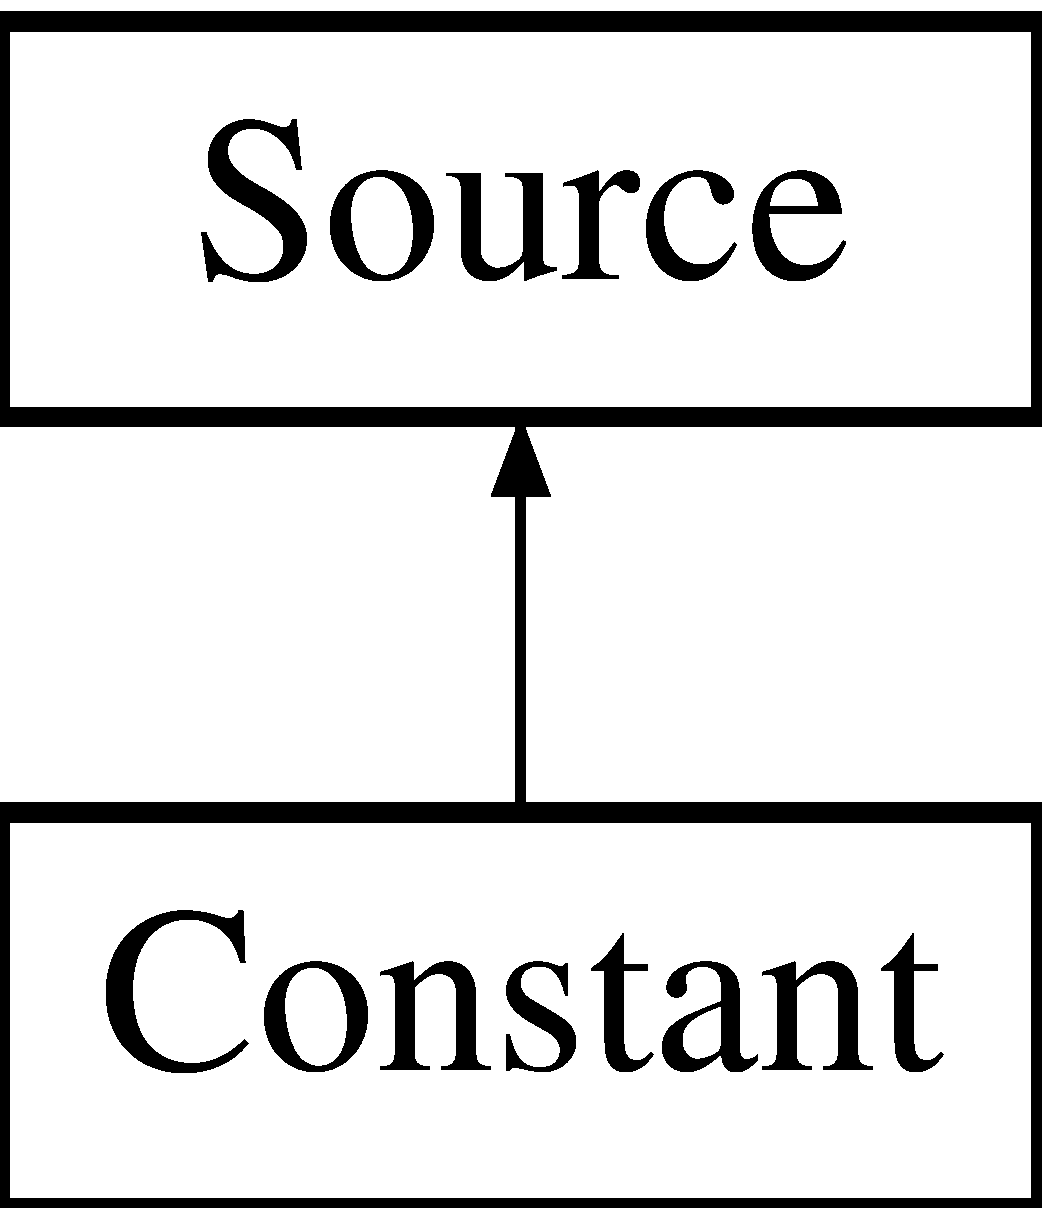
\includegraphics[height=2.000000cm]{class_constant}
\end{center}
\end{figure}
\subsection*{Public Member Functions}
\begin{DoxyCompactItemize}
\item 
\hyperlink{class_constant_a6d2f7d070d22aed4a3371c181da67716}{Constant} ()
\item 
\hyperlink{class_constant_aeecd18786af94c7e91a0497438caacf9}{Constant} (double \hyperlink{class_constant_ac48c9f0bb497a075190f43f2981ac5e7}{value})
\item 
double \hyperlink{class_constant_ae0526443e519154bcd338ee930bcad04}{get\+\_\+spectral\+\_\+density} (double wavelength)
\end{DoxyCompactItemize}
\subsection*{Private Attributes}
\begin{DoxyCompactItemize}
\item 
double \hyperlink{class_constant_ac48c9f0bb497a075190f43f2981ac5e7}{value}
\end{DoxyCompactItemize}


\subsection{Detailed Description}
Implements constant spectral density. 

This class implements a constant spectral density. \[ s(\lambda) = const. \] 

\subsection{Constructor \& Destructor Documentation}
\index{Constant@{Constant}!Constant@{Constant}}
\index{Constant@{Constant}!Constant@{Constant}}
\subsubsection[{\texorpdfstring{Constant()}{Constant()}}]{\setlength{\rightskip}{0pt plus 5cm}Constant\+::\+Constant (
\begin{DoxyParamCaption}
{}
\end{DoxyParamCaption}
)}\hypertarget{class_constant_a6d2f7d070d22aed4a3371c181da67716}{}\label{class_constant_a6d2f7d070d22aed4a3371c181da67716}
\index{Constant@{Constant}!Constant@{Constant}}
\index{Constant@{Constant}!Constant@{Constant}}
\subsubsection[{\texorpdfstring{Constant(double value)}{Constant(double value)}}]{\setlength{\rightskip}{0pt plus 5cm}Constant\+::\+Constant (
\begin{DoxyParamCaption}
\item[{double}]{value}
\end{DoxyParamCaption}
)}\hypertarget{class_constant_aeecd18786af94c7e91a0497438caacf9}{}\label{class_constant_aeecd18786af94c7e91a0497438caacf9}
Constructor 
\begin{DoxyParams}{Parameters}
{\em value} & constant spectral density value \\
\hline
\end{DoxyParams}


\subsection{Member Function Documentation}
\index{Constant@{Constant}!get\+\_\+spectral\+\_\+density@{get\+\_\+spectral\+\_\+density}}
\index{get\+\_\+spectral\+\_\+density@{get\+\_\+spectral\+\_\+density}!Constant@{Constant}}
\subsubsection[{\texorpdfstring{get\+\_\+spectral\+\_\+density(double wavelength)}{get_spectral_density(double wavelength)}}]{\setlength{\rightskip}{0pt plus 5cm}double Constant\+::get\+\_\+spectral\+\_\+density (
\begin{DoxyParamCaption}
\item[{double}]{wavelength}
\end{DoxyParamCaption}
)\hspace{0.3cm}{\ttfamily [virtual]}}\hypertarget{class_constant_ae0526443e519154bcd338ee930bcad04}{}\label{class_constant_ae0526443e519154bcd338ee930bcad04}
Returns constant spectral density.


\begin{DoxyParams}{Parameters}
{\em wavelength} & wavelength \\
\hline
\end{DoxyParams}
\begin{DoxyReturn}{Returns}
constant spectral density value 
\end{DoxyReturn}


Reimplemented from \hyperlink{class_source_a546ae8ec1ae47e888c74f146278e19af}{Source}.



\subsection{Member Data Documentation}
\index{Constant@{Constant}!value@{value}}
\index{value@{value}!Constant@{Constant}}
\subsubsection[{\texorpdfstring{value}{value}}]{\setlength{\rightskip}{0pt plus 5cm}double Constant\+::value\hspace{0.3cm}{\ttfamily [private]}}\hypertarget{class_constant_ac48c9f0bb497a075190f43f2981ac5e7}{}\label{class_constant_ac48c9f0bb497a075190f43f2981ac5e7}


The documentation for this class was generated from the following files\+:\begin{DoxyCompactItemize}
\item 
/home/stuermer/\+Repos/cpp/\+Echelle\+Simulator/include/\hyperlink{source_8h}{source.\+h}\item 
/home/stuermer/\+Repos/cpp/\+Echelle\+Simulator/src/\hyperlink{source_8cpp}{source.\+cpp}\end{DoxyCompactItemize}

\hypertarget{class_c_s_v_iterator}{}\section{C\+S\+V\+Iterator Class Reference}
\label{class_c_s_v_iterator}\index{C\+S\+V\+Iterator@{C\+S\+V\+Iterator}}


{\ttfamily \#include $<$csv\+\_\+reader.\+h$>$}

\subsection*{Public Types}
\begin{DoxyCompactItemize}
\item 
typedef std\+::input\+\_\+iterator\+\_\+tag \hyperlink{class_c_s_v_iterator_a1e8e34ec6798b67292c1b1b9bf18e8f6}{iterator\+\_\+category}
\item 
typedef \hyperlink{class_c_s_v_row}{C\+S\+V\+Row} \hyperlink{class_c_s_v_iterator_a86931db4489064aa95164fee9123d40e}{value\+\_\+type}
\item 
typedef std\+::size\+\_\+t \hyperlink{class_c_s_v_iterator_a2decbf132c26754c9a32402b7bc9848f}{difference\+\_\+type}
\item 
typedef \hyperlink{class_c_s_v_row}{C\+S\+V\+Row} $\ast$ \hyperlink{class_c_s_v_iterator_a23ee3d00badf18d56739868b4f0c0240}{pointer}
\item 
typedef \hyperlink{class_c_s_v_row}{C\+S\+V\+Row} \& \hyperlink{class_c_s_v_iterator_a4f99b48a9e06dec230dda0b073d07d9e}{reference}
\end{DoxyCompactItemize}
\subsection*{Public Member Functions}
\begin{DoxyCompactItemize}
\item 
\hyperlink{class_c_s_v_iterator_a5e1ec4423e05bf23c4209f3089d8e0b2}{C\+S\+V\+Iterator} (std\+::istream \&str)
\item 
\hyperlink{class_c_s_v_iterator_a8c3e1708c84d80dc8b51822547f2c2aa}{C\+S\+V\+Iterator} ()
\item 
\hyperlink{class_c_s_v_iterator}{C\+S\+V\+Iterator} \& \hyperlink{class_c_s_v_iterator_a5bac2b8aaf235c2ee1b0b2b9da9b3399}{operator++} ()
\item 
\hyperlink{class_c_s_v_iterator}{C\+S\+V\+Iterator} \hyperlink{class_c_s_v_iterator_ab3f320940c36f5524865b349e6d1b36b}{operator++} (int)
\item 
\hyperlink{class_c_s_v_row}{C\+S\+V\+Row} const \& \hyperlink{class_c_s_v_iterator_a0577e6c41cd7f595762f84736d751c38}{operator$\ast$} () const 
\item 
\hyperlink{class_c_s_v_row}{C\+S\+V\+Row} const $\ast$ \hyperlink{class_c_s_v_iterator_aea83ae54c091c545a462d4152e06bf5f}{operator-\/$>$} () const 
\item 
bool \hyperlink{class_c_s_v_iterator_a75dbe096c1a074b74dadd7ab2283f3e9}{operator==} (\hyperlink{class_c_s_v_iterator}{C\+S\+V\+Iterator} const \&rhs)
\item 
bool \hyperlink{class_c_s_v_iterator_a4ba4b13be1e878cfd1a9c9e6d69f9a62}{operator!=} (\hyperlink{class_c_s_v_iterator}{C\+S\+V\+Iterator} const \&rhs)
\end{DoxyCompactItemize}
\subsection*{Private Attributes}
\begin{DoxyCompactItemize}
\item 
std\+::istream $\ast$ \hyperlink{class_c_s_v_iterator_abb34432d545dcb80447b020fe8a47cad}{m\+\_\+str}
\item 
\hyperlink{class_c_s_v_row}{C\+S\+V\+Row} \hyperlink{class_c_s_v_iterator_a051522e4a6e5097f0348869455c2eddd}{m\+\_\+row}
\end{DoxyCompactItemize}


\subsection{Member Typedef Documentation}
\index{C\+S\+V\+Iterator@{C\+S\+V\+Iterator}!difference\+\_\+type@{difference\+\_\+type}}
\index{difference\+\_\+type@{difference\+\_\+type}!C\+S\+V\+Iterator@{C\+S\+V\+Iterator}}
\subsubsection[{\texorpdfstring{difference\+\_\+type}{difference_type}}]{\setlength{\rightskip}{0pt plus 5cm}typedef std\+::size\+\_\+t {\bf C\+S\+V\+Iterator\+::difference\+\_\+type}}\hypertarget{class_c_s_v_iterator_a2decbf132c26754c9a32402b7bc9848f}{}\label{class_c_s_v_iterator_a2decbf132c26754c9a32402b7bc9848f}
\index{C\+S\+V\+Iterator@{C\+S\+V\+Iterator}!iterator\+\_\+category@{iterator\+\_\+category}}
\index{iterator\+\_\+category@{iterator\+\_\+category}!C\+S\+V\+Iterator@{C\+S\+V\+Iterator}}
\subsubsection[{\texorpdfstring{iterator\+\_\+category}{iterator_category}}]{\setlength{\rightskip}{0pt plus 5cm}typedef std\+::input\+\_\+iterator\+\_\+tag {\bf C\+S\+V\+Iterator\+::iterator\+\_\+category}}\hypertarget{class_c_s_v_iterator_a1e8e34ec6798b67292c1b1b9bf18e8f6}{}\label{class_c_s_v_iterator_a1e8e34ec6798b67292c1b1b9bf18e8f6}
\index{C\+S\+V\+Iterator@{C\+S\+V\+Iterator}!pointer@{pointer}}
\index{pointer@{pointer}!C\+S\+V\+Iterator@{C\+S\+V\+Iterator}}
\subsubsection[{\texorpdfstring{pointer}{pointer}}]{\setlength{\rightskip}{0pt plus 5cm}typedef {\bf C\+S\+V\+Row}$\ast$ {\bf C\+S\+V\+Iterator\+::pointer}}\hypertarget{class_c_s_v_iterator_a23ee3d00badf18d56739868b4f0c0240}{}\label{class_c_s_v_iterator_a23ee3d00badf18d56739868b4f0c0240}
\index{C\+S\+V\+Iterator@{C\+S\+V\+Iterator}!reference@{reference}}
\index{reference@{reference}!C\+S\+V\+Iterator@{C\+S\+V\+Iterator}}
\subsubsection[{\texorpdfstring{reference}{reference}}]{\setlength{\rightskip}{0pt plus 5cm}typedef {\bf C\+S\+V\+Row}\& {\bf C\+S\+V\+Iterator\+::reference}}\hypertarget{class_c_s_v_iterator_a4f99b48a9e06dec230dda0b073d07d9e}{}\label{class_c_s_v_iterator_a4f99b48a9e06dec230dda0b073d07d9e}
\index{C\+S\+V\+Iterator@{C\+S\+V\+Iterator}!value\+\_\+type@{value\+\_\+type}}
\index{value\+\_\+type@{value\+\_\+type}!C\+S\+V\+Iterator@{C\+S\+V\+Iterator}}
\subsubsection[{\texorpdfstring{value\+\_\+type}{value_type}}]{\setlength{\rightskip}{0pt plus 5cm}typedef {\bf C\+S\+V\+Row} {\bf C\+S\+V\+Iterator\+::value\+\_\+type}}\hypertarget{class_c_s_v_iterator_a86931db4489064aa95164fee9123d40e}{}\label{class_c_s_v_iterator_a86931db4489064aa95164fee9123d40e}


\subsection{Constructor \& Destructor Documentation}
\index{C\+S\+V\+Iterator@{C\+S\+V\+Iterator}!C\+S\+V\+Iterator@{C\+S\+V\+Iterator}}
\index{C\+S\+V\+Iterator@{C\+S\+V\+Iterator}!C\+S\+V\+Iterator@{C\+S\+V\+Iterator}}
\subsubsection[{\texorpdfstring{C\+S\+V\+Iterator(std\+::istream \&str)}{CSVIterator(std::istream &str)}}]{\setlength{\rightskip}{0pt plus 5cm}C\+S\+V\+Iterator\+::\+C\+S\+V\+Iterator (
\begin{DoxyParamCaption}
\item[{std\+::istream \&}]{str}
\end{DoxyParamCaption}
)\hspace{0.3cm}{\ttfamily [inline]}}\hypertarget{class_c_s_v_iterator_a5e1ec4423e05bf23c4209f3089d8e0b2}{}\label{class_c_s_v_iterator_a5e1ec4423e05bf23c4209f3089d8e0b2}
\index{C\+S\+V\+Iterator@{C\+S\+V\+Iterator}!C\+S\+V\+Iterator@{C\+S\+V\+Iterator}}
\index{C\+S\+V\+Iterator@{C\+S\+V\+Iterator}!C\+S\+V\+Iterator@{C\+S\+V\+Iterator}}
\subsubsection[{\texorpdfstring{C\+S\+V\+Iterator()}{CSVIterator()}}]{\setlength{\rightskip}{0pt plus 5cm}C\+S\+V\+Iterator\+::\+C\+S\+V\+Iterator (
\begin{DoxyParamCaption}
{}
\end{DoxyParamCaption}
)\hspace{0.3cm}{\ttfamily [inline]}}\hypertarget{class_c_s_v_iterator_a8c3e1708c84d80dc8b51822547f2c2aa}{}\label{class_c_s_v_iterator_a8c3e1708c84d80dc8b51822547f2c2aa}


\subsection{Member Function Documentation}
\index{C\+S\+V\+Iterator@{C\+S\+V\+Iterator}!operator"!=@{operator"!=}}
\index{operator"!=@{operator"!=}!C\+S\+V\+Iterator@{C\+S\+V\+Iterator}}
\subsubsection[{\texorpdfstring{operator"!=(\+C\+S\+V\+Iterator const \&rhs)}{operator!=(CSVIterator const &rhs)}}]{\setlength{\rightskip}{0pt plus 5cm}bool C\+S\+V\+Iterator\+::operator!= (
\begin{DoxyParamCaption}
\item[{{\bf C\+S\+V\+Iterator} const \&}]{rhs}
\end{DoxyParamCaption}
)\hspace{0.3cm}{\ttfamily [inline]}}\hypertarget{class_c_s_v_iterator_a4ba4b13be1e878cfd1a9c9e6d69f9a62}{}\label{class_c_s_v_iterator_a4ba4b13be1e878cfd1a9c9e6d69f9a62}
\index{C\+S\+V\+Iterator@{C\+S\+V\+Iterator}!operator$\ast$@{operator$\ast$}}
\index{operator$\ast$@{operator$\ast$}!C\+S\+V\+Iterator@{C\+S\+V\+Iterator}}
\subsubsection[{\texorpdfstring{operator$\ast$() const }{operator*() const }}]{\setlength{\rightskip}{0pt plus 5cm}{\bf C\+S\+V\+Row} const\& C\+S\+V\+Iterator\+::operator$\ast$ (
\begin{DoxyParamCaption}
{}
\end{DoxyParamCaption}
) const\hspace{0.3cm}{\ttfamily [inline]}}\hypertarget{class_c_s_v_iterator_a0577e6c41cd7f595762f84736d751c38}{}\label{class_c_s_v_iterator_a0577e6c41cd7f595762f84736d751c38}
\index{C\+S\+V\+Iterator@{C\+S\+V\+Iterator}!operator++@{operator++}}
\index{operator++@{operator++}!C\+S\+V\+Iterator@{C\+S\+V\+Iterator}}
\subsubsection[{\texorpdfstring{operator++()}{operator++()}}]{\setlength{\rightskip}{0pt plus 5cm}{\bf C\+S\+V\+Iterator}\& C\+S\+V\+Iterator\+::operator++ (
\begin{DoxyParamCaption}
{}
\end{DoxyParamCaption}
)\hspace{0.3cm}{\ttfamily [inline]}}\hypertarget{class_c_s_v_iterator_a5bac2b8aaf235c2ee1b0b2b9da9b3399}{}\label{class_c_s_v_iterator_a5bac2b8aaf235c2ee1b0b2b9da9b3399}
\index{C\+S\+V\+Iterator@{C\+S\+V\+Iterator}!operator++@{operator++}}
\index{operator++@{operator++}!C\+S\+V\+Iterator@{C\+S\+V\+Iterator}}
\subsubsection[{\texorpdfstring{operator++(int)}{operator++(int)}}]{\setlength{\rightskip}{0pt plus 5cm}{\bf C\+S\+V\+Iterator} C\+S\+V\+Iterator\+::operator++ (
\begin{DoxyParamCaption}
\item[{int}]{}
\end{DoxyParamCaption}
)\hspace{0.3cm}{\ttfamily [inline]}}\hypertarget{class_c_s_v_iterator_ab3f320940c36f5524865b349e6d1b36b}{}\label{class_c_s_v_iterator_ab3f320940c36f5524865b349e6d1b36b}
\index{C\+S\+V\+Iterator@{C\+S\+V\+Iterator}!operator-\/$>$@{operator-\/$>$}}
\index{operator-\/$>$@{operator-\/$>$}!C\+S\+V\+Iterator@{C\+S\+V\+Iterator}}
\subsubsection[{\texorpdfstring{operator-\/$>$() const }{operator->() const }}]{\setlength{\rightskip}{0pt plus 5cm}{\bf C\+S\+V\+Row} const$\ast$ C\+S\+V\+Iterator\+::operator-\/$>$ (
\begin{DoxyParamCaption}
{}
\end{DoxyParamCaption}
) const\hspace{0.3cm}{\ttfamily [inline]}}\hypertarget{class_c_s_v_iterator_aea83ae54c091c545a462d4152e06bf5f}{}\label{class_c_s_v_iterator_aea83ae54c091c545a462d4152e06bf5f}
\index{C\+S\+V\+Iterator@{C\+S\+V\+Iterator}!operator==@{operator==}}
\index{operator==@{operator==}!C\+S\+V\+Iterator@{C\+S\+V\+Iterator}}
\subsubsection[{\texorpdfstring{operator==(\+C\+S\+V\+Iterator const \&rhs)}{operator==(CSVIterator const &rhs)}}]{\setlength{\rightskip}{0pt plus 5cm}bool C\+S\+V\+Iterator\+::operator== (
\begin{DoxyParamCaption}
\item[{{\bf C\+S\+V\+Iterator} const \&}]{rhs}
\end{DoxyParamCaption}
)\hspace{0.3cm}{\ttfamily [inline]}}\hypertarget{class_c_s_v_iterator_a75dbe096c1a074b74dadd7ab2283f3e9}{}\label{class_c_s_v_iterator_a75dbe096c1a074b74dadd7ab2283f3e9}


\subsection{Member Data Documentation}
\index{C\+S\+V\+Iterator@{C\+S\+V\+Iterator}!m\+\_\+row@{m\+\_\+row}}
\index{m\+\_\+row@{m\+\_\+row}!C\+S\+V\+Iterator@{C\+S\+V\+Iterator}}
\subsubsection[{\texorpdfstring{m\+\_\+row}{m_row}}]{\setlength{\rightskip}{0pt plus 5cm}{\bf C\+S\+V\+Row} C\+S\+V\+Iterator\+::m\+\_\+row\hspace{0.3cm}{\ttfamily [private]}}\hypertarget{class_c_s_v_iterator_a051522e4a6e5097f0348869455c2eddd}{}\label{class_c_s_v_iterator_a051522e4a6e5097f0348869455c2eddd}
\index{C\+S\+V\+Iterator@{C\+S\+V\+Iterator}!m\+\_\+str@{m\+\_\+str}}
\index{m\+\_\+str@{m\+\_\+str}!C\+S\+V\+Iterator@{C\+S\+V\+Iterator}}
\subsubsection[{\texorpdfstring{m\+\_\+str}{m_str}}]{\setlength{\rightskip}{0pt plus 5cm}std\+::istream$\ast$ C\+S\+V\+Iterator\+::m\+\_\+str\hspace{0.3cm}{\ttfamily [private]}}\hypertarget{class_c_s_v_iterator_abb34432d545dcb80447b020fe8a47cad}{}\label{class_c_s_v_iterator_abb34432d545dcb80447b020fe8a47cad}


The documentation for this class was generated from the following file\+:\begin{DoxyCompactItemize}
\item 
/home/stuermer/\+Repos/cpp/\+Echelle\+Simulator/include/\hyperlink{csv__reader_8h}{csv\+\_\+reader.\+h}\end{DoxyCompactItemize}

\hypertarget{class_c_s_v_row}{}\section{C\+S\+V\+Row Class Reference}
\label{class_c_s_v_row}\index{C\+S\+V\+Row@{C\+S\+V\+Row}}


{\ttfamily \#include $<$csv\+\_\+reader.\+h$>$}

\subsection*{Public Member Functions}
\begin{DoxyCompactItemize}
\item 
std\+::string const \& \hyperlink{class_c_s_v_row_ae44706c256795a7fbe21148305f076ba}{operator\mbox{[}$\,$\mbox{]}} (std\+::size\+\_\+t index) const 
\item 
std\+::size\+\_\+t \hyperlink{class_c_s_v_row_a3a1aae96182818cd3e32ce60f92d4d26}{size} () const 
\item 
void \hyperlink{class_c_s_v_row_a14b9ac6d9ffb01a7b05ea903cfd04eeb}{read\+Next\+Row} (std\+::istream \&str)
\end{DoxyCompactItemize}
\subsection*{Private Attributes}
\begin{DoxyCompactItemize}
\item 
std\+::vector$<$ std\+::string $>$ \hyperlink{class_c_s_v_row_a6ccfa2b79438ff191e0973c2e8f5fe1a}{m\+\_\+data}
\end{DoxyCompactItemize}


\subsection{Member Function Documentation}
\index{C\+S\+V\+Row@{C\+S\+V\+Row}!operator\mbox{[}$\,$\mbox{]}@{operator[]}}
\index{operator\mbox{[}$\,$\mbox{]}@{operator[]}!C\+S\+V\+Row@{C\+S\+V\+Row}}
\subsubsection[{\texorpdfstring{operator[](std\+::size\+\_\+t index) const }{operator[](std::size_t index) const }}]{\setlength{\rightskip}{0pt plus 5cm}std\+::string const\& C\+S\+V\+Row\+::operator\mbox{[}$\,$\mbox{]} (
\begin{DoxyParamCaption}
\item[{std\+::size\+\_\+t}]{index}
\end{DoxyParamCaption}
) const\hspace{0.3cm}{\ttfamily [inline]}}\hypertarget{class_c_s_v_row_ae44706c256795a7fbe21148305f076ba}{}\label{class_c_s_v_row_ae44706c256795a7fbe21148305f076ba}
\index{C\+S\+V\+Row@{C\+S\+V\+Row}!read\+Next\+Row@{read\+Next\+Row}}
\index{read\+Next\+Row@{read\+Next\+Row}!C\+S\+V\+Row@{C\+S\+V\+Row}}
\subsubsection[{\texorpdfstring{read\+Next\+Row(std\+::istream \&str)}{readNextRow(std::istream &str)}}]{\setlength{\rightskip}{0pt plus 5cm}void C\+S\+V\+Row\+::read\+Next\+Row (
\begin{DoxyParamCaption}
\item[{std\+::istream \&}]{str}
\end{DoxyParamCaption}
)\hspace{0.3cm}{\ttfamily [inline]}}\hypertarget{class_c_s_v_row_a14b9ac6d9ffb01a7b05ea903cfd04eeb}{}\label{class_c_s_v_row_a14b9ac6d9ffb01a7b05ea903cfd04eeb}
\index{C\+S\+V\+Row@{C\+S\+V\+Row}!size@{size}}
\index{size@{size}!C\+S\+V\+Row@{C\+S\+V\+Row}}
\subsubsection[{\texorpdfstring{size() const }{size() const }}]{\setlength{\rightskip}{0pt plus 5cm}std\+::size\+\_\+t C\+S\+V\+Row\+::size (
\begin{DoxyParamCaption}
{}
\end{DoxyParamCaption}
) const\hspace{0.3cm}{\ttfamily [inline]}}\hypertarget{class_c_s_v_row_a3a1aae96182818cd3e32ce60f92d4d26}{}\label{class_c_s_v_row_a3a1aae96182818cd3e32ce60f92d4d26}


\subsection{Member Data Documentation}
\index{C\+S\+V\+Row@{C\+S\+V\+Row}!m\+\_\+data@{m\+\_\+data}}
\index{m\+\_\+data@{m\+\_\+data}!C\+S\+V\+Row@{C\+S\+V\+Row}}
\subsubsection[{\texorpdfstring{m\+\_\+data}{m_data}}]{\setlength{\rightskip}{0pt plus 5cm}std\+::vector$<$std\+::string$>$ C\+S\+V\+Row\+::m\+\_\+data\hspace{0.3cm}{\ttfamily [private]}}\hypertarget{class_c_s_v_row_a6ccfa2b79438ff191e0973c2e8f5fe1a}{}\label{class_c_s_v_row_a6ccfa2b79438ff191e0973c2e8f5fe1a}


The documentation for this class was generated from the following file\+:\begin{DoxyCompactItemize}
\item 
/home/stuermer/\+Repos/cpp/\+Echelle\+Simulator/include/\hyperlink{csv__reader_8h}{csv\+\_\+reader.\+h}\end{DoxyCompactItemize}

\hypertarget{class_efficiency}{}\section{Efficiency Class Reference}
\label{class_efficiency}\index{Efficiency@{Efficiency}}


{\ttfamily \#include $<$efficiency.\+h$>$}

Inheritance diagram for Efficiency\+:\begin{figure}[H]
\begin{center}
\leavevmode
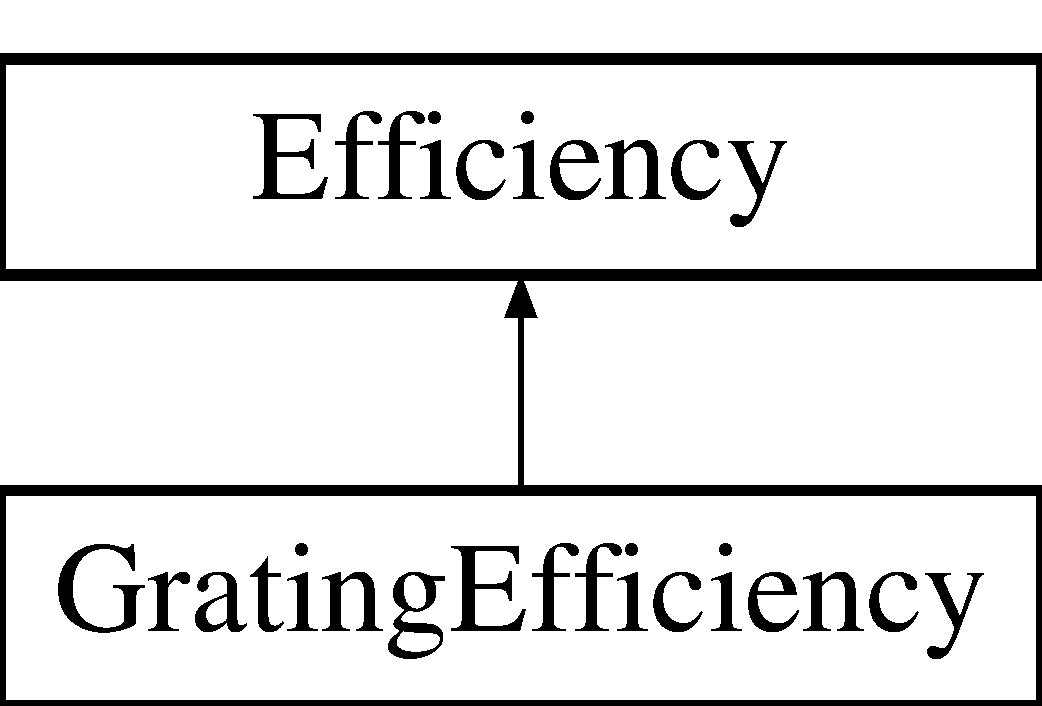
\includegraphics[height=2.000000cm]{class_efficiency}
\end{center}
\end{figure}
\subsection*{Public Member Functions}
\begin{DoxyCompactItemize}
\item 
\hyperlink{class_efficiency_ac21845145d2c817da1109d717a94c1e4}{Efficiency} ()
\item 
virtual \hyperlink{class_efficiency_a13ec7970ca3da052d642a0a79355d137}{$\sim$\+Efficiency} ()
\item 
virtual std\+::vector$<$ double $>$ \hyperlink{class_efficiency_aebed210f3588bc1cc43b75e2f2ed701e}{get\+\_\+efficieny} (int order, std\+::vector$<$ double $>$ wavelength)
\end{DoxyCompactItemize}


\subsection{Constructor \& Destructor Documentation}
\index{Efficiency@{Efficiency}!Efficiency@{Efficiency}}
\index{Efficiency@{Efficiency}!Efficiency@{Efficiency}}
\subsubsection[{\texorpdfstring{Efficiency()}{Efficiency()}}]{\setlength{\rightskip}{0pt plus 5cm}Efficiency\+::\+Efficiency (
\begin{DoxyParamCaption}
{}
\end{DoxyParamCaption}
)}\hypertarget{class_efficiency_ac21845145d2c817da1109d717a94c1e4}{}\label{class_efficiency_ac21845145d2c817da1109d717a94c1e4}
\index{Efficiency@{Efficiency}!````~Efficiency@{$\sim$\+Efficiency}}
\index{````~Efficiency@{$\sim$\+Efficiency}!Efficiency@{Efficiency}}
\subsubsection[{\texorpdfstring{$\sim$\+Efficiency()}{~Efficiency()}}]{\setlength{\rightskip}{0pt plus 5cm}Efficiency\+::$\sim$\+Efficiency (
\begin{DoxyParamCaption}
{}
\end{DoxyParamCaption}
)\hspace{0.3cm}{\ttfamily [virtual]}}\hypertarget{class_efficiency_a13ec7970ca3da052d642a0a79355d137}{}\label{class_efficiency_a13ec7970ca3da052d642a0a79355d137}


\subsection{Member Function Documentation}
\index{Efficiency@{Efficiency}!get\+\_\+efficieny@{get\+\_\+efficieny}}
\index{get\+\_\+efficieny@{get\+\_\+efficieny}!Efficiency@{Efficiency}}
\subsubsection[{\texorpdfstring{get\+\_\+efficieny(int order, std\+::vector$<$ double $>$ wavelength)}{get_efficieny(int order, std::vector< double > wavelength)}}]{\setlength{\rightskip}{0pt plus 5cm}std\+::vector$<$ double $>$ Efficiency\+::get\+\_\+efficieny (
\begin{DoxyParamCaption}
\item[{int}]{order, }
\item[{std\+::vector$<$ double $>$}]{wavelength}
\end{DoxyParamCaption}
)\hspace{0.3cm}{\ttfamily [virtual]}}\hypertarget{class_efficiency_aebed210f3588bc1cc43b75e2f2ed701e}{}\label{class_efficiency_aebed210f3588bc1cc43b75e2f2ed701e}


Reimplemented in \hyperlink{class_grating_efficiency_a0d0126c4618dbf976385d0126415195f}{Grating\+Efficiency}.



The documentation for this class was generated from the following files\+:\begin{DoxyCompactItemize}
\item 
/home/stuermer/\+Repos/cpp/\+Echelle\+Simulator/include/\hyperlink{efficiency_8h}{efficiency.\+h}\item 
/home/stuermer/\+Repos/cpp/\+Echelle\+Simulator/src/\hyperlink{efficiency_8cpp}{efficiency.\+cpp}\end{DoxyCompactItemize}

\hypertarget{class_grating_efficiency}{}\section{Grating\+Efficiency Class Reference}
\label{class_grating_efficiency}\index{Grating\+Efficiency@{Grating\+Efficiency}}


{\ttfamily \#include $<$efficiency.\+h$>$}

Inheritance diagram for Grating\+Efficiency\+:\begin{figure}[H]
\begin{center}
\leavevmode
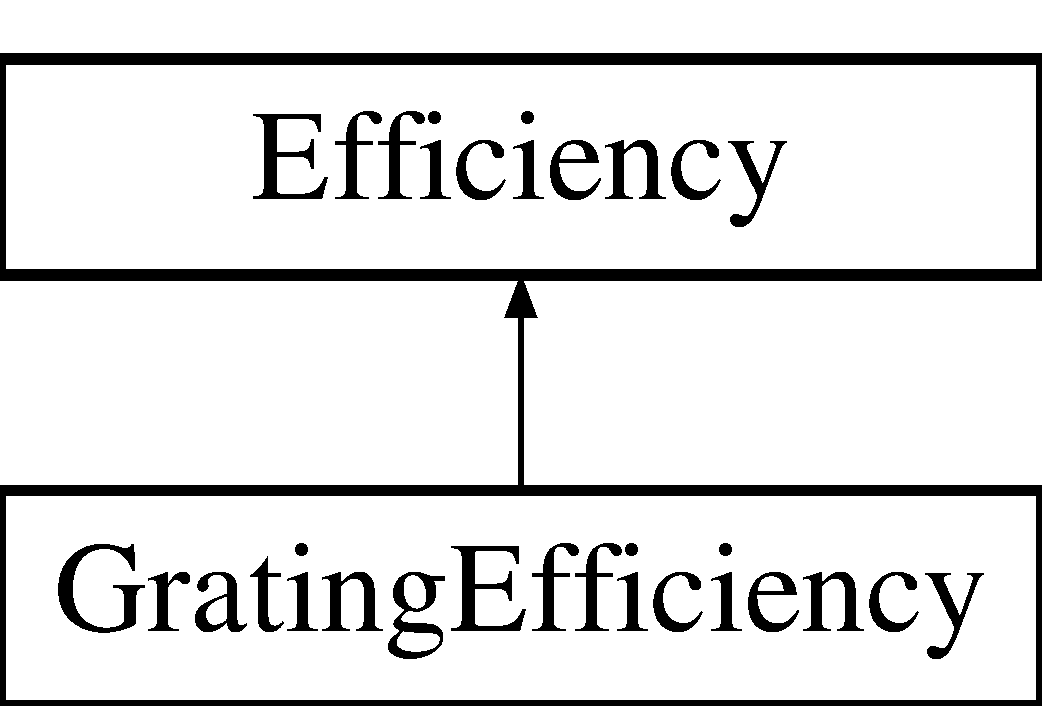
\includegraphics[height=2.000000cm]{class_grating_efficiency}
\end{center}
\end{figure}
\subsection*{Public Member Functions}
\begin{DoxyCompactItemize}
\item 
\hyperlink{class_grating_efficiency_a2c12fab8a296d57531239d9f653f57d7}{Grating\+Efficiency} (double \hyperlink{class_grating_efficiency_af452d057f148d401e9f2072e3752e0a4}{scalingfactor}, double \hyperlink{class_grating_efficiency_abb5fb732555147e8f977487d3a234c51}{alpha}, double \hyperlink{class_grating_efficiency_a541aa917f023bbb38025c271e3060d31}{blaze}, double \hyperlink{class_grating_efficiency_a3bbe348499e4b3d6792a2f8ecaca1f94}{gpmm})
\item 
std\+::vector$<$ double $>$ \hyperlink{class_grating_efficiency_a0d0126c4618dbf976385d0126415195f}{get\+\_\+efficieny} (int order, std\+::vector$<$ double $>$ wavelength)
\end{DoxyCompactItemize}
\subsection*{Private Member Functions}
\begin{DoxyCompactItemize}
\item 
double \hyperlink{class_grating_efficiency_a446eeb236e57ede246e96ebd863fa645}{calc\+\_\+eff} (double \hyperlink{class_grating_efficiency_af452d057f148d401e9f2072e3752e0a4}{scalingfactor}, int order, double \hyperlink{class_grating_efficiency_abb5fb732555147e8f977487d3a234c51}{alpha}, double \hyperlink{class_grating_efficiency_a541aa917f023bbb38025c271e3060d31}{blaze}, double wl, double n)
\end{DoxyCompactItemize}
\subsection*{Private Attributes}
\begin{DoxyCompactItemize}
\item 
double \hyperlink{class_grating_efficiency_af452d057f148d401e9f2072e3752e0a4}{scalingfactor} =0.\+8
\item 
double \hyperlink{class_grating_efficiency_abb5fb732555147e8f977487d3a234c51}{alpha} =76.
\item 
double \hyperlink{class_grating_efficiency_a541aa917f023bbb38025c271e3060d31}{blaze} =76.
\item 
double \hyperlink{class_grating_efficiency_a3bbe348499e4b3d6792a2f8ecaca1f94}{gpmm} =31.\+6
\end{DoxyCompactItemize}


\subsection{Constructor \& Destructor Documentation}
\index{Grating\+Efficiency@{Grating\+Efficiency}!Grating\+Efficiency@{Grating\+Efficiency}}
\index{Grating\+Efficiency@{Grating\+Efficiency}!Grating\+Efficiency@{Grating\+Efficiency}}
\subsubsection[{\texorpdfstring{Grating\+Efficiency(double scalingfactor, double alpha, double blaze, double gpmm)}{GratingEfficiency(double scalingfactor, double alpha, double blaze, double gpmm)}}]{\setlength{\rightskip}{0pt plus 5cm}Grating\+Efficiency\+::\+Grating\+Efficiency (
\begin{DoxyParamCaption}
\item[{double}]{scalingfactor, }
\item[{double}]{alpha, }
\item[{double}]{blaze, }
\item[{double}]{gpmm}
\end{DoxyParamCaption}
)}\hypertarget{class_grating_efficiency_a2c12fab8a296d57531239d9f653f57d7}{}\label{class_grating_efficiency_a2c12fab8a296d57531239d9f653f57d7}


\subsection{Member Function Documentation}
\index{Grating\+Efficiency@{Grating\+Efficiency}!calc\+\_\+eff@{calc\+\_\+eff}}
\index{calc\+\_\+eff@{calc\+\_\+eff}!Grating\+Efficiency@{Grating\+Efficiency}}
\subsubsection[{\texorpdfstring{calc\+\_\+eff(double scalingfactor, int order, double alpha, double blaze, double wl, double n)}{calc_eff(double scalingfactor, int order, double alpha, double blaze, double wl, double n)}}]{\setlength{\rightskip}{0pt plus 5cm}double Grating\+Efficiency\+::calc\+\_\+eff (
\begin{DoxyParamCaption}
\item[{double}]{scalingfactor, }
\item[{int}]{order, }
\item[{double}]{alpha, }
\item[{double}]{blaze, }
\item[{double}]{wl, }
\item[{double}]{n}
\end{DoxyParamCaption}
)\hspace{0.3cm}{\ttfamily [private]}}\hypertarget{class_grating_efficiency_a446eeb236e57ede246e96ebd863fa645}{}\label{class_grating_efficiency_a446eeb236e57ede246e96ebd863fa645}
\index{Grating\+Efficiency@{Grating\+Efficiency}!get\+\_\+efficieny@{get\+\_\+efficieny}}
\index{get\+\_\+efficieny@{get\+\_\+efficieny}!Grating\+Efficiency@{Grating\+Efficiency}}
\subsubsection[{\texorpdfstring{get\+\_\+efficieny(int order, std\+::vector$<$ double $>$ wavelength)}{get_efficieny(int order, std::vector< double > wavelength)}}]{\setlength{\rightskip}{0pt plus 5cm}std\+::vector$<$ double $>$ Grating\+Efficiency\+::get\+\_\+efficieny (
\begin{DoxyParamCaption}
\item[{int}]{order, }
\item[{std\+::vector$<$ double $>$}]{wavelength}
\end{DoxyParamCaption}
)\hspace{0.3cm}{\ttfamily [virtual]}}\hypertarget{class_grating_efficiency_a0d0126c4618dbf976385d0126415195f}{}\label{class_grating_efficiency_a0d0126c4618dbf976385d0126415195f}


Reimplemented from \hyperlink{class_efficiency_aebed210f3588bc1cc43b75e2f2ed701e}{Efficiency}.



\subsection{Member Data Documentation}
\index{Grating\+Efficiency@{Grating\+Efficiency}!alpha@{alpha}}
\index{alpha@{alpha}!Grating\+Efficiency@{Grating\+Efficiency}}
\subsubsection[{\texorpdfstring{alpha}{alpha}}]{\setlength{\rightskip}{0pt plus 5cm}double Grating\+Efficiency\+::alpha =76.\hspace{0.3cm}{\ttfamily [private]}}\hypertarget{class_grating_efficiency_abb5fb732555147e8f977487d3a234c51}{}\label{class_grating_efficiency_abb5fb732555147e8f977487d3a234c51}
\index{Grating\+Efficiency@{Grating\+Efficiency}!blaze@{blaze}}
\index{blaze@{blaze}!Grating\+Efficiency@{Grating\+Efficiency}}
\subsubsection[{\texorpdfstring{blaze}{blaze}}]{\setlength{\rightskip}{0pt plus 5cm}double Grating\+Efficiency\+::blaze =76.\hspace{0.3cm}{\ttfamily [private]}}\hypertarget{class_grating_efficiency_a541aa917f023bbb38025c271e3060d31}{}\label{class_grating_efficiency_a541aa917f023bbb38025c271e3060d31}
\index{Grating\+Efficiency@{Grating\+Efficiency}!gpmm@{gpmm}}
\index{gpmm@{gpmm}!Grating\+Efficiency@{Grating\+Efficiency}}
\subsubsection[{\texorpdfstring{gpmm}{gpmm}}]{\setlength{\rightskip}{0pt plus 5cm}double Grating\+Efficiency\+::gpmm =31.\+6\hspace{0.3cm}{\ttfamily [private]}}\hypertarget{class_grating_efficiency_a3bbe348499e4b3d6792a2f8ecaca1f94}{}\label{class_grating_efficiency_a3bbe348499e4b3d6792a2f8ecaca1f94}
\index{Grating\+Efficiency@{Grating\+Efficiency}!scalingfactor@{scalingfactor}}
\index{scalingfactor@{scalingfactor}!Grating\+Efficiency@{Grating\+Efficiency}}
\subsubsection[{\texorpdfstring{scalingfactor}{scalingfactor}}]{\setlength{\rightskip}{0pt plus 5cm}double Grating\+Efficiency\+::scalingfactor =0.\+8\hspace{0.3cm}{\ttfamily [private]}}\hypertarget{class_grating_efficiency_af452d057f148d401e9f2072e3752e0a4}{}\label{class_grating_efficiency_af452d057f148d401e9f2072e3752e0a4}


The documentation for this class was generated from the following files\+:\begin{DoxyCompactItemize}
\item 
/home/stuermer/\+Repos/cpp/\+Echelle\+Simulator/include/\hyperlink{efficiency_8h}{efficiency.\+h}\item 
/home/stuermer/\+Repos/cpp/\+Echelle\+Simulator/src/\hyperlink{efficiency_8cpp}{efficiency.\+cpp}\end{DoxyCompactItemize}

\hypertarget{classhdf5opencv_1_1_hdf5_open_c_v_exception}{}\section{hdf5opencv\+:\+:Hdf5\+Open\+C\+V\+Exception Class Reference}
\label{classhdf5opencv_1_1_hdf5_open_c_v_exception}\index{hdf5opencv\+::\+Hdf5\+Open\+C\+V\+Exception@{hdf5opencv\+::\+Hdf5\+Open\+C\+V\+Exception}}


{\ttfamily \#include $<$hdf5opencv.\+h$>$}

Inheritance diagram for hdf5opencv\+:\+:Hdf5\+Open\+C\+V\+Exception\+:\begin{figure}[H]
\begin{center}
\leavevmode
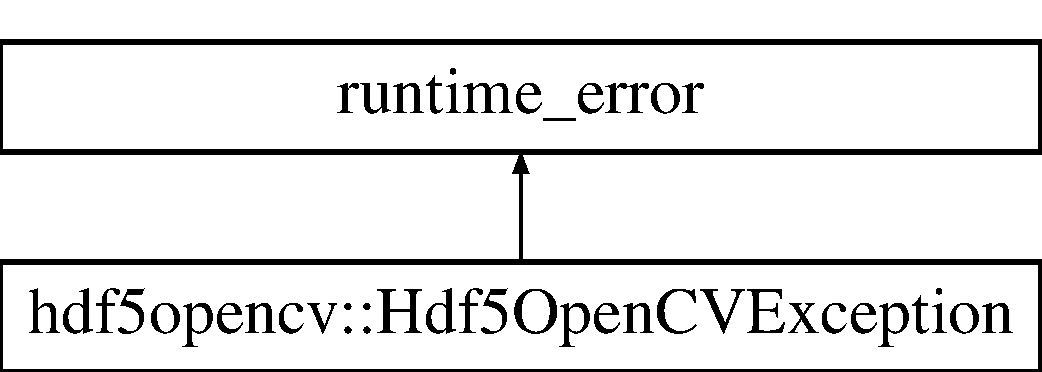
\includegraphics[height=2.000000cm]{classhdf5opencv_1_1_hdf5_open_c_v_exception}
\end{center}
\end{figure}
\subsection*{Public Member Functions}
\begin{DoxyCompactItemize}
\item 
\hyperlink{classhdf5opencv_1_1_hdf5_open_c_v_exception_a5faed3969b04be69294b9599327d5a51}{Hdf5\+Open\+C\+V\+Exception} (const std\+::string \&what\+\_\+arg)
\end{DoxyCompactItemize}


\subsection{Constructor \& Destructor Documentation}
\index{hdf5opencv\+::\+Hdf5\+Open\+C\+V\+Exception@{hdf5opencv\+::\+Hdf5\+Open\+C\+V\+Exception}!Hdf5\+Open\+C\+V\+Exception@{Hdf5\+Open\+C\+V\+Exception}}
\index{Hdf5\+Open\+C\+V\+Exception@{Hdf5\+Open\+C\+V\+Exception}!hdf5opencv\+::\+Hdf5\+Open\+C\+V\+Exception@{hdf5opencv\+::\+Hdf5\+Open\+C\+V\+Exception}}
\subsubsection[{\texorpdfstring{Hdf5\+Open\+C\+V\+Exception(const std\+::string \&what\+\_\+arg)}{Hdf5OpenCVException(const std::string &what_arg)}}]{\setlength{\rightskip}{0pt plus 5cm}hdf5opencv\+::\+Hdf5\+Open\+C\+V\+Exception\+::\+Hdf5\+Open\+C\+V\+Exception (
\begin{DoxyParamCaption}
\item[{const std\+::string \&}]{what\+\_\+arg}
\end{DoxyParamCaption}
)\hspace{0.3cm}{\ttfamily [inline]}}\hypertarget{classhdf5opencv_1_1_hdf5_open_c_v_exception_a5faed3969b04be69294b9599327d5a51}{}\label{classhdf5opencv_1_1_hdf5_open_c_v_exception_a5faed3969b04be69294b9599327d5a51}


The documentation for this class was generated from the following file\+:\begin{DoxyCompactItemize}
\item 
/home/stuermer/\+Repos/cpp/\+Echelle\+Simulator/include/\hyperlink{hdf5opencv_8h}{hdf5opencv.\+h}\end{DoxyCompactItemize}

\hypertarget{class_ideal_etalon}{}\section{Ideal\+Etalon Class Reference}
\label{class_ideal_etalon}\index{Ideal\+Etalon@{Ideal\+Etalon}}


Implements the spectral density of an ideal fabry-\/perot etalon.  




{\ttfamily \#include $<$source.\+h$>$}

Inheritance diagram for Ideal\+Etalon\+:\begin{figure}[H]
\begin{center}
\leavevmode
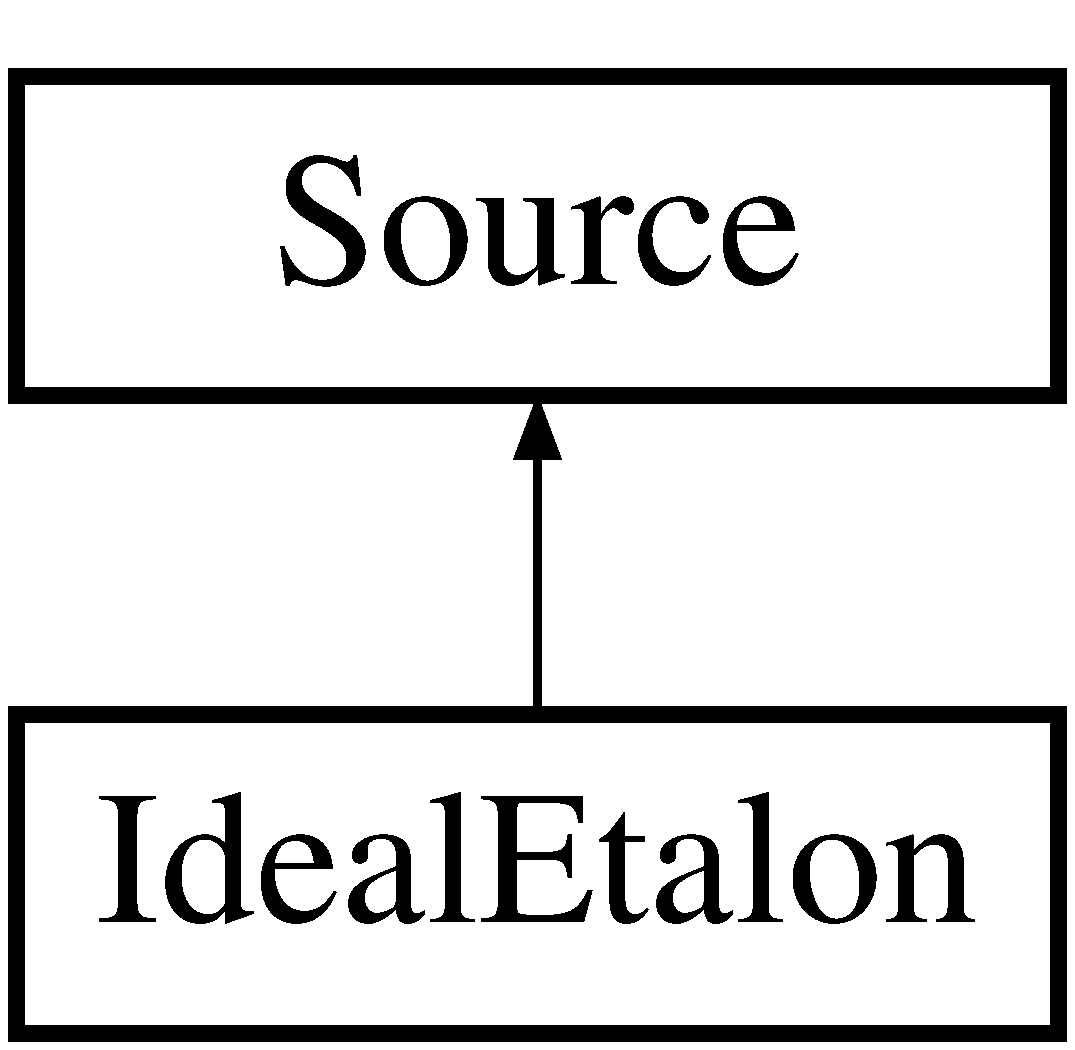
\includegraphics[height=2.000000cm]{class_ideal_etalon}
\end{center}
\end{figure}
\subsection*{Public Member Functions}
\begin{DoxyCompactItemize}
\item 
\hyperlink{class_ideal_etalon_acde8c0bcfe454c60177b00116ed5ae7e}{Ideal\+Etalon} (double \hyperlink{class_ideal_etalon_a8f63e477f8637502ef97b2f45875f57a}{d}, double \hyperlink{class_ideal_etalon_a1b1004d0898c3a054ca9cf412813c9d5}{n}, double \hyperlink{class_ideal_etalon_adb01dc93fb40a0735b5ed00907ffe0fd}{theta}, double \hyperlink{class_ideal_etalon_ae545946e739c8079c0ced7f836180cd1}{R})
\item 
double \hyperlink{class_ideal_etalon_a07e0545a681973d6be2e51e14a8945ef}{F\+SR} ()
\item 
double \hyperlink{class_ideal_etalon_a4b5547956e9795be364365e4997050c7}{F} ()
\item 
double \hyperlink{class_ideal_etalon_a6ba6c6d89e88e646da38ec45d12dab09}{get\+\_\+spectral\+\_\+density} (double wavelength)
\end{DoxyCompactItemize}
\subsection*{Static Public Member Functions}
\begin{DoxyCompactItemize}
\item 
static double \hyperlink{class_ideal_etalon_afc504294c3102f5a11de8cab99dc7943}{coefficient\+\_\+of\+\_\+finesse} (double \hyperlink{class_ideal_etalon_ae545946e739c8079c0ced7f836180cd1}{R})
\item 
static double \hyperlink{class_ideal_etalon_a18df1a0ca15f7d71763713f867cf3532}{T} (double wl, double \hyperlink{class_ideal_etalon_adb01dc93fb40a0735b5ed00907ffe0fd}{theta}, double \hyperlink{class_ideal_etalon_a8f63e477f8637502ef97b2f45875f57a}{d}, double \hyperlink{class_ideal_etalon_a1b1004d0898c3a054ca9cf412813c9d5}{n}, double \hyperlink{class_ideal_etalon_a93f909e0b51e64a057ac90985c5257fc}{cF})
\end{DoxyCompactItemize}
\subsection*{Private Attributes}
\begin{DoxyCompactItemize}
\item 
double \hyperlink{class_ideal_etalon_a8f63e477f8637502ef97b2f45875f57a}{d}
\item 
double \hyperlink{class_ideal_etalon_a1b1004d0898c3a054ca9cf412813c9d5}{n}
\item 
double \hyperlink{class_ideal_etalon_adb01dc93fb40a0735b5ed00907ffe0fd}{theta}
\item 
double \hyperlink{class_ideal_etalon_ae545946e739c8079c0ced7f836180cd1}{R}
\item 
double \hyperlink{class_ideal_etalon_a93f909e0b51e64a057ac90985c5257fc}{cF}
\end{DoxyCompactItemize}


\subsection{Detailed Description}
Implements the spectral density of an ideal fabry-\/perot etalon. 

An ideal Fabry-\/\+Perot etalon has a transmission function that only depends on the distance of the mirrors, the angle of incidence, the reflectivity of the mirrors and the refractive index of the medium between the mirrors. \[ s(\lambda) = \frac{1}{cF sin(\frac{\delta} {2})^2} \] (\begin{DoxySeeAlso}{See also}
\hyperlink{class_ideal_etalon_a18df1a0ca15f7d71763713f867cf3532}{Ideal\+Etalon\+::\+T()})
\end{DoxySeeAlso}
It produces a comb-\/like spectrum that is has equidistant peaks in frequency.

\begin{DoxyRefDesc}{Todo}
\item[\hyperlink{todo__todo000001}{Todo}]implement \hyperlink{class_ideal_etalon_a07e0545a681973d6be2e51e14a8945ef}{F\+S\+R()}, \hyperlink{class_ideal_etalon_a4b5547956e9795be364365e4997050c7}{F()} and other static functions.\end{DoxyRefDesc}


\subsection{Constructor \& Destructor Documentation}
\index{Ideal\+Etalon@{Ideal\+Etalon}!Ideal\+Etalon@{Ideal\+Etalon}}
\index{Ideal\+Etalon@{Ideal\+Etalon}!Ideal\+Etalon@{Ideal\+Etalon}}
\subsubsection[{\texorpdfstring{Ideal\+Etalon(double d, double n, double theta, double R)}{IdealEtalon(double d, double n, double theta, double R)}}]{\setlength{\rightskip}{0pt plus 5cm}Ideal\+Etalon\+::\+Ideal\+Etalon (
\begin{DoxyParamCaption}
\item[{double}]{d, }
\item[{double}]{n, }
\item[{double}]{theta, }
\item[{double}]{R}
\end{DoxyParamCaption}
)}\hypertarget{class_ideal_etalon_acde8c0bcfe454c60177b00116ed5ae7e}{}\label{class_ideal_etalon_acde8c0bcfe454c60177b00116ed5ae7e}
Constructor.


\begin{DoxyParams}{Parameters}
{\em d} & mirror distance in mm \\
\hline
{\em n} & refractive index of the medium between mirrors \\
\hline
{\em theta} & angle of incidence \\
\hline
{\em R} & reflectivity of the mirrors \\
\hline
\end{DoxyParams}


\subsection{Member Function Documentation}
\index{Ideal\+Etalon@{Ideal\+Etalon}!coefficient\+\_\+of\+\_\+finesse@{coefficient\+\_\+of\+\_\+finesse}}
\index{coefficient\+\_\+of\+\_\+finesse@{coefficient\+\_\+of\+\_\+finesse}!Ideal\+Etalon@{Ideal\+Etalon}}
\subsubsection[{\texorpdfstring{coefficient\+\_\+of\+\_\+finesse(double R)}{coefficient_of_finesse(double R)}}]{\setlength{\rightskip}{0pt plus 5cm}double Ideal\+Etalon\+::coefficient\+\_\+of\+\_\+finesse (
\begin{DoxyParamCaption}
\item[{double}]{R}
\end{DoxyParamCaption}
)\hspace{0.3cm}{\ttfamily [static]}}\hypertarget{class_ideal_etalon_afc504294c3102f5a11de8cab99dc7943}{}\label{class_ideal_etalon_afc504294c3102f5a11de8cab99dc7943}
Calculates the coefficient of Finesse.

\[ cF = \frac{4 R}{(1-R)^2} \]

\begin{DoxyWarning}{Warning}
This is not what is typically called the finesse of an etalon, but the coefficient of finesse.
\end{DoxyWarning}

\begin{DoxyParams}{Parameters}
{\em R} & mirror reflectivity \\
\hline
\end{DoxyParams}
\begin{DoxyReturn}{Returns}
coefficienct of finesse 
\end{DoxyReturn}
\index{Ideal\+Etalon@{Ideal\+Etalon}!F@{F}}
\index{F@{F}!Ideal\+Etalon@{Ideal\+Etalon}}
\subsubsection[{\texorpdfstring{F()}{F()}}]{\setlength{\rightskip}{0pt plus 5cm}double Ideal\+Etalon\+::F (
\begin{DoxyParamCaption}
{}
\end{DoxyParamCaption}
)}\hypertarget{class_ideal_etalon_a4b5547956e9795be364365e4997050c7}{}\label{class_ideal_etalon_a4b5547956e9795be364365e4997050c7}
\index{Ideal\+Etalon@{Ideal\+Etalon}!F\+SR@{F\+SR}}
\index{F\+SR@{F\+SR}!Ideal\+Etalon@{Ideal\+Etalon}}
\subsubsection[{\texorpdfstring{F\+S\+R()}{FSR()}}]{\setlength{\rightskip}{0pt plus 5cm}double Ideal\+Etalon\+::\+F\+SR (
\begin{DoxyParamCaption}
{}
\end{DoxyParamCaption}
)}\hypertarget{class_ideal_etalon_a07e0545a681973d6be2e51e14a8945ef}{}\label{class_ideal_etalon_a07e0545a681973d6be2e51e14a8945ef}
\index{Ideal\+Etalon@{Ideal\+Etalon}!get\+\_\+spectral\+\_\+density@{get\+\_\+spectral\+\_\+density}}
\index{get\+\_\+spectral\+\_\+density@{get\+\_\+spectral\+\_\+density}!Ideal\+Etalon@{Ideal\+Etalon}}
\subsubsection[{\texorpdfstring{get\+\_\+spectral\+\_\+density(double wavelength)}{get_spectral_density(double wavelength)}}]{\setlength{\rightskip}{0pt plus 5cm}double Ideal\+Etalon\+::get\+\_\+spectral\+\_\+density (
\begin{DoxyParamCaption}
\item[{double}]{wavelength}
\end{DoxyParamCaption}
)\hspace{0.3cm}{\ttfamily [virtual]}}\hypertarget{class_ideal_etalon_a6ba6c6d89e88e646da38ec45d12dab09}{}\label{class_ideal_etalon_a6ba6c6d89e88e646da38ec45d12dab09}
Spectral density at given wavelegnth.


\begin{DoxyParams}{Parameters}
{\em wavelength} & wavelength \mbox{[}micron\mbox{]} \\
\hline
\end{DoxyParams}
\begin{DoxyReturn}{Returns}
Spectral density at given wavelength 
\end{DoxyReturn}


Reimplemented from \hyperlink{class_source_a546ae8ec1ae47e888c74f146278e19af}{Source}.

\index{Ideal\+Etalon@{Ideal\+Etalon}!T@{T}}
\index{T@{T}!Ideal\+Etalon@{Ideal\+Etalon}}
\subsubsection[{\texorpdfstring{T(double wl, double theta, double d, double n, double c\+F)}{T(double wl, double theta, double d, double n, double cF)}}]{\setlength{\rightskip}{0pt plus 5cm}double Ideal\+Etalon\+::T (
\begin{DoxyParamCaption}
\item[{double}]{wl, }
\item[{double}]{theta, }
\item[{double}]{d, }
\item[{double}]{n, }
\item[{double}]{cF}
\end{DoxyParamCaption}
)\hspace{0.3cm}{\ttfamily [static]}}\hypertarget{class_ideal_etalon_a18df1a0ca15f7d71763713f867cf3532}{}\label{class_ideal_etalon_a18df1a0ca15f7d71763713f867cf3532}
Transmission function of an ideal etalon. \[ T(\lambda) = \frac{1}{cF sin(\frac{\delta} {2})^2} \], where \[ \delta \left( \frac{2\pi}{\lambda} \right) 2nlcos(\Theta) \], is the phase difference and $ F $ is the coefficient of finesse\+: \[ cF = \frac{4R}{(1-R)^2} \]


\begin{DoxyParams}{Parameters}
{\em wl} & wavelength \mbox{[}micron\mbox{]} \\
\hline
{\em theta} & angle of incidence \mbox{[}rad\mbox{]} \\
\hline
{\em d} & mirror distance \mbox{[}mm\mbox{]} \\
\hline
{\em n} & refractive index \\
\hline
{\em cF} & coefficient of finesse \\
\hline
\end{DoxyParams}
\begin{DoxySeeAlso}{See also}
\hyperlink{class_ideal_etalon_afc504294c3102f5a11de8cab99dc7943}{Ideal\+Etalon\+::coefficient\+\_\+of\+\_\+finesse} 
\end{DoxySeeAlso}
\begin{DoxyReturn}{Returns}
transmission at given wavelength 
\end{DoxyReturn}


\subsection{Member Data Documentation}
\index{Ideal\+Etalon@{Ideal\+Etalon}!cF@{cF}}
\index{cF@{cF}!Ideal\+Etalon@{Ideal\+Etalon}}
\subsubsection[{\texorpdfstring{cF}{cF}}]{\setlength{\rightskip}{0pt plus 5cm}double Ideal\+Etalon\+::cF\hspace{0.3cm}{\ttfamily [private]}}\hypertarget{class_ideal_etalon_a93f909e0b51e64a057ac90985c5257fc}{}\label{class_ideal_etalon_a93f909e0b51e64a057ac90985c5257fc}
\index{Ideal\+Etalon@{Ideal\+Etalon}!d@{d}}
\index{d@{d}!Ideal\+Etalon@{Ideal\+Etalon}}
\subsubsection[{\texorpdfstring{d}{d}}]{\setlength{\rightskip}{0pt plus 5cm}double Ideal\+Etalon\+::d\hspace{0.3cm}{\ttfamily [private]}}\hypertarget{class_ideal_etalon_a8f63e477f8637502ef97b2f45875f57a}{}\label{class_ideal_etalon_a8f63e477f8637502ef97b2f45875f57a}
\index{Ideal\+Etalon@{Ideal\+Etalon}!n@{n}}
\index{n@{n}!Ideal\+Etalon@{Ideal\+Etalon}}
\subsubsection[{\texorpdfstring{n}{n}}]{\setlength{\rightskip}{0pt plus 5cm}double Ideal\+Etalon\+::n\hspace{0.3cm}{\ttfamily [private]}}\hypertarget{class_ideal_etalon_a1b1004d0898c3a054ca9cf412813c9d5}{}\label{class_ideal_etalon_a1b1004d0898c3a054ca9cf412813c9d5}
\index{Ideal\+Etalon@{Ideal\+Etalon}!R@{R}}
\index{R@{R}!Ideal\+Etalon@{Ideal\+Etalon}}
\subsubsection[{\texorpdfstring{R}{R}}]{\setlength{\rightskip}{0pt plus 5cm}double Ideal\+Etalon\+::R\hspace{0.3cm}{\ttfamily [private]}}\hypertarget{class_ideal_etalon_ae545946e739c8079c0ced7f836180cd1}{}\label{class_ideal_etalon_ae545946e739c8079c0ced7f836180cd1}
\index{Ideal\+Etalon@{Ideal\+Etalon}!theta@{theta}}
\index{theta@{theta}!Ideal\+Etalon@{Ideal\+Etalon}}
\subsubsection[{\texorpdfstring{theta}{theta}}]{\setlength{\rightskip}{0pt plus 5cm}double Ideal\+Etalon\+::theta\hspace{0.3cm}{\ttfamily [private]}}\hypertarget{class_ideal_etalon_adb01dc93fb40a0735b5ed00907ffe0fd}{}\label{class_ideal_etalon_adb01dc93fb40a0735b5ed00907ffe0fd}


The documentation for this class was generated from the following files\+:\begin{DoxyCompactItemize}
\item 
/home/stuermer/\+Repos/cpp/\+Echelle\+Simulator/include/\hyperlink{source_8h}{source.\+h}\item 
/home/stuermer/\+Repos/cpp/\+Echelle\+Simulator/src/\hyperlink{source_8cpp}{source.\+cpp}\end{DoxyCompactItemize}

\hypertarget{class_line_list}{}\section{Line\+List Class Reference}
\label{class_line_list}\index{Line\+List@{Line\+List}}


Implements line list spectrum.  




{\ttfamily \#include $<$source.\+h$>$}

Inheritance diagram for Line\+List\+:\begin{figure}[H]
\begin{center}
\leavevmode
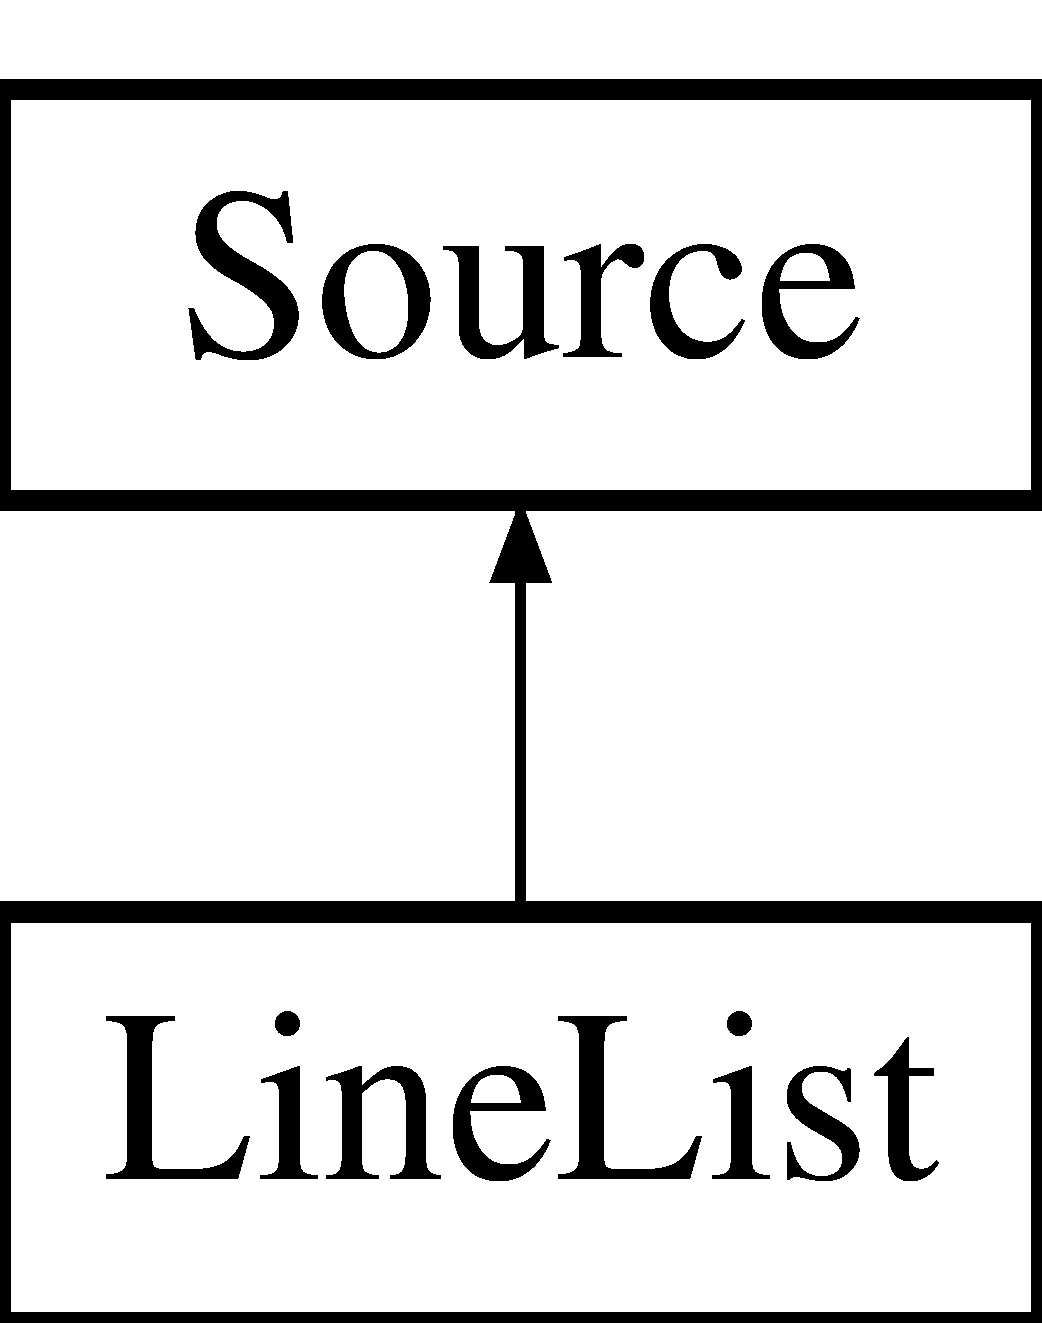
\includegraphics[height=2.000000cm]{class_line_list}
\end{center}
\end{figure}
\subsection*{Public Member Functions}
\begin{DoxyCompactItemize}
\item 
\hyperlink{class_line_list_aa2d1b522deec10a431ad6eacc4c614fd}{Line\+List} (std\+::string linelist)
\item 
void \hyperlink{class_line_list_a24602f1ed3e346d6c06e788d00dae6e8}{read\+\_\+spectrum} (std\+::string linelist)
\item 
double \hyperlink{class_line_list_acb1e41d6120cf6bc0df2afaeb35a5aad}{get\+\_\+spectral\+\_\+density} (double wavelength)
\item 
std\+::vector$<$ double $>$ \hyperlink{class_line_list_aa51704a60f48389c06c583d2a4cc6733}{get\+\_\+spectrum} (std\+::vector$<$ double $>$ wavelength)
\item 
std\+::vector$<$ double $>$ \hyperlink{class_line_list_acfc2f92ac90099e4d4a2d3f2fcac47ef}{get\+\_\+wavelength} ()
\end{DoxyCompactItemize}
\subsection*{Private Attributes}
\begin{DoxyCompactItemize}
\item 
std\+::map$<$ double, double $>$ \hyperlink{class_line_list_af8d4ea58795d9cc4687a21884f2953b3}{data}
\end{DoxyCompactItemize}


\subsection{Detailed Description}
Implements line list spectrum. 

\subsection{Constructor \& Destructor Documentation}
\index{Line\+List@{Line\+List}!Line\+List@{Line\+List}}
\index{Line\+List@{Line\+List}!Line\+List@{Line\+List}}
\subsubsection[{\texorpdfstring{Line\+List(std\+::string linelist)}{LineList(std::string linelist)}}]{\setlength{\rightskip}{0pt plus 5cm}Line\+List\+::\+Line\+List (
\begin{DoxyParamCaption}
\item[{std\+::string}]{linelist}
\end{DoxyParamCaption}
)}\hypertarget{class_line_list_aa2d1b522deec10a431ad6eacc4c614fd}{}\label{class_line_list_aa2d1b522deec10a431ad6eacc4c614fd}


\subsection{Member Function Documentation}
\index{Line\+List@{Line\+List}!get\+\_\+spectral\+\_\+density@{get\+\_\+spectral\+\_\+density}}
\index{get\+\_\+spectral\+\_\+density@{get\+\_\+spectral\+\_\+density}!Line\+List@{Line\+List}}
\subsubsection[{\texorpdfstring{get\+\_\+spectral\+\_\+density(double wavelength)}{get_spectral_density(double wavelength)}}]{\setlength{\rightskip}{0pt plus 5cm}double Line\+List\+::get\+\_\+spectral\+\_\+density (
\begin{DoxyParamCaption}
\item[{double}]{wavelength}
\end{DoxyParamCaption}
)\hspace{0.3cm}{\ttfamily [virtual]}}\hypertarget{class_line_list_acb1e41d6120cf6bc0df2afaeb35a5aad}{}\label{class_line_list_acb1e41d6120cf6bc0df2afaeb35a5aad}
This function returns the spectral density at a given wavelength. It is the essential function for all subclasses. \begin{DoxySeeAlso}{See also}
\hyperlink{class_source_ab5d90ab3a4cfb8403803d88ce8b9f0f8}{Source\+::get\+\_\+spectrum()} will use this function to integrate over it to retreive a spectrum for a given wavelength vector. 
\end{DoxySeeAlso}

\begin{DoxyParams}{Parameters}
{\em wavelength} & wavelength \\
\hline
\end{DoxyParams}
\begin{DoxyReturn}{Returns}
spectral density 
\end{DoxyReturn}


Reimplemented from \hyperlink{class_source_a546ae8ec1ae47e888c74f146278e19af}{Source}.

\index{Line\+List@{Line\+List}!get\+\_\+spectrum@{get\+\_\+spectrum}}
\index{get\+\_\+spectrum@{get\+\_\+spectrum}!Line\+List@{Line\+List}}
\subsubsection[{\texorpdfstring{get\+\_\+spectrum(std\+::vector$<$ double $>$ wavelength)}{get_spectrum(std::vector< double > wavelength)}}]{\setlength{\rightskip}{0pt plus 5cm}std\+::vector$<$ double $>$ Line\+List\+::get\+\_\+spectrum (
\begin{DoxyParamCaption}
\item[{std\+::vector$<$ double $>$}]{wavelength}
\end{DoxyParamCaption}
)\hspace{0.3cm}{\ttfamily [virtual]}}\hypertarget{class_line_list_aa51704a60f48389c06c583d2a4cc6733}{}\label{class_line_list_aa51704a60f48389c06c583d2a4cc6733}
Returns spectrum at given wavelength

This function returns the integrated spectral density for a given wavelength vector. 
\begin{DoxyParams}{Parameters}
{\em wavelength} & wavelength vector \\
\hline
\end{DoxyParams}
\begin{DoxyReturn}{Returns}
spectrum at given wavelength 
\end{DoxyReturn}


Reimplemented from \hyperlink{class_source_ab5d90ab3a4cfb8403803d88ce8b9f0f8}{Source}.

\index{Line\+List@{Line\+List}!get\+\_\+wavelength@{get\+\_\+wavelength}}
\index{get\+\_\+wavelength@{get\+\_\+wavelength}!Line\+List@{Line\+List}}
\subsubsection[{\texorpdfstring{get\+\_\+wavelength()}{get_wavelength()}}]{\setlength{\rightskip}{0pt plus 5cm}std\+::vector$<$ double $>$ Line\+List\+::get\+\_\+wavelength (
\begin{DoxyParamCaption}
{}
\end{DoxyParamCaption}
)}\hypertarget{class_line_list_acfc2f92ac90099e4d4a2d3f2fcac47ef}{}\label{class_line_list_acfc2f92ac90099e4d4a2d3f2fcac47ef}
\index{Line\+List@{Line\+List}!read\+\_\+spectrum@{read\+\_\+spectrum}}
\index{read\+\_\+spectrum@{read\+\_\+spectrum}!Line\+List@{Line\+List}}
\subsubsection[{\texorpdfstring{read\+\_\+spectrum(std\+::string linelist)}{read_spectrum(std::string linelist)}}]{\setlength{\rightskip}{0pt plus 5cm}void Line\+List\+::read\+\_\+spectrum (
\begin{DoxyParamCaption}
\item[{std\+::string}]{linelist}
\end{DoxyParamCaption}
)}\hypertarget{class_line_list_a24602f1ed3e346d6c06e788d00dae6e8}{}\label{class_line_list_a24602f1ed3e346d6c06e788d00dae6e8}


\subsection{Member Data Documentation}
\index{Line\+List@{Line\+List}!data@{data}}
\index{data@{data}!Line\+List@{Line\+List}}
\subsubsection[{\texorpdfstring{data}{data}}]{\setlength{\rightskip}{0pt plus 5cm}std\+::map$<$double, double$>$ Line\+List\+::data\hspace{0.3cm}{\ttfamily [private]}}\hypertarget{class_line_list_af8d4ea58795d9cc4687a21884f2953b3}{}\label{class_line_list_af8d4ea58795d9cc4687a21884f2953b3}


The documentation for this class was generated from the following files\+:\begin{DoxyCompactItemize}
\item 
/home/stuermer/\+Repos/cpp/\+Echelle\+Simulator/include/\hyperlink{source_8h}{source.\+h}\item 
/home/stuermer/\+Repos/cpp/\+Echelle\+Simulator/src/\hyperlink{source_8cpp}{source.\+cpp}\end{DoxyCompactItemize}

\hypertarget{class_matrix_simulator}{}\section{Matrix\+Simulator Class Reference}
\label{class_matrix_simulator}\index{Matrix\+Simulator@{Matrix\+Simulator}}


{\ttfamily \#include $<$matrixsimulator.\+h$>$}

\subsection*{Public Member Functions}
\begin{DoxyCompactItemize}
\item 
\hyperlink{class_matrix_simulator_ae3feb47ab98f917ad0b8b4b53d1b34aa}{Matrix\+Simulator} ()
\item 
void \hyperlink{class_matrix_simulator_a7d6123f82db49f9054228c31ba5dd44e}{read\+\_\+transformations} (std\+::string path)
\item 
cv\+::\+Mat \hyperlink{class_matrix_simulator_a5bdb033cbabf36fdd7f57a92f65dbec6}{get\+\_\+transformation\+\_\+matrix} (int order, double wavelength)
\item 
void \hyperlink{class_matrix_simulator_aa584302cfbfc8d5f02f184282bd60584}{calc\+\_\+splines} ()
\item 
void \hyperlink{class_matrix_simulator_a516c57a6e2d27e249202c60bd0fb5cc6}{set\+\_\+wavelength} (int N)
\item 
void \hyperlink{class_matrix_simulator_a85e8651b0a540ae40b3352ee73ed1c11}{set\+\_\+wavelength} (std\+::vector$<$ double $>$ wavelength)
\item 
void \hyperlink{class_matrix_simulator_a225df602310e87aa476faafafb08bb48}{calc\+\_\+sim\+\_\+matrices} ()
\item 
cv\+::\+Mat \hyperlink{class_matrix_simulator_a3016ecb082ba87ef7594928c14d74694}{transform\+\_\+slit} (cv\+::\+Mat \&slit\+\_\+image, cv\+::\+Mat \&transformation\+\_\+matrix, double weight)
\item 
int \hyperlink{class_matrix_simulator_a48920e35ea386faca140453878c4ed38}{simulate\+\_\+order} (int order, cv\+::\+Mat \&slit\+\_\+image, cv\+::\+Mat \&output\+\_\+image, bool aberrations)
\item 
void \hyperlink{class_matrix_simulator_a92cbe25d3d5317dac8ded3d974710bbd}{simulate\+\_\+spectrum} ()
\item 
void \hyperlink{class_matrix_simulator_aed5d9befa4e4c4af5e6331a836d25e6c}{set\+\_\+efficiencies} (std\+::vector$<$ \hyperlink{class_efficiency}{Efficiency} $\ast$ $>$ \&\hyperlink{class_matrix_simulator_a05c00fb5164a5faa987da2642b899035}{efficiencies})
\item 
void \hyperlink{class_matrix_simulator_a2caa7f889603addf02db9094c20b91a6}{add\+\_\+efficiency} (\hyperlink{class_efficiency}{Efficiency} $\ast$eff)
\item 
void \hyperlink{class_matrix_simulator_a250a81596cd303057c4d14a86c4bb728}{add\+\_\+source} (\hyperlink{class_source}{Source} $\ast$src)
\item 
void \hyperlink{class_matrix_simulator_a9a9afb06c7285f20658092da61f65c36}{load\+\_\+spectrograph\+\_\+model} (std\+::string path, int fiber\+\_\+number)
\item 
void \hyperlink{class_matrix_simulator_a26d15d1dd2e1e8944e74e5f9f47dca76}{set\+\_\+order\+\_\+range} (int min\+\_\+order, int max\+\_\+order)
\item 
void \hyperlink{class_matrix_simulator_a0741978f171e1c5f229c19de64042958}{set\+\_\+ccd} (\hyperlink{class_c_c_d}{C\+CD} $\ast$\hyperlink{class_matrix_simulator_a151ec381d921be1b5b30fef6430ceb91}{ccd})
\item 
void \hyperlink{class_matrix_simulator_afaf8acf533e2b0e0e440aabbeb6a4743}{set\+\_\+slit} (\hyperlink{class_slit}{Slit} $\ast$\hyperlink{class_matrix_simulator_a5b054ede1af3c6e29296af6f2cd5e313}{slit})
\item 
void \hyperlink{class_matrix_simulator_ad31531aec0901325d6e01ebbd82b1da5}{set\+\_\+psfs} (\hyperlink{class_p_s_f}{P\+SF} $\ast$\hyperlink{class_matrix_simulator_a4f8b1a0772c43203f1b06420c0d018fa}{psfs})
\item 
void \hyperlink{class_matrix_simulator_a042e798c6f289100c88a656f71101502}{prepare\+\_\+sources} (std\+::vector$<$ \hyperlink{class_source}{Source} $\ast$ $>$ \hyperlink{class_matrix_simulator_abb3bc16d0336f6bbda99300ceccdf427}{sources})
\item 
void \hyperlink{class_matrix_simulator_ac7e48c2e271c13b09e5a1c55f6f477c8}{save\+\_\+to\+\_\+file} (std\+::string filename, bool downsample=true, bool bleed=true, bool overwrite=false)
\item 
void \hyperlink{class_matrix_simulator_a8ce41368c573f2faba7e74a5756250e4}{transformation\+\_\+to\+\_\+file} (std\+::string filename)
\item 
double \hyperlink{class_matrix_simulator_abf10a6ad60e8fa959e41df6a1f07c82d}{get\+\_\+blaze} ()
\item 
double \hyperlink{class_matrix_simulator_ab4e1e824d0e819fcf967d7d8b770de8a}{get\+\_\+gpmm} ()
\end{DoxyCompactItemize}
\subsection*{Public Attributes}
\begin{DoxyCompactItemize}
\item 
std\+::vector$<$ int $>$ \hyperlink{class_matrix_simulator_a5524a9a77d30e2b396737260ec6f73f8}{orders}
\item 
int \hyperlink{class_matrix_simulator_a2da306f4e998a609e9a9f26688d80949}{raw\+\_\+n}
\item 
\hyperlink{class_c_c_d}{C\+CD} $\ast$ \hyperlink{class_matrix_simulator_a151ec381d921be1b5b30fef6430ceb91}{ccd}
\end{DoxyCompactItemize}
\subsection*{Private Attributes}
\begin{DoxyCompactItemize}
\item 
cv\+::\+Mat \hyperlink{class_matrix_simulator_a90bcc13f784a69c54ad605ef77dcbbe8}{img}
\item 
std\+::map$<$ int, std\+::vector$<$ \hyperlink{structraw__transformation}{raw\+\_\+transformation} $>$ $>$ \hyperlink{class_matrix_simulator_a1266c67228a0fc2c1387c4e7454fe435}{raw\+\_\+transformations}
\item 
std\+::vector$<$ \hyperlink{class_efficiency}{Efficiency} $\ast$ $>$ \hyperlink{class_matrix_simulator_a05c00fb5164a5faa987da2642b899035}{efficiencies}
\item 
std\+::vector$<$ \hyperlink{class_source}{Source} $\ast$ $>$ \hyperlink{class_matrix_simulator_abb3bc16d0336f6bbda99300ceccdf427}{sources}
\item 
std\+::map$<$ int, std\+::vector$<$ double $>$ $>$ \hyperlink{class_matrix_simulator_aac8850d4461c6a7775dc44f6bdafb2e2}{sim\+\_\+wavelength}
\item 
std\+::map$<$ int, std\+::vector$<$ cv\+::\+Mat $>$ $>$ \hyperlink{class_matrix_simulator_a4886dd70ef084bd73bb224c7f28897ee}{sim\+\_\+matrices}
\item 
std\+::map$<$ int, std\+::vector$<$ double $>$ $>$ \hyperlink{class_matrix_simulator_a6202de105f6c949a226b98bb048560c1}{sim\+\_\+efficiencies}
\item 
std\+::map$<$ int, std\+::vector$<$ double $>$ $>$ \hyperlink{class_matrix_simulator_aa3ddf31246c9f2be64ab12fe4b47e8af}{sim\+\_\+spectra}
\item 
std\+::map$<$ int, tk\+::spline $>$ \hyperlink{class_matrix_simulator_a8f9852337a1ab80f532ff69ae2b41b3b}{tr\+\_\+p}
\item 
std\+::map$<$ int, tk\+::spline $>$ \hyperlink{class_matrix_simulator_a52d4a39c875373d76c0f7b9baf5f1e2f}{tr\+\_\+r}
\item 
std\+::map$<$ int, tk\+::spline $>$ \hyperlink{class_matrix_simulator_a18bb49a4ca4363acce7e33382d578edb}{tr\+\_\+q}
\item 
std\+::map$<$ int, tk\+::spline $>$ \hyperlink{class_matrix_simulator_ac892d19d1c68c6414b9a3c999205092b}{tr\+\_\+phi}
\item 
std\+::map$<$ int, tk\+::spline $>$ \hyperlink{class_matrix_simulator_aa544354356e00fe4da0edcb30f37e6b4}{tr\+\_\+tx}
\item 
std\+::map$<$ int, tk\+::spline $>$ \hyperlink{class_matrix_simulator_a3d7f3962f4b2d2de111bc00539e0ba68}{tr\+\_\+ty}
\item 
\hyperlink{class_p_s_f}{P\+SF} $\ast$ \hyperlink{class_matrix_simulator_a4f8b1a0772c43203f1b06420c0d018fa}{psfs}
\item 
\hyperlink{class_slit}{Slit} $\ast$ \hyperlink{class_matrix_simulator_a5b054ede1af3c6e29296af6f2cd5e313}{slit}
\item 
\hyperlink{structspectrograph__information}{spectrograph\+\_\+information} \hyperlink{class_matrix_simulator_a3a1e3511ea01199d625b19f4add87b75}{spec\+\_\+info}
\end{DoxyCompactItemize}


\subsection{Constructor \& Destructor Documentation}
\index{Matrix\+Simulator@{Matrix\+Simulator}!Matrix\+Simulator@{Matrix\+Simulator}}
\index{Matrix\+Simulator@{Matrix\+Simulator}!Matrix\+Simulator@{Matrix\+Simulator}}
\subsubsection[{\texorpdfstring{Matrix\+Simulator()}{MatrixSimulator()}}]{\setlength{\rightskip}{0pt plus 5cm}Matrix\+Simulator\+::\+Matrix\+Simulator (
\begin{DoxyParamCaption}
{}
\end{DoxyParamCaption}
)}\hypertarget{class_matrix_simulator_ae3feb47ab98f917ad0b8b4b53d1b34aa}{}\label{class_matrix_simulator_ae3feb47ab98f917ad0b8b4b53d1b34aa}


\subsection{Member Function Documentation}
\index{Matrix\+Simulator@{Matrix\+Simulator}!add\+\_\+efficiency@{add\+\_\+efficiency}}
\index{add\+\_\+efficiency@{add\+\_\+efficiency}!Matrix\+Simulator@{Matrix\+Simulator}}
\subsubsection[{\texorpdfstring{add\+\_\+efficiency(\+Efficiency $\ast$eff)}{add_efficiency(Efficiency *eff)}}]{\setlength{\rightskip}{0pt plus 5cm}void Matrix\+Simulator\+::add\+\_\+efficiency (
\begin{DoxyParamCaption}
\item[{{\bf Efficiency} $\ast$}]{eff}
\end{DoxyParamCaption}
)}\hypertarget{class_matrix_simulator_a2caa7f889603addf02db9094c20b91a6}{}\label{class_matrix_simulator_a2caa7f889603addf02db9094c20b91a6}
\index{Matrix\+Simulator@{Matrix\+Simulator}!add\+\_\+source@{add\+\_\+source}}
\index{add\+\_\+source@{add\+\_\+source}!Matrix\+Simulator@{Matrix\+Simulator}}
\subsubsection[{\texorpdfstring{add\+\_\+source(\+Source $\ast$src)}{add_source(Source *src)}}]{\setlength{\rightskip}{0pt plus 5cm}void Matrix\+Simulator\+::add\+\_\+source (
\begin{DoxyParamCaption}
\item[{{\bf Source} $\ast$}]{src}
\end{DoxyParamCaption}
)}\hypertarget{class_matrix_simulator_a250a81596cd303057c4d14a86c4bb728}{}\label{class_matrix_simulator_a250a81596cd303057c4d14a86c4bb728}
\index{Matrix\+Simulator@{Matrix\+Simulator}!calc\+\_\+sim\+\_\+matrices@{calc\+\_\+sim\+\_\+matrices}}
\index{calc\+\_\+sim\+\_\+matrices@{calc\+\_\+sim\+\_\+matrices}!Matrix\+Simulator@{Matrix\+Simulator}}
\subsubsection[{\texorpdfstring{calc\+\_\+sim\+\_\+matrices()}{calc_sim_matrices()}}]{\setlength{\rightskip}{0pt plus 5cm}void Matrix\+Simulator\+::calc\+\_\+sim\+\_\+matrices (
\begin{DoxyParamCaption}
{}
\end{DoxyParamCaption}
)}\hypertarget{class_matrix_simulator_a225df602310e87aa476faafafb08bb48}{}\label{class_matrix_simulator_a225df602310e87aa476faafafb08bb48}
\index{Matrix\+Simulator@{Matrix\+Simulator}!calc\+\_\+splines@{calc\+\_\+splines}}
\index{calc\+\_\+splines@{calc\+\_\+splines}!Matrix\+Simulator@{Matrix\+Simulator}}
\subsubsection[{\texorpdfstring{calc\+\_\+splines()}{calc_splines()}}]{\setlength{\rightskip}{0pt plus 5cm}void Matrix\+Simulator\+::calc\+\_\+splines (
\begin{DoxyParamCaption}
{}
\end{DoxyParamCaption}
)}\hypertarget{class_matrix_simulator_aa584302cfbfc8d5f02f184282bd60584}{}\label{class_matrix_simulator_aa584302cfbfc8d5f02f184282bd60584}
\index{Matrix\+Simulator@{Matrix\+Simulator}!get\+\_\+blaze@{get\+\_\+blaze}}
\index{get\+\_\+blaze@{get\+\_\+blaze}!Matrix\+Simulator@{Matrix\+Simulator}}
\subsubsection[{\texorpdfstring{get\+\_\+blaze()}{get_blaze()}}]{\setlength{\rightskip}{0pt plus 5cm}double Matrix\+Simulator\+::get\+\_\+blaze (
\begin{DoxyParamCaption}
{}
\end{DoxyParamCaption}
)}\hypertarget{class_matrix_simulator_abf10a6ad60e8fa959e41df6a1f07c82d}{}\label{class_matrix_simulator_abf10a6ad60e8fa959e41df6a1f07c82d}
\index{Matrix\+Simulator@{Matrix\+Simulator}!get\+\_\+gpmm@{get\+\_\+gpmm}}
\index{get\+\_\+gpmm@{get\+\_\+gpmm}!Matrix\+Simulator@{Matrix\+Simulator}}
\subsubsection[{\texorpdfstring{get\+\_\+gpmm()}{get_gpmm()}}]{\setlength{\rightskip}{0pt plus 5cm}double Matrix\+Simulator\+::get\+\_\+gpmm (
\begin{DoxyParamCaption}
{}
\end{DoxyParamCaption}
)}\hypertarget{class_matrix_simulator_ab4e1e824d0e819fcf967d7d8b770de8a}{}\label{class_matrix_simulator_ab4e1e824d0e819fcf967d7d8b770de8a}
\index{Matrix\+Simulator@{Matrix\+Simulator}!get\+\_\+transformation\+\_\+matrix@{get\+\_\+transformation\+\_\+matrix}}
\index{get\+\_\+transformation\+\_\+matrix@{get\+\_\+transformation\+\_\+matrix}!Matrix\+Simulator@{Matrix\+Simulator}}
\subsubsection[{\texorpdfstring{get\+\_\+transformation\+\_\+matrix(int order, double wavelength)}{get_transformation_matrix(int order, double wavelength)}}]{\setlength{\rightskip}{0pt plus 5cm}cv\+::\+Mat Matrix\+Simulator\+::get\+\_\+transformation\+\_\+matrix (
\begin{DoxyParamCaption}
\item[{int}]{order, }
\item[{double}]{wavelength}
\end{DoxyParamCaption}
)}\hypertarget{class_matrix_simulator_a5bdb033cbabf36fdd7f57a92f65dbec6}{}\label{class_matrix_simulator_a5bdb033cbabf36fdd7f57a92f65dbec6}
\index{Matrix\+Simulator@{Matrix\+Simulator}!load\+\_\+spectrograph\+\_\+model@{load\+\_\+spectrograph\+\_\+model}}
\index{load\+\_\+spectrograph\+\_\+model@{load\+\_\+spectrograph\+\_\+model}!Matrix\+Simulator@{Matrix\+Simulator}}
\subsubsection[{\texorpdfstring{load\+\_\+spectrograph\+\_\+model(std\+::string path, int fiber\+\_\+number)}{load_spectrograph_model(std::string path, int fiber_number)}}]{\setlength{\rightskip}{0pt plus 5cm}void Matrix\+Simulator\+::load\+\_\+spectrograph\+\_\+model (
\begin{DoxyParamCaption}
\item[{std\+::string}]{path, }
\item[{int}]{fiber\+\_\+number}
\end{DoxyParamCaption}
)}\hypertarget{class_matrix_simulator_a9a9afb06c7285f20658092da61f65c36}{}\label{class_matrix_simulator_a9a9afb06c7285f20658092da61f65c36}
Load spectrograph model from H\+DF file 
\begin{DoxyParams}{Parameters}
{\em path} & path to H\+DF file containing spectrograph model \\
\hline
{\em fiber\+\_\+number} & fiber to select \\
\hline
\end{DoxyParams}
\index{Matrix\+Simulator@{Matrix\+Simulator}!prepare\+\_\+sources@{prepare\+\_\+sources}}
\index{prepare\+\_\+sources@{prepare\+\_\+sources}!Matrix\+Simulator@{Matrix\+Simulator}}
\subsubsection[{\texorpdfstring{prepare\+\_\+sources(std\+::vector$<$ Source $\ast$ $>$ sources)}{prepare_sources(std::vector< Source * > sources)}}]{\setlength{\rightskip}{0pt plus 5cm}void Matrix\+Simulator\+::prepare\+\_\+sources (
\begin{DoxyParamCaption}
\item[{std\+::vector$<$ {\bf Source} $\ast$ $>$}]{sources}
\end{DoxyParamCaption}
)}\hypertarget{class_matrix_simulator_a042e798c6f289100c88a656f71101502}{}\label{class_matrix_simulator_a042e798c6f289100c88a656f71101502}
\index{Matrix\+Simulator@{Matrix\+Simulator}!read\+\_\+transformations@{read\+\_\+transformations}}
\index{read\+\_\+transformations@{read\+\_\+transformations}!Matrix\+Simulator@{Matrix\+Simulator}}
\subsubsection[{\texorpdfstring{read\+\_\+transformations(std\+::string path)}{read_transformations(std::string path)}}]{\setlength{\rightskip}{0pt plus 5cm}void Matrix\+Simulator\+::read\+\_\+transformations (
\begin{DoxyParamCaption}
\item[{std\+::string}]{path}
\end{DoxyParamCaption}
)}\hypertarget{class_matrix_simulator_a7d6123f82db49f9054228c31ba5dd44e}{}\label{class_matrix_simulator_a7d6123f82db49f9054228c31ba5dd44e}
\index{Matrix\+Simulator@{Matrix\+Simulator}!save\+\_\+to\+\_\+file@{save\+\_\+to\+\_\+file}}
\index{save\+\_\+to\+\_\+file@{save\+\_\+to\+\_\+file}!Matrix\+Simulator@{Matrix\+Simulator}}
\subsubsection[{\texorpdfstring{save\+\_\+to\+\_\+file(std\+::string filename, bool downsample=true, bool bleed=true, bool overwrite=false)}{save_to_file(std::string filename, bool downsample=true, bool bleed=true, bool overwrite=false)}}]{\setlength{\rightskip}{0pt plus 5cm}void Matrix\+Simulator\+::save\+\_\+to\+\_\+file (
\begin{DoxyParamCaption}
\item[{std\+::string}]{filename, }
\item[{bool}]{downsample = {\ttfamily true}, }
\item[{bool}]{bleed = {\ttfamily true}, }
\item[{bool}]{overwrite = {\ttfamily false}}
\end{DoxyParamCaption}
)}\hypertarget{class_matrix_simulator_ac7e48c2e271c13b09e5a1c55f6f477c8}{}\label{class_matrix_simulator_ac7e48c2e271c13b09e5a1c55f6f477c8}
\index{Matrix\+Simulator@{Matrix\+Simulator}!set\+\_\+ccd@{set\+\_\+ccd}}
\index{set\+\_\+ccd@{set\+\_\+ccd}!Matrix\+Simulator@{Matrix\+Simulator}}
\subsubsection[{\texorpdfstring{set\+\_\+ccd(\+C\+C\+D $\ast$ccd)}{set_ccd(CCD *ccd)}}]{\setlength{\rightskip}{0pt plus 5cm}void Matrix\+Simulator\+::set\+\_\+ccd (
\begin{DoxyParamCaption}
\item[{{\bf C\+CD} $\ast$}]{ccd}
\end{DoxyParamCaption}
)}\hypertarget{class_matrix_simulator_a0741978f171e1c5f229c19de64042958}{}\label{class_matrix_simulator_a0741978f171e1c5f229c19de64042958}
\index{Matrix\+Simulator@{Matrix\+Simulator}!set\+\_\+efficiencies@{set\+\_\+efficiencies}}
\index{set\+\_\+efficiencies@{set\+\_\+efficiencies}!Matrix\+Simulator@{Matrix\+Simulator}}
\subsubsection[{\texorpdfstring{set\+\_\+efficiencies(std\+::vector$<$ Efficiency $\ast$ $>$ \&efficiencies)}{set_efficiencies(std::vector< Efficiency * > &efficiencies)}}]{\setlength{\rightskip}{0pt plus 5cm}void Matrix\+Simulator\+::set\+\_\+efficiencies (
\begin{DoxyParamCaption}
\item[{std\+::vector$<$ {\bf Efficiency} $\ast$ $>$ \&}]{efficiencies}
\end{DoxyParamCaption}
)}\hypertarget{class_matrix_simulator_aed5d9befa4e4c4af5e6331a836d25e6c}{}\label{class_matrix_simulator_aed5d9befa4e4c4af5e6331a836d25e6c}
\index{Matrix\+Simulator@{Matrix\+Simulator}!set\+\_\+order\+\_\+range@{set\+\_\+order\+\_\+range}}
\index{set\+\_\+order\+\_\+range@{set\+\_\+order\+\_\+range}!Matrix\+Simulator@{Matrix\+Simulator}}
\subsubsection[{\texorpdfstring{set\+\_\+order\+\_\+range(int min\+\_\+order, int max\+\_\+order)}{set_order_range(int min_order, int max_order)}}]{\setlength{\rightskip}{0pt plus 5cm}void Matrix\+Simulator\+::set\+\_\+order\+\_\+range (
\begin{DoxyParamCaption}
\item[{int}]{min\+\_\+order, }
\item[{int}]{max\+\_\+order}
\end{DoxyParamCaption}
)}\hypertarget{class_matrix_simulator_a26d15d1dd2e1e8944e74e5f9f47dca76}{}\label{class_matrix_simulator_a26d15d1dd2e1e8944e74e5f9f47dca76}
\index{Matrix\+Simulator@{Matrix\+Simulator}!set\+\_\+psfs@{set\+\_\+psfs}}
\index{set\+\_\+psfs@{set\+\_\+psfs}!Matrix\+Simulator@{Matrix\+Simulator}}
\subsubsection[{\texorpdfstring{set\+\_\+psfs(\+P\+S\+F $\ast$psfs)}{set_psfs(PSF *psfs)}}]{\setlength{\rightskip}{0pt plus 5cm}void Matrix\+Simulator\+::set\+\_\+psfs (
\begin{DoxyParamCaption}
\item[{{\bf P\+SF} $\ast$}]{psfs}
\end{DoxyParamCaption}
)}\hypertarget{class_matrix_simulator_ad31531aec0901325d6e01ebbd82b1da5}{}\label{class_matrix_simulator_ad31531aec0901325d6e01ebbd82b1da5}
\index{Matrix\+Simulator@{Matrix\+Simulator}!set\+\_\+slit@{set\+\_\+slit}}
\index{set\+\_\+slit@{set\+\_\+slit}!Matrix\+Simulator@{Matrix\+Simulator}}
\subsubsection[{\texorpdfstring{set\+\_\+slit(\+Slit $\ast$slit)}{set_slit(Slit *slit)}}]{\setlength{\rightskip}{0pt plus 5cm}void Matrix\+Simulator\+::set\+\_\+slit (
\begin{DoxyParamCaption}
\item[{{\bf Slit} $\ast$}]{slit}
\end{DoxyParamCaption}
)}\hypertarget{class_matrix_simulator_afaf8acf533e2b0e0e440aabbeb6a4743}{}\label{class_matrix_simulator_afaf8acf533e2b0e0e440aabbeb6a4743}
\index{Matrix\+Simulator@{Matrix\+Simulator}!set\+\_\+wavelength@{set\+\_\+wavelength}}
\index{set\+\_\+wavelength@{set\+\_\+wavelength}!Matrix\+Simulator@{Matrix\+Simulator}}
\subsubsection[{\texorpdfstring{set\+\_\+wavelength(int N)}{set_wavelength(int N)}}]{\setlength{\rightskip}{0pt plus 5cm}void Matrix\+Simulator\+::set\+\_\+wavelength (
\begin{DoxyParamCaption}
\item[{int}]{N}
\end{DoxyParamCaption}
)}\hypertarget{class_matrix_simulator_a516c57a6e2d27e249202c60bd0fb5cc6}{}\label{class_matrix_simulator_a516c57a6e2d27e249202c60bd0fb5cc6}
\index{Matrix\+Simulator@{Matrix\+Simulator}!set\+\_\+wavelength@{set\+\_\+wavelength}}
\index{set\+\_\+wavelength@{set\+\_\+wavelength}!Matrix\+Simulator@{Matrix\+Simulator}}
\subsubsection[{\texorpdfstring{set\+\_\+wavelength(std\+::vector$<$ double $>$ wavelength)}{set_wavelength(std::vector< double > wavelength)}}]{\setlength{\rightskip}{0pt plus 5cm}void Matrix\+Simulator\+::set\+\_\+wavelength (
\begin{DoxyParamCaption}
\item[{std\+::vector$<$ double $>$}]{wavelength}
\end{DoxyParamCaption}
)}\hypertarget{class_matrix_simulator_a85e8651b0a540ae40b3352ee73ed1c11}{}\label{class_matrix_simulator_a85e8651b0a540ae40b3352ee73ed1c11}
\index{Matrix\+Simulator@{Matrix\+Simulator}!simulate\+\_\+order@{simulate\+\_\+order}}
\index{simulate\+\_\+order@{simulate\+\_\+order}!Matrix\+Simulator@{Matrix\+Simulator}}
\subsubsection[{\texorpdfstring{simulate\+\_\+order(int order, cv\+::\+Mat \&slit\+\_\+image, cv\+::\+Mat \&output\+\_\+image, bool aberrations)}{simulate_order(int order, cv::Mat &slit_image, cv::Mat &output_image, bool aberrations)}}]{\setlength{\rightskip}{0pt plus 5cm}int Matrix\+Simulator\+::simulate\+\_\+order (
\begin{DoxyParamCaption}
\item[{int}]{order, }
\item[{cv\+::\+Mat \&}]{slit\+\_\+image, }
\item[{cv\+::\+Mat \&}]{output\+\_\+image, }
\item[{bool}]{aberrations}
\end{DoxyParamCaption}
)}\hypertarget{class_matrix_simulator_a48920e35ea386faca140453878c4ed38}{}\label{class_matrix_simulator_a48920e35ea386faca140453878c4ed38}
\index{Matrix\+Simulator@{Matrix\+Simulator}!simulate\+\_\+spectrum@{simulate\+\_\+spectrum}}
\index{simulate\+\_\+spectrum@{simulate\+\_\+spectrum}!Matrix\+Simulator@{Matrix\+Simulator}}
\subsubsection[{\texorpdfstring{simulate\+\_\+spectrum()}{simulate_spectrum()}}]{\setlength{\rightskip}{0pt plus 5cm}void Matrix\+Simulator\+::simulate\+\_\+spectrum (
\begin{DoxyParamCaption}
{}
\end{DoxyParamCaption}
)}\hypertarget{class_matrix_simulator_a92cbe25d3d5317dac8ded3d974710bbd}{}\label{class_matrix_simulator_a92cbe25d3d5317dac8ded3d974710bbd}
\index{Matrix\+Simulator@{Matrix\+Simulator}!transform\+\_\+slit@{transform\+\_\+slit}}
\index{transform\+\_\+slit@{transform\+\_\+slit}!Matrix\+Simulator@{Matrix\+Simulator}}
\subsubsection[{\texorpdfstring{transform\+\_\+slit(cv\+::\+Mat \&slit\+\_\+image, cv\+::\+Mat \&transformation\+\_\+matrix, double weight)}{transform_slit(cv::Mat &slit_image, cv::Mat &transformation_matrix, double weight)}}]{\setlength{\rightskip}{0pt plus 5cm}cv\+::\+Mat Matrix\+Simulator\+::transform\+\_\+slit (
\begin{DoxyParamCaption}
\item[{cv\+::\+Mat \&}]{slit\+\_\+image, }
\item[{cv\+::\+Mat \&}]{transformation\+\_\+matrix, }
\item[{double}]{weight}
\end{DoxyParamCaption}
)}\hypertarget{class_matrix_simulator_a3016ecb082ba87ef7594928c14d74694}{}\label{class_matrix_simulator_a3016ecb082ba87ef7594928c14d74694}
\index{Matrix\+Simulator@{Matrix\+Simulator}!transformation\+\_\+to\+\_\+file@{transformation\+\_\+to\+\_\+file}}
\index{transformation\+\_\+to\+\_\+file@{transformation\+\_\+to\+\_\+file}!Matrix\+Simulator@{Matrix\+Simulator}}
\subsubsection[{\texorpdfstring{transformation\+\_\+to\+\_\+file(std\+::string filename)}{transformation_to_file(std::string filename)}}]{\setlength{\rightskip}{0pt plus 5cm}void Matrix\+Simulator\+::transformation\+\_\+to\+\_\+file (
\begin{DoxyParamCaption}
\item[{std\+::string}]{filename}
\end{DoxyParamCaption}
)}\hypertarget{class_matrix_simulator_a8ce41368c573f2faba7e74a5756250e4}{}\label{class_matrix_simulator_a8ce41368c573f2faba7e74a5756250e4}


\subsection{Member Data Documentation}
\index{Matrix\+Simulator@{Matrix\+Simulator}!ccd@{ccd}}
\index{ccd@{ccd}!Matrix\+Simulator@{Matrix\+Simulator}}
\subsubsection[{\texorpdfstring{ccd}{ccd}}]{\setlength{\rightskip}{0pt plus 5cm}{\bf C\+CD}$\ast$ Matrix\+Simulator\+::ccd}\hypertarget{class_matrix_simulator_a151ec381d921be1b5b30fef6430ceb91}{}\label{class_matrix_simulator_a151ec381d921be1b5b30fef6430ceb91}
\index{Matrix\+Simulator@{Matrix\+Simulator}!efficiencies@{efficiencies}}
\index{efficiencies@{efficiencies}!Matrix\+Simulator@{Matrix\+Simulator}}
\subsubsection[{\texorpdfstring{efficiencies}{efficiencies}}]{\setlength{\rightskip}{0pt plus 5cm}std\+::vector$<${\bf Efficiency}$\ast$$>$ Matrix\+Simulator\+::efficiencies\hspace{0.3cm}{\ttfamily [private]}}\hypertarget{class_matrix_simulator_a05c00fb5164a5faa987da2642b899035}{}\label{class_matrix_simulator_a05c00fb5164a5faa987da2642b899035}
\index{Matrix\+Simulator@{Matrix\+Simulator}!img@{img}}
\index{img@{img}!Matrix\+Simulator@{Matrix\+Simulator}}
\subsubsection[{\texorpdfstring{img}{img}}]{\setlength{\rightskip}{0pt plus 5cm}cv\+::\+Mat Matrix\+Simulator\+::img\hspace{0.3cm}{\ttfamily [private]}}\hypertarget{class_matrix_simulator_a90bcc13f784a69c54ad605ef77dcbbe8}{}\label{class_matrix_simulator_a90bcc13f784a69c54ad605ef77dcbbe8}
\index{Matrix\+Simulator@{Matrix\+Simulator}!orders@{orders}}
\index{orders@{orders}!Matrix\+Simulator@{Matrix\+Simulator}}
\subsubsection[{\texorpdfstring{orders}{orders}}]{\setlength{\rightskip}{0pt plus 5cm}std\+::vector$<$int$>$ Matrix\+Simulator\+::orders}\hypertarget{class_matrix_simulator_a5524a9a77d30e2b396737260ec6f73f8}{}\label{class_matrix_simulator_a5524a9a77d30e2b396737260ec6f73f8}
\index{Matrix\+Simulator@{Matrix\+Simulator}!psfs@{psfs}}
\index{psfs@{psfs}!Matrix\+Simulator@{Matrix\+Simulator}}
\subsubsection[{\texorpdfstring{psfs}{psfs}}]{\setlength{\rightskip}{0pt plus 5cm}{\bf P\+SF}$\ast$ Matrix\+Simulator\+::psfs\hspace{0.3cm}{\ttfamily [private]}}\hypertarget{class_matrix_simulator_a4f8b1a0772c43203f1b06420c0d018fa}{}\label{class_matrix_simulator_a4f8b1a0772c43203f1b06420c0d018fa}
\index{Matrix\+Simulator@{Matrix\+Simulator}!raw\+\_\+n@{raw\+\_\+n}}
\index{raw\+\_\+n@{raw\+\_\+n}!Matrix\+Simulator@{Matrix\+Simulator}}
\subsubsection[{\texorpdfstring{raw\+\_\+n}{raw_n}}]{\setlength{\rightskip}{0pt plus 5cm}int Matrix\+Simulator\+::raw\+\_\+n}\hypertarget{class_matrix_simulator_a2da306f4e998a609e9a9f26688d80949}{}\label{class_matrix_simulator_a2da306f4e998a609e9a9f26688d80949}
\index{Matrix\+Simulator@{Matrix\+Simulator}!raw\+\_\+transformations@{raw\+\_\+transformations}}
\index{raw\+\_\+transformations@{raw\+\_\+transformations}!Matrix\+Simulator@{Matrix\+Simulator}}
\subsubsection[{\texorpdfstring{raw\+\_\+transformations}{raw_transformations}}]{\setlength{\rightskip}{0pt plus 5cm}std\+::map$<$int, std\+::vector$<${\bf raw\+\_\+transformation}$>$ $>$ Matrix\+Simulator\+::raw\+\_\+transformations\hspace{0.3cm}{\ttfamily [private]}}\hypertarget{class_matrix_simulator_a1266c67228a0fc2c1387c4e7454fe435}{}\label{class_matrix_simulator_a1266c67228a0fc2c1387c4e7454fe435}
\index{Matrix\+Simulator@{Matrix\+Simulator}!sim\+\_\+efficiencies@{sim\+\_\+efficiencies}}
\index{sim\+\_\+efficiencies@{sim\+\_\+efficiencies}!Matrix\+Simulator@{Matrix\+Simulator}}
\subsubsection[{\texorpdfstring{sim\+\_\+efficiencies}{sim_efficiencies}}]{\setlength{\rightskip}{0pt plus 5cm}std\+::map$<$int, std\+::vector$<$double$>$ $>$ Matrix\+Simulator\+::sim\+\_\+efficiencies\hspace{0.3cm}{\ttfamily [private]}}\hypertarget{class_matrix_simulator_a6202de105f6c949a226b98bb048560c1}{}\label{class_matrix_simulator_a6202de105f6c949a226b98bb048560c1}
\index{Matrix\+Simulator@{Matrix\+Simulator}!sim\+\_\+matrices@{sim\+\_\+matrices}}
\index{sim\+\_\+matrices@{sim\+\_\+matrices}!Matrix\+Simulator@{Matrix\+Simulator}}
\subsubsection[{\texorpdfstring{sim\+\_\+matrices}{sim_matrices}}]{\setlength{\rightskip}{0pt plus 5cm}std\+::map$<$int, std\+::vector$<$cv\+::\+Mat$>$ $>$ Matrix\+Simulator\+::sim\+\_\+matrices\hspace{0.3cm}{\ttfamily [private]}}\hypertarget{class_matrix_simulator_a4886dd70ef084bd73bb224c7f28897ee}{}\label{class_matrix_simulator_a4886dd70ef084bd73bb224c7f28897ee}
\index{Matrix\+Simulator@{Matrix\+Simulator}!sim\+\_\+spectra@{sim\+\_\+spectra}}
\index{sim\+\_\+spectra@{sim\+\_\+spectra}!Matrix\+Simulator@{Matrix\+Simulator}}
\subsubsection[{\texorpdfstring{sim\+\_\+spectra}{sim_spectra}}]{\setlength{\rightskip}{0pt plus 5cm}std\+::map$<$int, std\+::vector$<$double$>$ $>$ Matrix\+Simulator\+::sim\+\_\+spectra\hspace{0.3cm}{\ttfamily [private]}}\hypertarget{class_matrix_simulator_aa3ddf31246c9f2be64ab12fe4b47e8af}{}\label{class_matrix_simulator_aa3ddf31246c9f2be64ab12fe4b47e8af}
\index{Matrix\+Simulator@{Matrix\+Simulator}!sim\+\_\+wavelength@{sim\+\_\+wavelength}}
\index{sim\+\_\+wavelength@{sim\+\_\+wavelength}!Matrix\+Simulator@{Matrix\+Simulator}}
\subsubsection[{\texorpdfstring{sim\+\_\+wavelength}{sim_wavelength}}]{\setlength{\rightskip}{0pt plus 5cm}std\+::map$<$int, std\+::vector$<$double$>$ $>$ Matrix\+Simulator\+::sim\+\_\+wavelength\hspace{0.3cm}{\ttfamily [private]}}\hypertarget{class_matrix_simulator_aac8850d4461c6a7775dc44f6bdafb2e2}{}\label{class_matrix_simulator_aac8850d4461c6a7775dc44f6bdafb2e2}
\index{Matrix\+Simulator@{Matrix\+Simulator}!slit@{slit}}
\index{slit@{slit}!Matrix\+Simulator@{Matrix\+Simulator}}
\subsubsection[{\texorpdfstring{slit}{slit}}]{\setlength{\rightskip}{0pt plus 5cm}{\bf Slit}$\ast$ Matrix\+Simulator\+::slit\hspace{0.3cm}{\ttfamily [private]}}\hypertarget{class_matrix_simulator_a5b054ede1af3c6e29296af6f2cd5e313}{}\label{class_matrix_simulator_a5b054ede1af3c6e29296af6f2cd5e313}
\index{Matrix\+Simulator@{Matrix\+Simulator}!sources@{sources}}
\index{sources@{sources}!Matrix\+Simulator@{Matrix\+Simulator}}
\subsubsection[{\texorpdfstring{sources}{sources}}]{\setlength{\rightskip}{0pt plus 5cm}std\+::vector$<${\bf Source}$\ast$$>$ Matrix\+Simulator\+::sources\hspace{0.3cm}{\ttfamily [private]}}\hypertarget{class_matrix_simulator_abb3bc16d0336f6bbda99300ceccdf427}{}\label{class_matrix_simulator_abb3bc16d0336f6bbda99300ceccdf427}
\index{Matrix\+Simulator@{Matrix\+Simulator}!spec\+\_\+info@{spec\+\_\+info}}
\index{spec\+\_\+info@{spec\+\_\+info}!Matrix\+Simulator@{Matrix\+Simulator}}
\subsubsection[{\texorpdfstring{spec\+\_\+info}{spec_info}}]{\setlength{\rightskip}{0pt plus 5cm}{\bf spectrograph\+\_\+information} Matrix\+Simulator\+::spec\+\_\+info\hspace{0.3cm}{\ttfamily [private]}}\hypertarget{class_matrix_simulator_a3a1e3511ea01199d625b19f4add87b75}{}\label{class_matrix_simulator_a3a1e3511ea01199d625b19f4add87b75}
\index{Matrix\+Simulator@{Matrix\+Simulator}!tr\+\_\+p@{tr\+\_\+p}}
\index{tr\+\_\+p@{tr\+\_\+p}!Matrix\+Simulator@{Matrix\+Simulator}}
\subsubsection[{\texorpdfstring{tr\+\_\+p}{tr_p}}]{\setlength{\rightskip}{0pt plus 5cm}std\+::map$<$int, tk\+::spline $>$ Matrix\+Simulator\+::tr\+\_\+p\hspace{0.3cm}{\ttfamily [private]}}\hypertarget{class_matrix_simulator_a8f9852337a1ab80f532ff69ae2b41b3b}{}\label{class_matrix_simulator_a8f9852337a1ab80f532ff69ae2b41b3b}
\index{Matrix\+Simulator@{Matrix\+Simulator}!tr\+\_\+phi@{tr\+\_\+phi}}
\index{tr\+\_\+phi@{tr\+\_\+phi}!Matrix\+Simulator@{Matrix\+Simulator}}
\subsubsection[{\texorpdfstring{tr\+\_\+phi}{tr_phi}}]{\setlength{\rightskip}{0pt plus 5cm}std\+::map$<$int, tk\+::spline $>$ Matrix\+Simulator\+::tr\+\_\+phi\hspace{0.3cm}{\ttfamily [private]}}\hypertarget{class_matrix_simulator_ac892d19d1c68c6414b9a3c999205092b}{}\label{class_matrix_simulator_ac892d19d1c68c6414b9a3c999205092b}
\index{Matrix\+Simulator@{Matrix\+Simulator}!tr\+\_\+q@{tr\+\_\+q}}
\index{tr\+\_\+q@{tr\+\_\+q}!Matrix\+Simulator@{Matrix\+Simulator}}
\subsubsection[{\texorpdfstring{tr\+\_\+q}{tr_q}}]{\setlength{\rightskip}{0pt plus 5cm}std\+::map$<$int, tk\+::spline $>$ Matrix\+Simulator\+::tr\+\_\+q\hspace{0.3cm}{\ttfamily [private]}}\hypertarget{class_matrix_simulator_a18bb49a4ca4363acce7e33382d578edb}{}\label{class_matrix_simulator_a18bb49a4ca4363acce7e33382d578edb}
\index{Matrix\+Simulator@{Matrix\+Simulator}!tr\+\_\+r@{tr\+\_\+r}}
\index{tr\+\_\+r@{tr\+\_\+r}!Matrix\+Simulator@{Matrix\+Simulator}}
\subsubsection[{\texorpdfstring{tr\+\_\+r}{tr_r}}]{\setlength{\rightskip}{0pt plus 5cm}std\+::map$<$int, tk\+::spline $>$ Matrix\+Simulator\+::tr\+\_\+r\hspace{0.3cm}{\ttfamily [private]}}\hypertarget{class_matrix_simulator_a52d4a39c875373d76c0f7b9baf5f1e2f}{}\label{class_matrix_simulator_a52d4a39c875373d76c0f7b9baf5f1e2f}
\index{Matrix\+Simulator@{Matrix\+Simulator}!tr\+\_\+tx@{tr\+\_\+tx}}
\index{tr\+\_\+tx@{tr\+\_\+tx}!Matrix\+Simulator@{Matrix\+Simulator}}
\subsubsection[{\texorpdfstring{tr\+\_\+tx}{tr_tx}}]{\setlength{\rightskip}{0pt plus 5cm}std\+::map$<$int, tk\+::spline $>$ Matrix\+Simulator\+::tr\+\_\+tx\hspace{0.3cm}{\ttfamily [private]}}\hypertarget{class_matrix_simulator_aa544354356e00fe4da0edcb30f37e6b4}{}\label{class_matrix_simulator_aa544354356e00fe4da0edcb30f37e6b4}
\index{Matrix\+Simulator@{Matrix\+Simulator}!tr\+\_\+ty@{tr\+\_\+ty}}
\index{tr\+\_\+ty@{tr\+\_\+ty}!Matrix\+Simulator@{Matrix\+Simulator}}
\subsubsection[{\texorpdfstring{tr\+\_\+ty}{tr_ty}}]{\setlength{\rightskip}{0pt plus 5cm}std\+::map$<$int, tk\+::spline $>$ Matrix\+Simulator\+::tr\+\_\+ty\hspace{0.3cm}{\ttfamily [private]}}\hypertarget{class_matrix_simulator_a3d7f3962f4b2d2de111bc00539e0ba68}{}\label{class_matrix_simulator_a3d7f3962f4b2d2de111bc00539e0ba68}


The documentation for this class was generated from the following files\+:\begin{DoxyCompactItemize}
\item 
/home/stuermer/\+Repos/cpp/\+Echelle\+Simulator/include/\hyperlink{matrixsimulator_8h}{matrixsimulator.\+h}\item 
/home/stuermer/\+Repos/cpp/\+Echelle\+Simulator/src/\hyperlink{matrixsimulator_8cpp}{matrixsimulator.\+cpp}\end{DoxyCompactItemize}

\hypertarget{classnoise}{}\section{noise Class Reference}
\label{classnoise}\index{noise@{noise}}


{\ttfamily \#include $<$noise.\+h$>$}

\subsection*{Static Public Member Functions}
\begin{DoxyCompactItemize}
\item 
static void \hyperlink{classnoise_adff3406736428f354be6f459c841fc0e}{add\+\_\+poisson} (cv\+::\+Mat \&image)
\end{DoxyCompactItemize}


\subsection{Member Function Documentation}
\index{noise@{noise}!add\+\_\+poisson@{add\+\_\+poisson}}
\index{add\+\_\+poisson@{add\+\_\+poisson}!noise@{noise}}
\subsubsection[{\texorpdfstring{add\+\_\+poisson(cv\+::\+Mat \&image)}{add_poisson(cv::Mat &image)}}]{\setlength{\rightskip}{0pt plus 5cm}void noise\+::add\+\_\+poisson (
\begin{DoxyParamCaption}
\item[{cv\+::\+Mat \&}]{image}
\end{DoxyParamCaption}
)\hspace{0.3cm}{\ttfamily [static]}}\hypertarget{classnoise_adff3406736428f354be6f459c841fc0e}{}\label{classnoise_adff3406736428f354be6f459c841fc0e}


The documentation for this class was generated from the following files\+:\begin{DoxyCompactItemize}
\item 
/home/stuermer/\+Repos/cpp/\+Echelle\+Simulator/include/\hyperlink{noise_8h}{noise.\+h}\item 
/home/stuermer/\+Repos/cpp/\+Echelle\+Simulator/src/\hyperlink{noise_8cpp}{noise.\+cpp}\end{DoxyCompactItemize}

\hypertarget{class_phoenix_spectrum}{}\section{Phoenix\+Spectrum Class Reference}
\label{class_phoenix_spectrum}\index{Phoenix\+Spectrum@{Phoenix\+Spectrum}}


{\ttfamily \#include $<$source.\+h$>$}

Inheritance diagram for Phoenix\+Spectrum\+:\begin{figure}[H]
\begin{center}
\leavevmode
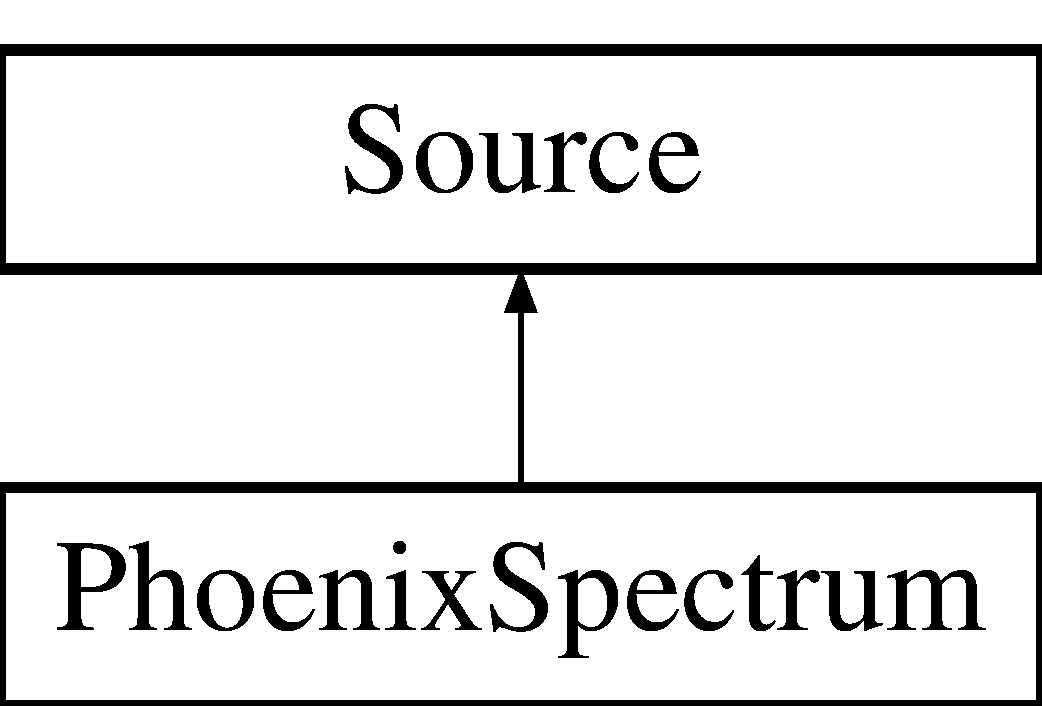
\includegraphics[height=2.000000cm]{class_phoenix_spectrum}
\end{center}
\end{figure}
\subsection*{Public Member Functions}
\begin{DoxyCompactItemize}
\item 
\hyperlink{class_phoenix_spectrum_a12bc8d55db0b852f04b03c4ea0f48884}{Phoenix\+Spectrum} (std\+::string spectrum\+\_\+file, std\+::string wavelength\+\_\+file, const double \&min\+\_\+wavelength, const double \&max\+\_\+wavelength)
\item 
void \hyperlink{class_phoenix_spectrum_a90e3cb19bdfaed4b5cd862bf00b64d2f}{read\+\_\+spectrum} (std\+::string spectrum\+\_\+file, std\+::string wavelength\+\_\+file, const double \&min\+\_\+wavelength, const double \&max\+\_\+wavelength)
\item 
double \hyperlink{class_phoenix_spectrum_a4e5ddcd25114f1a62a0f728165318fb1}{get\+\_\+spectral\+\_\+density} (double wavelength)
\end{DoxyCompactItemize}
\subsection*{Private Attributes}
\begin{DoxyCompactItemize}
\item 
std\+::map$<$ double, double $>$ \hyperlink{class_phoenix_spectrum_ac93c6be0579e2e0603dde85a24c189fe}{data}
\end{DoxyCompactItemize}


\subsection{Constructor \& Destructor Documentation}
\index{Phoenix\+Spectrum@{Phoenix\+Spectrum}!Phoenix\+Spectrum@{Phoenix\+Spectrum}}
\index{Phoenix\+Spectrum@{Phoenix\+Spectrum}!Phoenix\+Spectrum@{Phoenix\+Spectrum}}
\subsubsection[{\texorpdfstring{Phoenix\+Spectrum(std\+::string spectrum\+\_\+file, std\+::string wavelength\+\_\+file, const double \&min\+\_\+wavelength, const double \&max\+\_\+wavelength)}{PhoenixSpectrum(std::string spectrum_file, std::string wavelength_file, const double &min_wavelength, const double &max_wavelength)}}]{\setlength{\rightskip}{0pt plus 5cm}Phoenix\+Spectrum\+::\+Phoenix\+Spectrum (
\begin{DoxyParamCaption}
\item[{std\+::string}]{spectrum\+\_\+file, }
\item[{std\+::string}]{wavelength\+\_\+file, }
\item[{const double \&}]{min\+\_\+wavelength, }
\item[{const double \&}]{max\+\_\+wavelength}
\end{DoxyParamCaption}
)}\hypertarget{class_phoenix_spectrum_a12bc8d55db0b852f04b03c4ea0f48884}{}\label{class_phoenix_spectrum_a12bc8d55db0b852f04b03c4ea0f48884}


\subsection{Member Function Documentation}
\index{Phoenix\+Spectrum@{Phoenix\+Spectrum}!get\+\_\+spectral\+\_\+density@{get\+\_\+spectral\+\_\+density}}
\index{get\+\_\+spectral\+\_\+density@{get\+\_\+spectral\+\_\+density}!Phoenix\+Spectrum@{Phoenix\+Spectrum}}
\subsubsection[{\texorpdfstring{get\+\_\+spectral\+\_\+density(double wavelength)}{get_spectral_density(double wavelength)}}]{\setlength{\rightskip}{0pt plus 5cm}double Phoenix\+Spectrum\+::get\+\_\+spectral\+\_\+density (
\begin{DoxyParamCaption}
\item[{double}]{wavelength}
\end{DoxyParamCaption}
)\hspace{0.3cm}{\ttfamily [virtual]}}\hypertarget{class_phoenix_spectrum_a4e5ddcd25114f1a62a0f728165318fb1}{}\label{class_phoenix_spectrum_a4e5ddcd25114f1a62a0f728165318fb1}
This function returns the spectral density at a given wavelength. It is the essential function for all subclasses. \begin{DoxySeeAlso}{See also}
\hyperlink{class_source_ab5d90ab3a4cfb8403803d88ce8b9f0f8}{Source\+::get\+\_\+spectrum()} will use this function to integrate over it to retreive a spectrum for a given wavelength vector. 
\end{DoxySeeAlso}

\begin{DoxyParams}{Parameters}
{\em wavelength} & wavelength \\
\hline
\end{DoxyParams}
\begin{DoxyReturn}{Returns}
spectral density 
\end{DoxyReturn}


Reimplemented from \hyperlink{class_source_a546ae8ec1ae47e888c74f146278e19af}{Source}.

\index{Phoenix\+Spectrum@{Phoenix\+Spectrum}!read\+\_\+spectrum@{read\+\_\+spectrum}}
\index{read\+\_\+spectrum@{read\+\_\+spectrum}!Phoenix\+Spectrum@{Phoenix\+Spectrum}}
\subsubsection[{\texorpdfstring{read\+\_\+spectrum(std\+::string spectrum\+\_\+file, std\+::string wavelength\+\_\+file, const double \&min\+\_\+wavelength, const double \&max\+\_\+wavelength)}{read_spectrum(std::string spectrum_file, std::string wavelength_file, const double &min_wavelength, const double &max_wavelength)}}]{\setlength{\rightskip}{0pt plus 5cm}void Phoenix\+Spectrum\+::read\+\_\+spectrum (
\begin{DoxyParamCaption}
\item[{std\+::string}]{spectrum\+\_\+file, }
\item[{std\+::string}]{wavelength\+\_\+file, }
\item[{const double \&}]{min\+\_\+wavelength, }
\item[{const double \&}]{max\+\_\+wavelength}
\end{DoxyParamCaption}
)}\hypertarget{class_phoenix_spectrum_a90e3cb19bdfaed4b5cd862bf00b64d2f}{}\label{class_phoenix_spectrum_a90e3cb19bdfaed4b5cd862bf00b64d2f}


\subsection{Member Data Documentation}
\index{Phoenix\+Spectrum@{Phoenix\+Spectrum}!data@{data}}
\index{data@{data}!Phoenix\+Spectrum@{Phoenix\+Spectrum}}
\subsubsection[{\texorpdfstring{data}{data}}]{\setlength{\rightskip}{0pt plus 5cm}std\+::map$<$double, double$>$ Phoenix\+Spectrum\+::data\hspace{0.3cm}{\ttfamily [private]}}\hypertarget{class_phoenix_spectrum_ac93c6be0579e2e0603dde85a24c189fe}{}\label{class_phoenix_spectrum_ac93c6be0579e2e0603dde85a24c189fe}


The documentation for this class was generated from the following files\+:\begin{DoxyCompactItemize}
\item 
/home/stuermer/\+Repos/cpp/\+Echelle\+Simulator/include/\hyperlink{source_8h}{source.\+h}\item 
/home/stuermer/\+Repos/cpp/\+Echelle\+Simulator/src/\hyperlink{source_8cpp}{source.\+cpp}\end{DoxyCompactItemize}

\hypertarget{class_p_s_f}{}\section{P\+SF Class Reference}
\label{class_p_s_f}\index{P\+SF@{P\+SF}}


Class handles point spread functions.  




{\ttfamily \#include $<$P\+S\+F.\+h$>$}

Inheritance diagram for P\+SF\+:\begin{figure}[H]
\begin{center}
\leavevmode
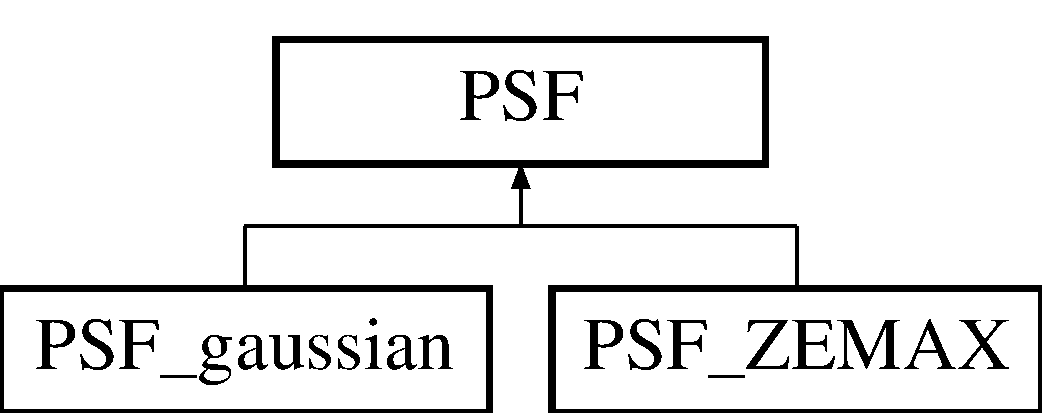
\includegraphics[height=2.000000cm]{class_p_s_f}
\end{center}
\end{figure}
\subsection*{Public Member Functions}
\begin{DoxyCompactItemize}
\item 
\hyperlink{class_p_s_f_ae71c0e4726ca7813fdcc3fe55b67d6d9}{P\+SF} ()
\item 
virtual \hyperlink{class_p_s_f_a3e8372a6dc5cc4a547ad6c92aa358807}{$\sim$\+P\+SF} ()
\item 
virtual cv\+::\+Mat \hyperlink{class_p_s_f_a136bdda01aeb3e8f2fc3554aa7d8be06}{get\+\_\+\+P\+SF} (int order, double wavelength)=0
\end{DoxyCompactItemize}


\subsection{Detailed Description}
Class handles point spread functions. 

This class handles point spread functions (P\+S\+Fs). It\textquotesingle{}s basic functionality is to deliver a \hyperlink{class_p_s_f}{P\+SF} as a 2d matrix for a given wavelength and order of an echelle spectrograph.

Typically the \hyperlink{class_p_s_f}{P\+SF} of an echelle spectrograph will vary across the \hyperlink{class_c_c_d}{C\+CD} depending on the wavelength, the echelle order, and the illumination of the optics. The \hyperlink{class_p_s_f}{P\+SF} might not be stable from target to target, as illumination might vary due to different coupling conditions and imperfect scrambling of the fibers.

To implement own \hyperlink{class_p_s_f}{P\+SF} classes, inherit from \hyperlink{class_p_s_f}{P\+SF} and overwrite get\+\_\+\+P\+SF function 

\subsection{Constructor \& Destructor Documentation}
\index{P\+SF@{P\+SF}!P\+SF@{P\+SF}}
\index{P\+SF@{P\+SF}!P\+SF@{P\+SF}}
\subsubsection[{\texorpdfstring{P\+S\+F()}{PSF()}}]{\setlength{\rightskip}{0pt plus 5cm}P\+S\+F\+::\+P\+SF (
\begin{DoxyParamCaption}
{}
\end{DoxyParamCaption}
)}\hypertarget{class_p_s_f_ae71c0e4726ca7813fdcc3fe55b67d6d9}{}\label{class_p_s_f_ae71c0e4726ca7813fdcc3fe55b67d6d9}
\index{P\+SF@{P\+SF}!````~P\+SF@{$\sim$\+P\+SF}}
\index{````~P\+SF@{$\sim$\+P\+SF}!P\+SF@{P\+SF}}
\subsubsection[{\texorpdfstring{$\sim$\+P\+S\+F()}{~PSF()}}]{\setlength{\rightskip}{0pt plus 5cm}P\+S\+F\+::$\sim$\+P\+SF (
\begin{DoxyParamCaption}
{}
\end{DoxyParamCaption}
)\hspace{0.3cm}{\ttfamily [virtual]}}\hypertarget{class_p_s_f_a3e8372a6dc5cc4a547ad6c92aa358807}{}\label{class_p_s_f_a3e8372a6dc5cc4a547ad6c92aa358807}


\subsection{Member Function Documentation}
\index{P\+SF@{P\+SF}!get\+\_\+\+P\+SF@{get\+\_\+\+P\+SF}}
\index{get\+\_\+\+P\+SF@{get\+\_\+\+P\+SF}!P\+SF@{P\+SF}}
\subsubsection[{\texorpdfstring{get\+\_\+\+P\+S\+F(int order, double wavelength)=0}{get_PSF(int order, double wavelength)=0}}]{\setlength{\rightskip}{0pt plus 5cm}virtual cv\+::\+Mat P\+S\+F\+::get\+\_\+\+P\+SF (
\begin{DoxyParamCaption}
\item[{int}]{order, }
\item[{double}]{wavelength}
\end{DoxyParamCaption}
)\hspace{0.3cm}{\ttfamily [pure virtual]}}\hypertarget{class_p_s_f_a136bdda01aeb3e8f2fc3554aa7d8be06}{}\label{class_p_s_f_a136bdda01aeb3e8f2fc3554aa7d8be06}


Implemented in \hyperlink{class_p_s_f__gaussian_a1f19bc740363485cd2e067f9580bafdd}{P\+S\+F\+\_\+gaussian}, and \hyperlink{class_p_s_f___z_e_m_a_x_a2fec338597b88e4f560489e9648649c5}{P\+S\+F\+\_\+\+Z\+E\+M\+AX}.



The documentation for this class was generated from the following files\+:\begin{DoxyCompactItemize}
\item 
/home/stuermer/\+Repos/cpp/\+Echelle\+Simulator/include/\hyperlink{_p_s_f_8h}{P\+S\+F.\+h}\item 
/home/stuermer/\+Repos/cpp/\+Echelle\+Simulator/src/\hyperlink{_p_s_f_8cpp}{P\+S\+F.\+cpp}\end{DoxyCompactItemize}

\hypertarget{class_p_s_f__gaussian}{}\section{P\+S\+F\+\_\+gaussian Class Reference}
\label{class_p_s_f__gaussian}\index{P\+S\+F\+\_\+gaussian@{P\+S\+F\+\_\+gaussian}}


{\ttfamily \#include $<$P\+S\+F.\+h$>$}

Inheritance diagram for P\+S\+F\+\_\+gaussian\+:\begin{figure}[H]
\begin{center}
\leavevmode
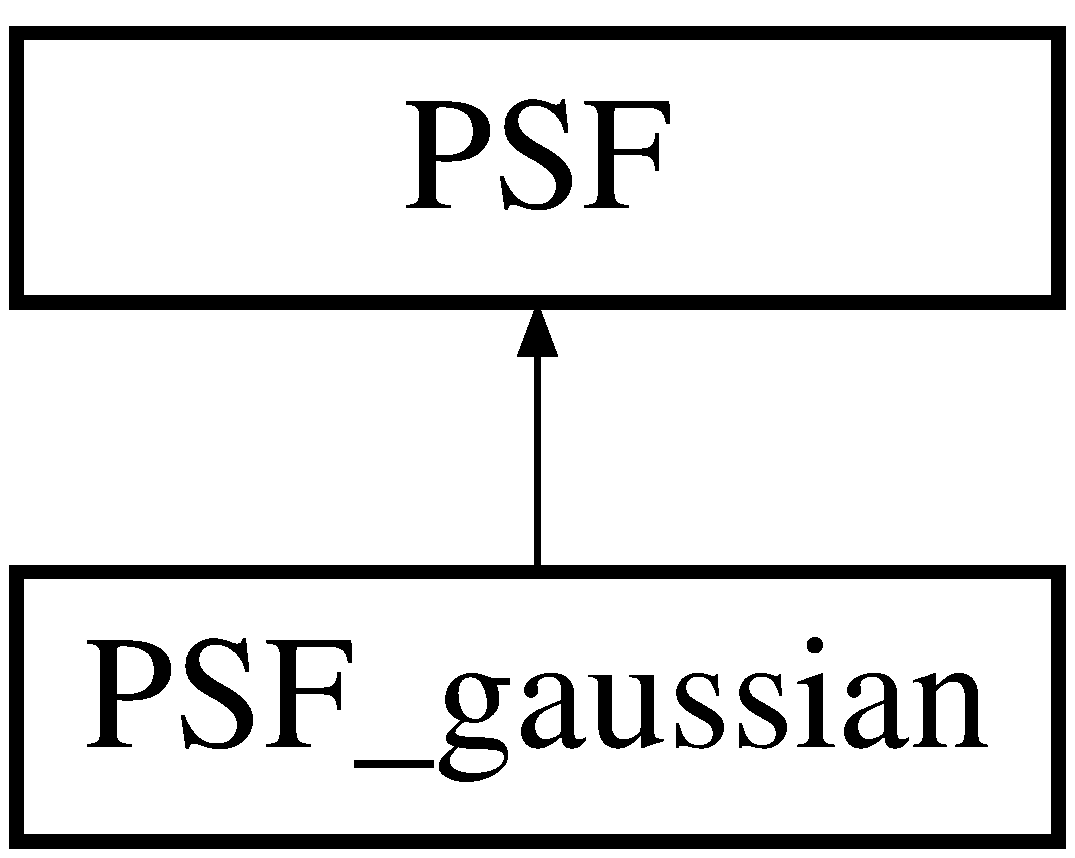
\includegraphics[height=2.000000cm]{class_p_s_f__gaussian}
\end{center}
\end{figure}
\subsection*{Public Member Functions}
\begin{DoxyCompactItemize}
\item 
\hyperlink{class_p_s_f__gaussian_a24935b42954caa3cb04b3926dc1f80e2}{P\+S\+F\+\_\+gaussian} (double \hyperlink{class_p_s_f__gaussian_ad0bcbd4165e73b7645f18906dd0d4aef}{sigma}, double aperture=3.)
\item 
cv\+::\+Mat \hyperlink{class_p_s_f__gaussian_a1f19bc740363485cd2e067f9580bafdd}{get\+\_\+\+P\+SF} (int order, double wavelength)
\end{DoxyCompactItemize}
\subsection*{Private Attributes}
\begin{DoxyCompactItemize}
\item 
double \hyperlink{class_p_s_f__gaussian_ad0bcbd4165e73b7645f18906dd0d4aef}{sigma}
\item 
int \hyperlink{class_p_s_f__gaussian_a553862ec78e59f6f36a67f9ddd50048c}{ksize}
\end{DoxyCompactItemize}


\subsection{Constructor \& Destructor Documentation}
\index{P\+S\+F\+\_\+gaussian@{P\+S\+F\+\_\+gaussian}!P\+S\+F\+\_\+gaussian@{P\+S\+F\+\_\+gaussian}}
\index{P\+S\+F\+\_\+gaussian@{P\+S\+F\+\_\+gaussian}!P\+S\+F\+\_\+gaussian@{P\+S\+F\+\_\+gaussian}}
\subsubsection[{\texorpdfstring{P\+S\+F\+\_\+gaussian(double sigma, double aperture=3.)}{PSF_gaussian(double sigma, double aperture=3.)}}]{\setlength{\rightskip}{0pt plus 5cm}P\+S\+F\+\_\+gaussian\+::\+P\+S\+F\+\_\+gaussian (
\begin{DoxyParamCaption}
\item[{double}]{sigma, }
\item[{double}]{aperture = {\ttfamily 3.}}
\end{DoxyParamCaption}
)}\hypertarget{class_p_s_f__gaussian_a24935b42954caa3cb04b3926dc1f80e2}{}\label{class_p_s_f__gaussian_a24935b42954caa3cb04b3926dc1f80e2}


\subsection{Member Function Documentation}
\index{P\+S\+F\+\_\+gaussian@{P\+S\+F\+\_\+gaussian}!get\+\_\+\+P\+SF@{get\+\_\+\+P\+SF}}
\index{get\+\_\+\+P\+SF@{get\+\_\+\+P\+SF}!P\+S\+F\+\_\+gaussian@{P\+S\+F\+\_\+gaussian}}
\subsubsection[{\texorpdfstring{get\+\_\+\+P\+S\+F(int order, double wavelength)}{get_PSF(int order, double wavelength)}}]{\setlength{\rightskip}{0pt plus 5cm}cv\+::\+Mat P\+S\+F\+\_\+gaussian\+::get\+\_\+\+P\+SF (
\begin{DoxyParamCaption}
\item[{int}]{order, }
\item[{double}]{wavelength}
\end{DoxyParamCaption}
)\hspace{0.3cm}{\ttfamily [virtual]}}\hypertarget{class_p_s_f__gaussian_a1f19bc740363485cd2e067f9580bafdd}{}\label{class_p_s_f__gaussian_a1f19bc740363485cd2e067f9580bafdd}


Implements \hyperlink{class_p_s_f_a136bdda01aeb3e8f2fc3554aa7d8be06}{P\+SF}.



\subsection{Member Data Documentation}
\index{P\+S\+F\+\_\+gaussian@{P\+S\+F\+\_\+gaussian}!ksize@{ksize}}
\index{ksize@{ksize}!P\+S\+F\+\_\+gaussian@{P\+S\+F\+\_\+gaussian}}
\subsubsection[{\texorpdfstring{ksize}{ksize}}]{\setlength{\rightskip}{0pt plus 5cm}int P\+S\+F\+\_\+gaussian\+::ksize\hspace{0.3cm}{\ttfamily [private]}}\hypertarget{class_p_s_f__gaussian_a553862ec78e59f6f36a67f9ddd50048c}{}\label{class_p_s_f__gaussian_a553862ec78e59f6f36a67f9ddd50048c}
\index{P\+S\+F\+\_\+gaussian@{P\+S\+F\+\_\+gaussian}!sigma@{sigma}}
\index{sigma@{sigma}!P\+S\+F\+\_\+gaussian@{P\+S\+F\+\_\+gaussian}}
\subsubsection[{\texorpdfstring{sigma}{sigma}}]{\setlength{\rightskip}{0pt plus 5cm}double P\+S\+F\+\_\+gaussian\+::sigma\hspace{0.3cm}{\ttfamily [private]}}\hypertarget{class_p_s_f__gaussian_ad0bcbd4165e73b7645f18906dd0d4aef}{}\label{class_p_s_f__gaussian_ad0bcbd4165e73b7645f18906dd0d4aef}


The documentation for this class was generated from the following files\+:\begin{DoxyCompactItemize}
\item 
/home/stuermer/\+Repos/cpp/\+Echelle\+Simulator/include/\hyperlink{_p_s_f_8h}{P\+S\+F.\+h}\item 
/home/stuermer/\+Repos/cpp/\+Echelle\+Simulator/src/\hyperlink{_p_s_f_8cpp}{P\+S\+F.\+cpp}\end{DoxyCompactItemize}

\hypertarget{class_p_s_f___z_e_m_a_x}{}\section{P\+S\+F\+\_\+\+Z\+E\+M\+AX Class Reference}
\label{class_p_s_f___z_e_m_a_x}\index{P\+S\+F\+\_\+\+Z\+E\+M\+AX@{P\+S\+F\+\_\+\+Z\+E\+M\+AX}}


{\ttfamily \#include $<$P\+S\+F.\+h$>$}

Inheritance diagram for P\+S\+F\+\_\+\+Z\+E\+M\+AX\+:\begin{figure}[H]
\begin{center}
\leavevmode
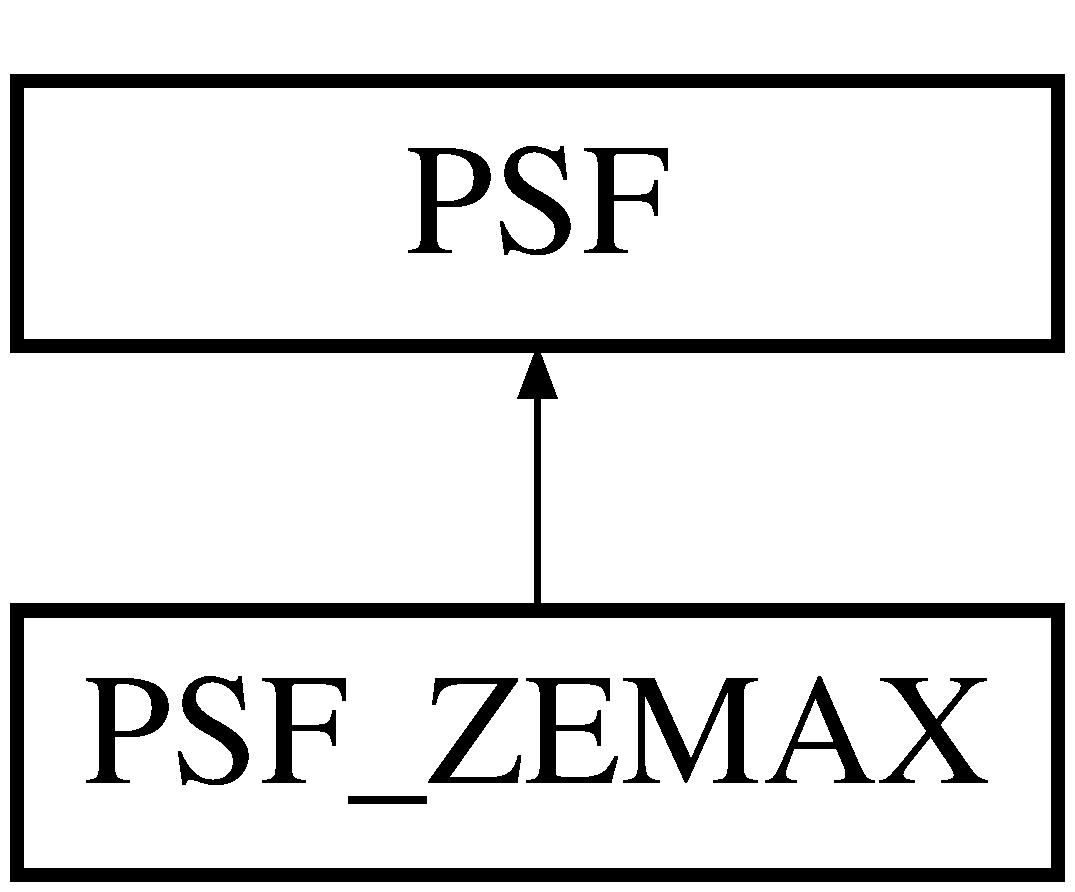
\includegraphics[height=2.000000cm]{class_p_s_f___z_e_m_a_x}
\end{center}
\end{figure}
\subsection*{Public Member Functions}
\begin{DoxyCompactItemize}
\item 
\hyperlink{class_p_s_f___z_e_m_a_x_aa1d613e53e5acb9744461efd35c2ef09}{P\+S\+F\+\_\+\+Z\+E\+M\+AX} (std\+::string filename, int fiber\+\_\+number)
\item 
cv\+::\+Mat \hyperlink{class_p_s_f___z_e_m_a_x_a2fec338597b88e4f560489e9648649c5}{get\+\_\+\+P\+SF} (int order, double wavelength)
\item 
cv\+::\+Mat \hyperlink{class_p_s_f___z_e_m_a_x_ad3b5bb955539e861246cc0f3e3add141}{interpolate\+\_\+\+P\+SF} (cv\+::\+Mat psf1, cv\+::\+Mat psf2, double w1, double w2, double w)
\end{DoxyCompactItemize}
\subsection*{Private Attributes}
\begin{DoxyCompactItemize}
\item 
std\+::map$<$ int, std\+::vector$<$ \hyperlink{struct_p_s_fdata}{P\+S\+Fdata} $>$ $>$ \hyperlink{class_p_s_f___z_e_m_a_x_af44c6c61ee1c43bfb34b98922f796bad}{psfs}
\end{DoxyCompactItemize}


\subsection{Constructor \& Destructor Documentation}
\index{P\+S\+F\+\_\+\+Z\+E\+M\+AX@{P\+S\+F\+\_\+\+Z\+E\+M\+AX}!P\+S\+F\+\_\+\+Z\+E\+M\+AX@{P\+S\+F\+\_\+\+Z\+E\+M\+AX}}
\index{P\+S\+F\+\_\+\+Z\+E\+M\+AX@{P\+S\+F\+\_\+\+Z\+E\+M\+AX}!P\+S\+F\+\_\+\+Z\+E\+M\+AX@{P\+S\+F\+\_\+\+Z\+E\+M\+AX}}
\subsubsection[{\texorpdfstring{P\+S\+F\+\_\+\+Z\+E\+M\+A\+X(std\+::string filename, int fiber\+\_\+number)}{PSF_ZEMAX(std::string filename, int fiber_number)}}]{\setlength{\rightskip}{0pt plus 5cm}P\+S\+F\+\_\+\+Z\+E\+M\+A\+X\+::\+P\+S\+F\+\_\+\+Z\+E\+M\+AX (
\begin{DoxyParamCaption}
\item[{std\+::string}]{filename, }
\item[{int}]{fiber\+\_\+number}
\end{DoxyParamCaption}
)}\hypertarget{class_p_s_f___z_e_m_a_x_aa1d613e53e5acb9744461efd35c2ef09}{}\label{class_p_s_f___z_e_m_a_x_aa1d613e53e5acb9744461efd35c2ef09}


\subsection{Member Function Documentation}
\index{P\+S\+F\+\_\+\+Z\+E\+M\+AX@{P\+S\+F\+\_\+\+Z\+E\+M\+AX}!get\+\_\+\+P\+SF@{get\+\_\+\+P\+SF}}
\index{get\+\_\+\+P\+SF@{get\+\_\+\+P\+SF}!P\+S\+F\+\_\+\+Z\+E\+M\+AX@{P\+S\+F\+\_\+\+Z\+E\+M\+AX}}
\subsubsection[{\texorpdfstring{get\+\_\+\+P\+S\+F(int order, double wavelength)}{get_PSF(int order, double wavelength)}}]{\setlength{\rightskip}{0pt plus 5cm}cv\+::\+Mat P\+S\+F\+\_\+\+Z\+E\+M\+A\+X\+::get\+\_\+\+P\+SF (
\begin{DoxyParamCaption}
\item[{int}]{order, }
\item[{double}]{wavelength}
\end{DoxyParamCaption}
)\hspace{0.3cm}{\ttfamily [virtual]}}\hypertarget{class_p_s_f___z_e_m_a_x_a2fec338597b88e4f560489e9648649c5}{}\label{class_p_s_f___z_e_m_a_x_a2fec338597b88e4f560489e9648649c5}


Implements \hyperlink{class_p_s_f_a136bdda01aeb3e8f2fc3554aa7d8be06}{P\+SF}.

\index{P\+S\+F\+\_\+\+Z\+E\+M\+AX@{P\+S\+F\+\_\+\+Z\+E\+M\+AX}!interpolate\+\_\+\+P\+SF@{interpolate\+\_\+\+P\+SF}}
\index{interpolate\+\_\+\+P\+SF@{interpolate\+\_\+\+P\+SF}!P\+S\+F\+\_\+\+Z\+E\+M\+AX@{P\+S\+F\+\_\+\+Z\+E\+M\+AX}}
\subsubsection[{\texorpdfstring{interpolate\+\_\+\+P\+S\+F(cv\+::\+Mat psf1, cv\+::\+Mat psf2, double w1, double w2, double w)}{interpolate_PSF(cv::Mat psf1, cv::Mat psf2, double w1, double w2, double w)}}]{\setlength{\rightskip}{0pt plus 5cm}cv\+::\+Mat P\+S\+F\+\_\+\+Z\+E\+M\+A\+X\+::interpolate\+\_\+\+P\+SF (
\begin{DoxyParamCaption}
\item[{cv\+::\+Mat}]{psf1, }
\item[{cv\+::\+Mat}]{psf2, }
\item[{double}]{w1, }
\item[{double}]{w2, }
\item[{double}]{w}
\end{DoxyParamCaption}
)}\hypertarget{class_p_s_f___z_e_m_a_x_ad3b5bb955539e861246cc0f3e3add141}{}\label{class_p_s_f___z_e_m_a_x_ad3b5bb955539e861246cc0f3e3add141}


\subsection{Member Data Documentation}
\index{P\+S\+F\+\_\+\+Z\+E\+M\+AX@{P\+S\+F\+\_\+\+Z\+E\+M\+AX}!psfs@{psfs}}
\index{psfs@{psfs}!P\+S\+F\+\_\+\+Z\+E\+M\+AX@{P\+S\+F\+\_\+\+Z\+E\+M\+AX}}
\subsubsection[{\texorpdfstring{psfs}{psfs}}]{\setlength{\rightskip}{0pt plus 5cm}std\+::map$<$ int, std\+::vector$<${\bf P\+S\+Fdata}$>$ $>$ P\+S\+F\+\_\+\+Z\+E\+M\+A\+X\+::psfs\hspace{0.3cm}{\ttfamily [private]}}\hypertarget{class_p_s_f___z_e_m_a_x_af44c6c61ee1c43bfb34b98922f796bad}{}\label{class_p_s_f___z_e_m_a_x_af44c6c61ee1c43bfb34b98922f796bad}


The documentation for this class was generated from the following files\+:\begin{DoxyCompactItemize}
\item 
/home/stuermer/\+Repos/cpp/\+Echelle\+Simulator/include/\hyperlink{_p_s_f_8h}{P\+S\+F.\+h}\item 
/home/stuermer/\+Repos/cpp/\+Echelle\+Simulator/src/\hyperlink{_p_s_f_8cpp}{P\+S\+F.\+cpp}\end{DoxyCompactItemize}

\hypertarget{struct_p_s_fdata}{}\section{P\+S\+Fdata Struct Reference}
\label{struct_p_s_fdata}\index{P\+S\+Fdata@{P\+S\+Fdata}}


{\ttfamily \#include $<$P\+S\+F.\+h$>$}

\subsection*{Public Member Functions}
\begin{DoxyCompactItemize}
\item 
\hyperlink{struct_p_s_fdata_a716864fd12b8169ed6253757dffbee9e}{P\+S\+Fdata} (double w, cv\+::\+Mat p)
\item 
bool \hyperlink{struct_p_s_fdata_a7ca41b4250b8a9dda6f141fe426b9e02}{operator$<$} (const \hyperlink{struct_p_s_fdata}{P\+S\+Fdata} \&str) const 
\end{DoxyCompactItemize}
\subsection*{Public Attributes}
\begin{DoxyCompactItemize}
\item 
double \hyperlink{struct_p_s_fdata_acad9e0c352a0a7bada4b8ac89ff5487e}{wavelength}
\item 
cv\+::\+Mat \hyperlink{struct_p_s_fdata_a4947cba76060627e31534f978fd83804}{psf}
\end{DoxyCompactItemize}


\subsection{Constructor \& Destructor Documentation}
\index{P\+S\+Fdata@{P\+S\+Fdata}!P\+S\+Fdata@{P\+S\+Fdata}}
\index{P\+S\+Fdata@{P\+S\+Fdata}!P\+S\+Fdata@{P\+S\+Fdata}}
\subsubsection[{\texorpdfstring{P\+S\+Fdata(double w, cv\+::\+Mat p)}{PSFdata(double w, cv::Mat p)}}]{\setlength{\rightskip}{0pt plus 5cm}P\+S\+Fdata\+::\+P\+S\+Fdata (
\begin{DoxyParamCaption}
\item[{double}]{w, }
\item[{cv\+::\+Mat}]{p}
\end{DoxyParamCaption}
)\hspace{0.3cm}{\ttfamily [inline]}}\hypertarget{struct_p_s_fdata_a716864fd12b8169ed6253757dffbee9e}{}\label{struct_p_s_fdata_a716864fd12b8169ed6253757dffbee9e}


\subsection{Member Function Documentation}
\index{P\+S\+Fdata@{P\+S\+Fdata}!operator$<$@{operator$<$}}
\index{operator$<$@{operator$<$}!P\+S\+Fdata@{P\+S\+Fdata}}
\subsubsection[{\texorpdfstring{operator$<$(const P\+S\+Fdata \&str) const }{operator<(const PSFdata &str) const }}]{\setlength{\rightskip}{0pt plus 5cm}bool P\+S\+Fdata\+::operator$<$ (
\begin{DoxyParamCaption}
\item[{const {\bf P\+S\+Fdata} \&}]{str}
\end{DoxyParamCaption}
) const\hspace{0.3cm}{\ttfamily [inline]}}\hypertarget{struct_p_s_fdata_a7ca41b4250b8a9dda6f141fe426b9e02}{}\label{struct_p_s_fdata_a7ca41b4250b8a9dda6f141fe426b9e02}


\subsection{Member Data Documentation}
\index{P\+S\+Fdata@{P\+S\+Fdata}!psf@{psf}}
\index{psf@{psf}!P\+S\+Fdata@{P\+S\+Fdata}}
\subsubsection[{\texorpdfstring{psf}{psf}}]{\setlength{\rightskip}{0pt plus 5cm}cv\+::\+Mat P\+S\+Fdata\+::psf}\hypertarget{struct_p_s_fdata_a4947cba76060627e31534f978fd83804}{}\label{struct_p_s_fdata_a4947cba76060627e31534f978fd83804}
\index{P\+S\+Fdata@{P\+S\+Fdata}!wavelength@{wavelength}}
\index{wavelength@{wavelength}!P\+S\+Fdata@{P\+S\+Fdata}}
\subsubsection[{\texorpdfstring{wavelength}{wavelength}}]{\setlength{\rightskip}{0pt plus 5cm}double P\+S\+Fdata\+::wavelength}\hypertarget{struct_p_s_fdata_acad9e0c352a0a7bada4b8ac89ff5487e}{}\label{struct_p_s_fdata_acad9e0c352a0a7bada4b8ac89ff5487e}


The documentation for this struct was generated from the following file\+:\begin{DoxyCompactItemize}
\item 
/home/stuermer/\+Repos/cpp/\+Echelle\+Simulator/include/\hyperlink{_p_s_f_8h}{P\+S\+F.\+h}\end{DoxyCompactItemize}

\hypertarget{structraw__transformation}{}\section{raw\+\_\+transformation Struct Reference}
\label{structraw__transformation}\index{raw\+\_\+transformation@{raw\+\_\+transformation}}


{\ttfamily \#include $<$matrixsimulator.\+h$>$}

\subsection*{Public Attributes}
\begin{DoxyCompactItemize}
\item 
int \hyperlink{structraw__transformation_a896cd09845802341d970910f7b6a1617}{order}
\item 
double \hyperlink{structraw__transformation_a8cfb4c9736421e670f53d8eebb4d82ef}{wavelength}
\item 
cv\+::\+Mat \hyperlink{structraw__transformation_a664c5ba015a8d2c1cbd10a3787a306f3}{transformation\+\_\+matrix} = cv\+::\+Mat(2,3,C\+V\+\_\+64\+F\+C1)
\item 
std\+::vector$<$ double $>$ \hyperlink{structraw__transformation_ae5c78a8434f7ce62f1f147cf4574dde7}{decomposed\+\_\+matrix}
\end{DoxyCompactItemize}


\subsection{Member Data Documentation}
\index{raw\+\_\+transformation@{raw\+\_\+transformation}!decomposed\+\_\+matrix@{decomposed\+\_\+matrix}}
\index{decomposed\+\_\+matrix@{decomposed\+\_\+matrix}!raw\+\_\+transformation@{raw\+\_\+transformation}}
\subsubsection[{\texorpdfstring{decomposed\+\_\+matrix}{decomposed_matrix}}]{\setlength{\rightskip}{0pt plus 5cm}std\+::vector$<$double$>$ raw\+\_\+transformation\+::decomposed\+\_\+matrix}\hypertarget{structraw__transformation_ae5c78a8434f7ce62f1f147cf4574dde7}{}\label{structraw__transformation_ae5c78a8434f7ce62f1f147cf4574dde7}
\index{raw\+\_\+transformation@{raw\+\_\+transformation}!order@{order}}
\index{order@{order}!raw\+\_\+transformation@{raw\+\_\+transformation}}
\subsubsection[{\texorpdfstring{order}{order}}]{\setlength{\rightskip}{0pt plus 5cm}int raw\+\_\+transformation\+::order}\hypertarget{structraw__transformation_a896cd09845802341d970910f7b6a1617}{}\label{structraw__transformation_a896cd09845802341d970910f7b6a1617}
\index{raw\+\_\+transformation@{raw\+\_\+transformation}!transformation\+\_\+matrix@{transformation\+\_\+matrix}}
\index{transformation\+\_\+matrix@{transformation\+\_\+matrix}!raw\+\_\+transformation@{raw\+\_\+transformation}}
\subsubsection[{\texorpdfstring{transformation\+\_\+matrix}{transformation_matrix}}]{\setlength{\rightskip}{0pt plus 5cm}cv\+::\+Mat raw\+\_\+transformation\+::transformation\+\_\+matrix = cv\+::\+Mat(2,3,C\+V\+\_\+64\+F\+C1)}\hypertarget{structraw__transformation_a664c5ba015a8d2c1cbd10a3787a306f3}{}\label{structraw__transformation_a664c5ba015a8d2c1cbd10a3787a306f3}
\index{raw\+\_\+transformation@{raw\+\_\+transformation}!wavelength@{wavelength}}
\index{wavelength@{wavelength}!raw\+\_\+transformation@{raw\+\_\+transformation}}
\subsubsection[{\texorpdfstring{wavelength}{wavelength}}]{\setlength{\rightskip}{0pt plus 5cm}double raw\+\_\+transformation\+::wavelength}\hypertarget{structraw__transformation_a8cfb4c9736421e670f53d8eebb4d82ef}{}\label{structraw__transformation_a8cfb4c9736421e670f53d8eebb4d82ef}


The documentation for this struct was generated from the following file\+:\begin{DoxyCompactItemize}
\item 
/home/stuermer/\+Repos/cpp/\+Echelle\+Simulator/include/\hyperlink{matrixsimulator_8h}{matrixsimulator.\+h}\end{DoxyCompactItemize}

\hypertarget{class_slit}{}\section{Slit Class Reference}
\label{class_slit}\index{Slit@{Slit}}


{\ttfamily \#include $<$Slit.\+h$>$}

\subsection*{Public Member Functions}
\begin{DoxyCompactItemize}
\item 
\hyperlink{class_slit_a64e4cabe34422a95f11ecc0069347b16}{Slit} ()
\item 
\hyperlink{class_slit_ace3c25bd92a26fc1e90e7e97525f3c90}{Slit} (double \hyperlink{class_slit_ae33a1c4c7205343947d2d3efdfdbd1dc}{w}, double \hyperlink{class_slit_a01efae646d51d27448701f31bd0d93dd}{h}, int \hyperlink{class_slit_ad5af377fe458ceb5c391be67ee58ac7b}{slit\+\_\+sampling})
\item 
void \hyperlink{class_slit_ad284e68cbdc279e58a6fd15dae919b90}{set\+\_\+slit} (double \hyperlink{class_slit_ae33a1c4c7205343947d2d3efdfdbd1dc}{w}, double \hyperlink{class_slit_a01efae646d51d27448701f31bd0d93dd}{h}, int \hyperlink{class_slit_ad5af377fe458ceb5c391be67ee58ac7b}{slit\+\_\+sampling})
\item 
void \hyperlink{class_slit_aea877be5c12b83fe5a50ee95ac2935db}{show} ()
\end{DoxyCompactItemize}
\subsection*{Public Attributes}
\begin{DoxyCompactItemize}
\item 
double \hyperlink{class_slit_ae33a1c4c7205343947d2d3efdfdbd1dc}{w}
\item 
double \hyperlink{class_slit_a01efae646d51d27448701f31bd0d93dd}{h}
\item 
int \hyperlink{class_slit_ae6998ed65fc4b82946152b723786fc6c}{w\+\_\+px}
\item 
int \hyperlink{class_slit_a1111ee8f26d476bcf047225ed8cd30e5}{h\+\_\+px}
\item 
double \hyperlink{class_slit_a28fd1dfc764c0cb46b40c5370708e4ff}{ratio}
\item 
int \hyperlink{class_slit_ad5af377fe458ceb5c391be67ee58ac7b}{slit\+\_\+sampling}
\item 
cv\+::\+Mat \hyperlink{class_slit_a3413479f87256e54dbd0a517b36f26e9}{slit\+\_\+image}
\item 
bool \hyperlink{class_slit_af27ddf455c96b348f6b0f5c221e41b20}{use\+\_\+gpu} = false
\end{DoxyCompactItemize}


\subsection{Constructor \& Destructor Documentation}
\index{Slit@{Slit}!Slit@{Slit}}
\index{Slit@{Slit}!Slit@{Slit}}
\subsubsection[{\texorpdfstring{Slit()}{Slit()}}]{\setlength{\rightskip}{0pt plus 5cm}Slit\+::\+Slit (
\begin{DoxyParamCaption}
{}
\end{DoxyParamCaption}
)}\hypertarget{class_slit_a64e4cabe34422a95f11ecc0069347b16}{}\label{class_slit_a64e4cabe34422a95f11ecc0069347b16}
\index{Slit@{Slit}!Slit@{Slit}}
\index{Slit@{Slit}!Slit@{Slit}}
\subsubsection[{\texorpdfstring{Slit(double w, double h, int slit\+\_\+sampling)}{Slit(double w, double h, int slit_sampling)}}]{\setlength{\rightskip}{0pt plus 5cm}Slit\+::\+Slit (
\begin{DoxyParamCaption}
\item[{double}]{w, }
\item[{double}]{h, }
\item[{int}]{slit\+\_\+sampling}
\end{DoxyParamCaption}
)}\hypertarget{class_slit_ace3c25bd92a26fc1e90e7e97525f3c90}{}\label{class_slit_ace3c25bd92a26fc1e90e7e97525f3c90}


\subsection{Member Function Documentation}
\index{Slit@{Slit}!set\+\_\+slit@{set\+\_\+slit}}
\index{set\+\_\+slit@{set\+\_\+slit}!Slit@{Slit}}
\subsubsection[{\texorpdfstring{set\+\_\+slit(double w, double h, int slit\+\_\+sampling)}{set_slit(double w, double h, int slit_sampling)}}]{\setlength{\rightskip}{0pt plus 5cm}void Slit\+::set\+\_\+slit (
\begin{DoxyParamCaption}
\item[{double}]{w, }
\item[{double}]{h, }
\item[{int}]{slit\+\_\+sampling}
\end{DoxyParamCaption}
)}\hypertarget{class_slit_ad284e68cbdc279e58a6fd15dae919b90}{}\label{class_slit_ad284e68cbdc279e58a6fd15dae919b90}
\index{Slit@{Slit}!show@{show}}
\index{show@{show}!Slit@{Slit}}
\subsubsection[{\texorpdfstring{show()}{show()}}]{\setlength{\rightskip}{0pt plus 5cm}void Slit\+::show (
\begin{DoxyParamCaption}
{}
\end{DoxyParamCaption}
)}\hypertarget{class_slit_aea877be5c12b83fe5a50ee95ac2935db}{}\label{class_slit_aea877be5c12b83fe5a50ee95ac2935db}


\subsection{Member Data Documentation}
\index{Slit@{Slit}!h@{h}}
\index{h@{h}!Slit@{Slit}}
\subsubsection[{\texorpdfstring{h}{h}}]{\setlength{\rightskip}{0pt plus 5cm}double Slit\+::h}\hypertarget{class_slit_a01efae646d51d27448701f31bd0d93dd}{}\label{class_slit_a01efae646d51d27448701f31bd0d93dd}
\index{Slit@{Slit}!h\+\_\+px@{h\+\_\+px}}
\index{h\+\_\+px@{h\+\_\+px}!Slit@{Slit}}
\subsubsection[{\texorpdfstring{h\+\_\+px}{h_px}}]{\setlength{\rightskip}{0pt plus 5cm}int Slit\+::h\+\_\+px}\hypertarget{class_slit_a1111ee8f26d476bcf047225ed8cd30e5}{}\label{class_slit_a1111ee8f26d476bcf047225ed8cd30e5}
\index{Slit@{Slit}!ratio@{ratio}}
\index{ratio@{ratio}!Slit@{Slit}}
\subsubsection[{\texorpdfstring{ratio}{ratio}}]{\setlength{\rightskip}{0pt plus 5cm}double Slit\+::ratio}\hypertarget{class_slit_a28fd1dfc764c0cb46b40c5370708e4ff}{}\label{class_slit_a28fd1dfc764c0cb46b40c5370708e4ff}
\index{Slit@{Slit}!slit\+\_\+image@{slit\+\_\+image}}
\index{slit\+\_\+image@{slit\+\_\+image}!Slit@{Slit}}
\subsubsection[{\texorpdfstring{slit\+\_\+image}{slit_image}}]{\setlength{\rightskip}{0pt plus 5cm}cv\+::\+Mat Slit\+::slit\+\_\+image}\hypertarget{class_slit_a3413479f87256e54dbd0a517b36f26e9}{}\label{class_slit_a3413479f87256e54dbd0a517b36f26e9}
\index{Slit@{Slit}!slit\+\_\+sampling@{slit\+\_\+sampling}}
\index{slit\+\_\+sampling@{slit\+\_\+sampling}!Slit@{Slit}}
\subsubsection[{\texorpdfstring{slit\+\_\+sampling}{slit_sampling}}]{\setlength{\rightskip}{0pt plus 5cm}int Slit\+::slit\+\_\+sampling}\hypertarget{class_slit_ad5af377fe458ceb5c391be67ee58ac7b}{}\label{class_slit_ad5af377fe458ceb5c391be67ee58ac7b}
\index{Slit@{Slit}!use\+\_\+gpu@{use\+\_\+gpu}}
\index{use\+\_\+gpu@{use\+\_\+gpu}!Slit@{Slit}}
\subsubsection[{\texorpdfstring{use\+\_\+gpu}{use_gpu}}]{\setlength{\rightskip}{0pt plus 5cm}bool Slit\+::use\+\_\+gpu = false}\hypertarget{class_slit_af27ddf455c96b348f6b0f5c221e41b20}{}\label{class_slit_af27ddf455c96b348f6b0f5c221e41b20}
\index{Slit@{Slit}!w@{w}}
\index{w@{w}!Slit@{Slit}}
\subsubsection[{\texorpdfstring{w}{w}}]{\setlength{\rightskip}{0pt plus 5cm}double Slit\+::w}\hypertarget{class_slit_ae33a1c4c7205343947d2d3efdfdbd1dc}{}\label{class_slit_ae33a1c4c7205343947d2d3efdfdbd1dc}
\index{Slit@{Slit}!w\+\_\+px@{w\+\_\+px}}
\index{w\+\_\+px@{w\+\_\+px}!Slit@{Slit}}
\subsubsection[{\texorpdfstring{w\+\_\+px}{w_px}}]{\setlength{\rightskip}{0pt plus 5cm}int Slit\+::w\+\_\+px}\hypertarget{class_slit_ae6998ed65fc4b82946152b723786fc6c}{}\label{class_slit_ae6998ed65fc4b82946152b723786fc6c}


The documentation for this class was generated from the following files\+:\begin{DoxyCompactItemize}
\item 
/home/stuermer/\+Repos/cpp/\+Echelle\+Simulator/include/\hyperlink{_slit_8h}{Slit.\+h}\item 
/home/stuermer/\+Repos/cpp/\+Echelle\+Simulator/src/\hyperlink{_slit_8cpp}{Slit.\+cpp}\end{DoxyCompactItemize}

\hypertarget{class_source}{}\section{Source Class Reference}
\label{class_source}\index{Source@{Source}}


Base class of all spectral sources.  




{\ttfamily \#include $<$source.\+h$>$}

Inheritance diagram for Source\+:\begin{figure}[H]
\begin{center}
\leavevmode
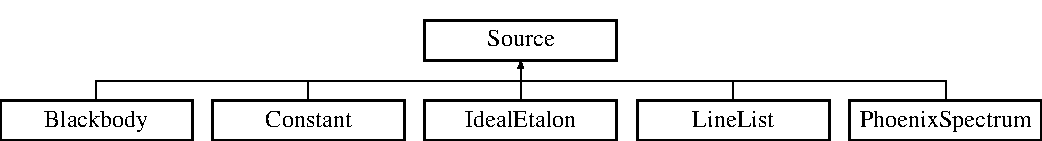
\includegraphics[height=1.898305cm]{class_source}
\end{center}
\end{figure}
\subsection*{Public Member Functions}
\begin{DoxyCompactItemize}
\item 
\hyperlink{class_source_a660c0a4b8b8f8402568bef86f2cb2fbb}{Source} ()
\item 
virtual \hyperlink{class_source_ac5104a4d66641ae529419b47da4a1473}{$\sim$\+Source} ()
\item 
virtual std\+::vector$<$ double $>$ \hyperlink{class_source_a165b9f7281915b5fdf5ce3278fb1e3aa}{get\+\_\+spectral\+\_\+density} (std\+::vector$<$ double $>$ wavelength)
\item 
virtual double \hyperlink{class_source_a546ae8ec1ae47e888c74f146278e19af}{get\+\_\+spectral\+\_\+density} (double wavelength)
\item 
virtual std\+::vector$<$ double $>$ \hyperlink{class_source_ab5d90ab3a4cfb8403803d88ce8b9f0f8}{get\+\_\+spectrum} (std\+::vector$<$ double $>$ wavelength)
\item 
void \hyperlink{class_source_a0bd707ab373bc9b957cb30d577af8a07}{set\+\_\+doppler\+\_\+shift} (double \hyperlink{class_source_a33104a788577b65918c95d240110c082}{shift})
\item 
void \hyperlink{class_source_a5d2eac20504111cbee890666e052e4df}{set\+\_\+integration\+\_\+steps} (int n)
\end{DoxyCompactItemize}
\subsection*{Private Member Functions}
\begin{DoxyCompactItemize}
\item 
double \hyperlink{class_source_ade0a7e2d3911f3247748ac21ab15e585}{integral\+\_\+s} (double a, double b, int n)
\end{DoxyCompactItemize}
\subsection*{Private Attributes}
\begin{DoxyCompactItemize}
\item 
double \hyperlink{class_source_a33104a788577b65918c95d240110c082}{shift}
\begin{DoxyCompactList}\small\item\em current doppler shift \end{DoxyCompactList}\item 
int \hyperlink{class_source_ac2c09694b86c1936b386afac137126e5}{integration\+\_\+steps}
\begin{DoxyCompactList}\small\item\em number of steps for the integrator \end{DoxyCompactList}\end{DoxyCompactItemize}


\subsection{Detailed Description}
Base class of all spectral sources. 

This class is the base class of all spectral sources. Its purpose is to provide a common interface for all sources. For implementing a new spectral source, inherit from this class and implement the \hyperlink{class_source_a165b9f7281915b5fdf5ce3278fb1e3aa}{Source\+::get\+\_\+spectral\+\_\+density} function. 

\subsection{Constructor \& Destructor Documentation}
\index{Source@{Source}!Source@{Source}}
\index{Source@{Source}!Source@{Source}}
\subsubsection[{\texorpdfstring{Source()}{Source()}}]{\setlength{\rightskip}{0pt plus 5cm}Source\+::\+Source (
\begin{DoxyParamCaption}
{}
\end{DoxyParamCaption}
)}\hypertarget{class_source_a660c0a4b8b8f8402568bef86f2cb2fbb}{}\label{class_source_a660c0a4b8b8f8402568bef86f2cb2fbb}
\index{Source@{Source}!````~Source@{$\sim$\+Source}}
\index{````~Source@{$\sim$\+Source}!Source@{Source}}
\subsubsection[{\texorpdfstring{$\sim$\+Source()}{~Source()}}]{\setlength{\rightskip}{0pt plus 5cm}Source\+::$\sim$\+Source (
\begin{DoxyParamCaption}
{}
\end{DoxyParamCaption}
)\hspace{0.3cm}{\ttfamily [virtual]}}\hypertarget{class_source_ac5104a4d66641ae529419b47da4a1473}{}\label{class_source_ac5104a4d66641ae529419b47da4a1473}


\subsection{Member Function Documentation}
\index{Source@{Source}!get\+\_\+spectral\+\_\+density@{get\+\_\+spectral\+\_\+density}}
\index{get\+\_\+spectral\+\_\+density@{get\+\_\+spectral\+\_\+density}!Source@{Source}}
\subsubsection[{\texorpdfstring{get\+\_\+spectral\+\_\+density(std\+::vector$<$ double $>$ wavelength)}{get_spectral_density(std::vector< double > wavelength)}}]{\setlength{\rightskip}{0pt plus 5cm}std\+::vector$<$ double $>$ Source\+::get\+\_\+spectral\+\_\+density (
\begin{DoxyParamCaption}
\item[{std\+::vector$<$ double $>$}]{wavelength}
\end{DoxyParamCaption}
)\hspace{0.3cm}{\ttfamily [virtual]}}\hypertarget{class_source_a165b9f7281915b5fdf5ce3278fb1e3aa}{}\label{class_source_a165b9f7281915b5fdf5ce3278fb1e3aa}
This is an overloaded member function, provided for convenience. It differs from the above function only in what argument(s) it accepts.

Returns the spectral density of the \hyperlink{class_source}{Source} at the given wavelength vector.


\begin{DoxyParams}{Parameters}
{\em wavelength} & wavelength vector \\
\hline
\end{DoxyParams}
\begin{DoxyReturn}{Returns}
spectral density at given wavelength 
\end{DoxyReturn}
\index{Source@{Source}!get\+\_\+spectral\+\_\+density@{get\+\_\+spectral\+\_\+density}}
\index{get\+\_\+spectral\+\_\+density@{get\+\_\+spectral\+\_\+density}!Source@{Source}}
\subsubsection[{\texorpdfstring{get\+\_\+spectral\+\_\+density(double wavelength)}{get_spectral_density(double wavelength)}}]{\setlength{\rightskip}{0pt plus 5cm}double Source\+::get\+\_\+spectral\+\_\+density (
\begin{DoxyParamCaption}
\item[{double}]{wavelength}
\end{DoxyParamCaption}
)\hspace{0.3cm}{\ttfamily [virtual]}}\hypertarget{class_source_a546ae8ec1ae47e888c74f146278e19af}{}\label{class_source_a546ae8ec1ae47e888c74f146278e19af}
This function returns the spectral density at a given wavelength. It is the essential function for all subclasses. \begin{DoxySeeAlso}{See also}
\hyperlink{class_source_ab5d90ab3a4cfb8403803d88ce8b9f0f8}{Source\+::get\+\_\+spectrum()} will use this function to integrate over it to retreive a spectrum for a given wavelength vector. 
\end{DoxySeeAlso}

\begin{DoxyParams}{Parameters}
{\em wavelength} & wavelength \\
\hline
\end{DoxyParams}
\begin{DoxyReturn}{Returns}
spectral density 
\end{DoxyReturn}


Reimplemented in \hyperlink{class_line_list_acb1e41d6120cf6bc0df2afaeb35a5aad}{Line\+List}, \hyperlink{class_phoenix_spectrum_a4e5ddcd25114f1a62a0f728165318fb1}{Phoenix\+Spectrum}, \hyperlink{class_blackbody_a2e667cd4c4362550a77eb9081258ffb3}{Blackbody}, \hyperlink{class_ideal_etalon_a6ba6c6d89e88e646da38ec45d12dab09}{Ideal\+Etalon}, and \hyperlink{class_constant_ae0526443e519154bcd338ee930bcad04}{Constant}.

\index{Source@{Source}!get\+\_\+spectrum@{get\+\_\+spectrum}}
\index{get\+\_\+spectrum@{get\+\_\+spectrum}!Source@{Source}}
\subsubsection[{\texorpdfstring{get\+\_\+spectrum(std\+::vector$<$ double $>$ wavelength)}{get_spectrum(std::vector< double > wavelength)}}]{\setlength{\rightskip}{0pt plus 5cm}std\+::vector$<$ double $>$ Source\+::get\+\_\+spectrum (
\begin{DoxyParamCaption}
\item[{std\+::vector$<$ double $>$}]{wavelength}
\end{DoxyParamCaption}
)\hspace{0.3cm}{\ttfamily [virtual]}}\hypertarget{class_source_ab5d90ab3a4cfb8403803d88ce8b9f0f8}{}\label{class_source_ab5d90ab3a4cfb8403803d88ce8b9f0f8}
Returns spectrum at given wavelength

This function returns the integrated spectral density for a given wavelength vector. 
\begin{DoxyParams}{Parameters}
{\em wavelength} & wavelength vector \\
\hline
\end{DoxyParams}
\begin{DoxyReturn}{Returns}
spectrum at given wavelength 
\end{DoxyReturn}


Reimplemented in \hyperlink{class_line_list_aa51704a60f48389c06c583d2a4cc6733}{Line\+List}.

\index{Source@{Source}!integral\+\_\+s@{integral\+\_\+s}}
\index{integral\+\_\+s@{integral\+\_\+s}!Source@{Source}}
\subsubsection[{\texorpdfstring{integral\+\_\+s(double a, double b, int n)}{integral_s(double a, double b, int n)}}]{\setlength{\rightskip}{0pt plus 5cm}double Source\+::integral\+\_\+s (
\begin{DoxyParamCaption}
\item[{double}]{a, }
\item[{double}]{b, }
\item[{int}]{n}
\end{DoxyParamCaption}
)\hspace{0.3cm}{\ttfamily [private]}}\hypertarget{class_source_ade0a7e2d3911f3247748ac21ab15e585}{}\label{class_source_ade0a7e2d3911f3247748ac21ab15e585}
Integrates the \begin{DoxySeeAlso}{See also}
\{Source\+::spectral\+\_\+density()\} function between limits a and b.
\end{DoxySeeAlso}
This is a simple integrator, which integrates the \begin{DoxySeeAlso}{See also}
\{Source\+::spectral\+\_\+density\} function between a and b. It uses a simple aproximation by deviding the interval \mbox{[}a,b\mbox{]} in n parts and sum \[ I = \int_{a}^{b}(s(\lambda) d\lambda \approx \sum_{i=0}^{n} s(a + (i+0.5)frac{b-a}{n}) * \frac{(b-a)}{n} \] 
\end{DoxySeeAlso}

\begin{DoxyParams}{Parameters}
{\em a} & lower wavelength limit \\
\hline
{\em b} & upper wavelength limit \\
\hline
{\em n} & number of subintervalls \\
\hline
\end{DoxyParams}
\begin{DoxyReturn}{Returns}
integrated spectrum within \mbox{[}a, b\mbox{]}
\end{DoxyReturn}
\begin{DoxyRefDesc}{Todo}
\item[\hyperlink{todo__todo000002}{Todo}]This integrator should be replaved with a more accurate one. For highly unresolved spectra this integrator might not be very precise. \end{DoxyRefDesc}
\index{Source@{Source}!set\+\_\+doppler\+\_\+shift@{set\+\_\+doppler\+\_\+shift}}
\index{set\+\_\+doppler\+\_\+shift@{set\+\_\+doppler\+\_\+shift}!Source@{Source}}
\subsubsection[{\texorpdfstring{set\+\_\+doppler\+\_\+shift(double shift)}{set_doppler_shift(double shift)}}]{\setlength{\rightskip}{0pt plus 5cm}void Source\+::set\+\_\+doppler\+\_\+shift (
\begin{DoxyParamCaption}
\item[{double}]{shift}
\end{DoxyParamCaption}
)}\hypertarget{class_source_a0bd707ab373bc9b957cb30d577af8a07}{}\label{class_source_a0bd707ab373bc9b957cb30d577af8a07}
Applies a spectral shift on the spectrum to simulate radial velocity shifts.


\begin{DoxyParams}{Parameters}
{\em shift} & doppler shift in \mbox{[}m/s\mbox{]} \\
\hline
\end{DoxyParams}
\index{Source@{Source}!set\+\_\+integration\+\_\+steps@{set\+\_\+integration\+\_\+steps}}
\index{set\+\_\+integration\+\_\+steps@{set\+\_\+integration\+\_\+steps}!Source@{Source}}
\subsubsection[{\texorpdfstring{set\+\_\+integration\+\_\+steps(int n)}{set_integration_steps(int n)}}]{\setlength{\rightskip}{0pt plus 5cm}void Source\+::set\+\_\+integration\+\_\+steps (
\begin{DoxyParamCaption}
\item[{int}]{n}
\end{DoxyParamCaption}
)}\hypertarget{class_source_a5d2eac20504111cbee890666e052e4df}{}\label{class_source_a5d2eac20504111cbee890666e052e4df}
Sets the number of sub steps of the integrator. 
\begin{DoxyParams}{Parameters}
{\em n} & number of subintervalls \\
\hline
\end{DoxyParams}


\subsection{Member Data Documentation}
\index{Source@{Source}!integration\+\_\+steps@{integration\+\_\+steps}}
\index{integration\+\_\+steps@{integration\+\_\+steps}!Source@{Source}}
\subsubsection[{\texorpdfstring{integration\+\_\+steps}{integration_steps}}]{\setlength{\rightskip}{0pt plus 5cm}int Source\+::integration\+\_\+steps\hspace{0.3cm}{\ttfamily [private]}}\hypertarget{class_source_ac2c09694b86c1936b386afac137126e5}{}\label{class_source_ac2c09694b86c1936b386afac137126e5}


number of steps for the integrator 

\index{Source@{Source}!shift@{shift}}
\index{shift@{shift}!Source@{Source}}
\subsubsection[{\texorpdfstring{shift}{shift}}]{\setlength{\rightskip}{0pt plus 5cm}double Source\+::shift\hspace{0.3cm}{\ttfamily [private]}}\hypertarget{class_source_a33104a788577b65918c95d240110c082}{}\label{class_source_a33104a788577b65918c95d240110c082}


current doppler shift 



The documentation for this class was generated from the following files\+:\begin{DoxyCompactItemize}
\item 
/home/stuermer/\+Repos/cpp/\+Echelle\+Simulator/include/\hyperlink{source_8h}{source.\+h}\item 
/home/stuermer/\+Repos/cpp/\+Echelle\+Simulator/src/\hyperlink{source_8cpp}{source.\+cpp}\end{DoxyCompactItemize}

\hypertarget{structspectrograph__information}{}\section{spectrograph\+\_\+information Struct Reference}
\label{structspectrograph__information}\index{spectrograph\+\_\+information@{spectrograph\+\_\+information}}


{\ttfamily \#include $<$matrixsimulator.\+h$>$}

\subsection*{Public Attributes}
\begin{DoxyCompactItemize}
\item 
double \hyperlink{structspectrograph__information_addf9c0eb09013fe861c45f0544e3a83c}{blaze}
\item 
double \hyperlink{structspectrograph__information_a698a49f2f4644c3142d457e18c3acd3d}{gpmm}
\end{DoxyCompactItemize}


\subsection{Member Data Documentation}
\index{spectrograph\+\_\+information@{spectrograph\+\_\+information}!blaze@{blaze}}
\index{blaze@{blaze}!spectrograph\+\_\+information@{spectrograph\+\_\+information}}
\subsubsection[{\texorpdfstring{blaze}{blaze}}]{\setlength{\rightskip}{0pt plus 5cm}double spectrograph\+\_\+information\+::blaze}\hypertarget{structspectrograph__information_addf9c0eb09013fe861c45f0544e3a83c}{}\label{structspectrograph__information_addf9c0eb09013fe861c45f0544e3a83c}
\index{spectrograph\+\_\+information@{spectrograph\+\_\+information}!gpmm@{gpmm}}
\index{gpmm@{gpmm}!spectrograph\+\_\+information@{spectrograph\+\_\+information}}
\subsubsection[{\texorpdfstring{gpmm}{gpmm}}]{\setlength{\rightskip}{0pt plus 5cm}double spectrograph\+\_\+information\+::gpmm}\hypertarget{structspectrograph__information_a698a49f2f4644c3142d457e18c3acd3d}{}\label{structspectrograph__information_a698a49f2f4644c3142d457e18c3acd3d}


The documentation for this struct was generated from the following file\+:\begin{DoxyCompactItemize}
\item 
/home/stuermer/\+Repos/cpp/\+Echelle\+Simulator/include/\hyperlink{matrixsimulator_8h}{matrixsimulator.\+h}\end{DoxyCompactItemize}

\hypertarget{structtransformation__hdf}{}\section{transformation\+\_\+hdf Struct Reference}
\label{structtransformation__hdf}\index{transformation\+\_\+hdf@{transformation\+\_\+hdf}}
\subsection*{Public Attributes}
\begin{DoxyCompactItemize}
\item 
float \hyperlink{structtransformation__hdf_a6bf990dbca06fc07556d2abb81186996}{rotation}
\item 
float \hyperlink{structtransformation__hdf_a723dada17c6e7779401f9a01cc000140}{scale\+\_\+x}
\item 
float \hyperlink{structtransformation__hdf_a37f6a6542b1f9770136143d76913b5b6}{scale\+\_\+y}
\item 
float \hyperlink{structtransformation__hdf_a2cf7008d33b93598b0ab16f0c5e9beff}{shear}
\item 
float \hyperlink{structtransformation__hdf_ab2661d32d97e2920e0c6605465da0175}{translation\+\_\+x}
\item 
float \hyperlink{structtransformation__hdf_a70ae64c8b9c2e7b98abd2560830766d7}{translation\+\_\+y}
\item 
float \hyperlink{structtransformation__hdf_ad9b54c3826be9ab59e277a37e1b86168}{wavelength}
\end{DoxyCompactItemize}


\subsection{Member Data Documentation}
\index{transformation\+\_\+hdf@{transformation\+\_\+hdf}!rotation@{rotation}}
\index{rotation@{rotation}!transformation\+\_\+hdf@{transformation\+\_\+hdf}}
\subsubsection[{\texorpdfstring{rotation}{rotation}}]{\setlength{\rightskip}{0pt plus 5cm}float transformation\+\_\+hdf\+::rotation}\hypertarget{structtransformation__hdf_a6bf990dbca06fc07556d2abb81186996}{}\label{structtransformation__hdf_a6bf990dbca06fc07556d2abb81186996}
\index{transformation\+\_\+hdf@{transformation\+\_\+hdf}!scale\+\_\+x@{scale\+\_\+x}}
\index{scale\+\_\+x@{scale\+\_\+x}!transformation\+\_\+hdf@{transformation\+\_\+hdf}}
\subsubsection[{\texorpdfstring{scale\+\_\+x}{scale_x}}]{\setlength{\rightskip}{0pt plus 5cm}float transformation\+\_\+hdf\+::scale\+\_\+x}\hypertarget{structtransformation__hdf_a723dada17c6e7779401f9a01cc000140}{}\label{structtransformation__hdf_a723dada17c6e7779401f9a01cc000140}
\index{transformation\+\_\+hdf@{transformation\+\_\+hdf}!scale\+\_\+y@{scale\+\_\+y}}
\index{scale\+\_\+y@{scale\+\_\+y}!transformation\+\_\+hdf@{transformation\+\_\+hdf}}
\subsubsection[{\texorpdfstring{scale\+\_\+y}{scale_y}}]{\setlength{\rightskip}{0pt plus 5cm}float transformation\+\_\+hdf\+::scale\+\_\+y}\hypertarget{structtransformation__hdf_a37f6a6542b1f9770136143d76913b5b6}{}\label{structtransformation__hdf_a37f6a6542b1f9770136143d76913b5b6}
\index{transformation\+\_\+hdf@{transformation\+\_\+hdf}!shear@{shear}}
\index{shear@{shear}!transformation\+\_\+hdf@{transformation\+\_\+hdf}}
\subsubsection[{\texorpdfstring{shear}{shear}}]{\setlength{\rightskip}{0pt plus 5cm}float transformation\+\_\+hdf\+::shear}\hypertarget{structtransformation__hdf_a2cf7008d33b93598b0ab16f0c5e9beff}{}\label{structtransformation__hdf_a2cf7008d33b93598b0ab16f0c5e9beff}
\index{transformation\+\_\+hdf@{transformation\+\_\+hdf}!translation\+\_\+x@{translation\+\_\+x}}
\index{translation\+\_\+x@{translation\+\_\+x}!transformation\+\_\+hdf@{transformation\+\_\+hdf}}
\subsubsection[{\texorpdfstring{translation\+\_\+x}{translation_x}}]{\setlength{\rightskip}{0pt plus 5cm}float transformation\+\_\+hdf\+::translation\+\_\+x}\hypertarget{structtransformation__hdf_ab2661d32d97e2920e0c6605465da0175}{}\label{structtransformation__hdf_ab2661d32d97e2920e0c6605465da0175}
\index{transformation\+\_\+hdf@{transformation\+\_\+hdf}!translation\+\_\+y@{translation\+\_\+y}}
\index{translation\+\_\+y@{translation\+\_\+y}!transformation\+\_\+hdf@{transformation\+\_\+hdf}}
\subsubsection[{\texorpdfstring{translation\+\_\+y}{translation_y}}]{\setlength{\rightskip}{0pt plus 5cm}float transformation\+\_\+hdf\+::translation\+\_\+y}\hypertarget{structtransformation__hdf_a70ae64c8b9c2e7b98abd2560830766d7}{}\label{structtransformation__hdf_a70ae64c8b9c2e7b98abd2560830766d7}
\index{transformation\+\_\+hdf@{transformation\+\_\+hdf}!wavelength@{wavelength}}
\index{wavelength@{wavelength}!transformation\+\_\+hdf@{transformation\+\_\+hdf}}
\subsubsection[{\texorpdfstring{wavelength}{wavelength}}]{\setlength{\rightskip}{0pt plus 5cm}float transformation\+\_\+hdf\+::wavelength}\hypertarget{structtransformation__hdf_ad9b54c3826be9ab59e277a37e1b86168}{}\label{structtransformation__hdf_ad9b54c3826be9ab59e277a37e1b86168}


The documentation for this struct was generated from the following file\+:\begin{DoxyCompactItemize}
\item 
/home/stuermer/\+Repos/cpp/\+Echelle\+Simulator/src/\hyperlink{matrixsimulator_8cpp}{matrixsimulator.\+cpp}\end{DoxyCompactItemize}

\chapter{File Documentation}
\hypertarget{concept_8md}{}\section{concept.\+md File Reference}
\label{concept_8md}\index{concept.\+md@{concept.\+md}}

\hypertarget{installation_8md}{}\section{installation.\+md File Reference}
\label{installation_8md}\index{installation.\+md@{installation.\+md}}

\hypertarget{_introduction_8md}{}\section{Introduction.\+md File Reference}
\label{_introduction_8md}\index{Introduction.\+md@{Introduction.\+md}}

\hypertarget{mainpage_8dox}{}\section{mainpage.\+dox File Reference}
\label{mainpage_8dox}\index{mainpage.\+dox@{mainpage.\+dox}}

\hypertarget{usage_8md}{}\section{usage.\+md File Reference}
\label{usage_8md}\index{usage.\+md@{usage.\+md}}

\hypertarget{_c_c_d_8h}{}\section{/home/stuermer/\+Repos/cpp/\+Echelle\+Simulator/include/\+C\+CD.h File Reference}
\label{_c_c_d_8h}\index{/home/stuermer/\+Repos/cpp/\+Echelle\+Simulator/include/\+C\+C\+D.\+h@{/home/stuermer/\+Repos/cpp/\+Echelle\+Simulator/include/\+C\+C\+D.\+h}}
{\ttfamily \#include $<$opencv2/core/types\+\_\+c.\+h$>$}\\*
{\ttfamily \#include \char`\"{}hdf5.\+h\char`\"{}}\\*
{\ttfamily \#include $<$string$>$}\\*
{\ttfamily \#include $<$ml.\+h$>$}\\*
\subsection*{Classes}
\begin{DoxyCompactItemize}
\item 
class \hyperlink{class_c_c_d}{C\+CD}
\begin{DoxyCompactList}\small\item\em class representing a \hyperlink{class_c_c_d}{C\+CD} detector \end{DoxyCompactList}\end{DoxyCompactItemize}

\hypertarget{csv__reader_8h}{}\section{/home/stuermer/\+Repos/cpp/\+Echelle\+Simulator/include/csv\+\_\+reader.h File Reference}
\label{csv__reader_8h}\index{/home/stuermer/\+Repos/cpp/\+Echelle\+Simulator/include/csv\+\_\+reader.\+h@{/home/stuermer/\+Repos/cpp/\+Echelle\+Simulator/include/csv\+\_\+reader.\+h}}
{\ttfamily \#include $<$string$>$}\\*
{\ttfamily \#include $<$sstream$>$}\\*
{\ttfamily \#include $<$vector$>$}\\*
\subsection*{Classes}
\begin{DoxyCompactItemize}
\item 
class \hyperlink{class_c_s_v_row}{C\+S\+V\+Row}
\item 
class \hyperlink{class_c_s_v_iterator}{C\+S\+V\+Iterator}
\end{DoxyCompactItemize}
\subsection*{Functions}
\begin{DoxyCompactItemize}
\item 
std\+::istream \& \hyperlink{csv__reader_8h_ac2c0b2d1ccc5f44ad4a24f6411cc1d34}{operator$>$$>$} (std\+::istream \&str, \hyperlink{class_c_s_v_row}{C\+S\+V\+Row} \&data)
\end{DoxyCompactItemize}


\subsection{Function Documentation}
\index{csv\+\_\+reader.\+h@{csv\+\_\+reader.\+h}!operator$>$$>$@{operator$>$$>$}}
\index{operator$>$$>$@{operator$>$$>$}!csv\+\_\+reader.\+h@{csv\+\_\+reader.\+h}}
\subsubsection[{\texorpdfstring{operator$>$$>$(std\+::istream \&str, C\+S\+V\+Row \&data)}{operator>>(std::istream &str, CSVRow &data)}}]{\setlength{\rightskip}{0pt plus 5cm}std\+::istream\& operator$>$$>$ (
\begin{DoxyParamCaption}
\item[{std\+::istream \&}]{str, }
\item[{{\bf C\+S\+V\+Row} \&}]{data}
\end{DoxyParamCaption}
)\hspace{0.3cm}{\ttfamily [inline]}}\hypertarget{csv__reader_8h_ac2c0b2d1ccc5f44ad4a24f6411cc1d34}{}\label{csv__reader_8h_ac2c0b2d1ccc5f44ad4a24f6411cc1d34}

\hypertarget{efficiency_8h}{}\section{/home/stuermer/\+Repos/cpp/\+Echelle\+Simulator/include/efficiency.h File Reference}
\label{efficiency_8h}\index{/home/stuermer/\+Repos/cpp/\+Echelle\+Simulator/include/efficiency.\+h@{/home/stuermer/\+Repos/cpp/\+Echelle\+Simulator/include/efficiency.\+h}}
{\ttfamily \#include $<$string$>$}\\*
{\ttfamily \#include $<$vector$>$}\\*
\subsection*{Classes}
\begin{DoxyCompactItemize}
\item 
class \hyperlink{class_efficiency}{Efficiency}
\item 
class \hyperlink{class_grating_efficiency}{Grating\+Efficiency}
\end{DoxyCompactItemize}

\hypertarget{hdf5opencv_8h}{}\section{/home/stuermer/\+Repos/cpp/\+Echelle\+Simulator/include/hdf5opencv.h File Reference}
\label{hdf5opencv_8h}\index{/home/stuermer/\+Repos/cpp/\+Echelle\+Simulator/include/hdf5opencv.\+h@{/home/stuermer/\+Repos/cpp/\+Echelle\+Simulator/include/hdf5opencv.\+h}}
{\ttfamily \#include $<$stdexcept$>$}\\*
{\ttfamily \#include $<$exception$>$}\\*
{\ttfamily \#include $<$string$>$}\\*
{\ttfamily \#include \char`\"{}opencv/cv.\+h\char`\"{}}\\*
{\ttfamily \#include \char`\"{}H5\+Cpp.\+h\char`\"{}}\\*
{\ttfamily \#include \char`\"{}hdf5\+\_\+hl.\+h\char`\"{}}\\*
\subsection*{Classes}
\begin{DoxyCompactItemize}
\item 
class \hyperlink{classhdf5opencv_1_1_hdf5_open_c_v_exception}{hdf5opencv\+::\+Hdf5\+Open\+C\+V\+Exception}
\end{DoxyCompactItemize}
\subsection*{Namespaces}
\begin{DoxyCompactItemize}
\item 
 \hyperlink{namespacehdf5opencv}{hdf5opencv}
\end{DoxyCompactItemize}
\subsection*{Macros}
\begin{DoxyCompactItemize}
\item 
\#define \hyperlink{hdf5opencv_8h_a0c3d88eeb38741ac1f207c1e3dff4cf7}{H\+D\+F5\+O\+P\+E\+N\+C\+V\+\_\+\+K\+V\+H\+W\+T01S}
\end{DoxyCompactItemize}
\subsection*{Functions}
\begin{DoxyCompactItemize}
\item 
void \hyperlink{namespacehdf5opencv_a6c049c41c340cada7bec153008db21c3}{hdf5opencv\+::hdf5create} (const char $\ast$filename, bool overwrite=false)
\item 
void \hyperlink{namespacehdf5opencv_a0a862a59f3ed4d9f5245c753b3b2a3ee}{hdf5opencv\+::hdf5save} (const char $\ast$filename, const char $\ast$dataset\+\_\+name, cv\+::\+Mat \&dataset, bool overwrite=false)
\item 
void \hyperlink{namespacehdf5opencv_a77e80392bf97b70fc7a4ee1230966fa5}{hdf5opencv\+::hdf5save} (const char $\ast$filename, const char $\ast$dataset\+\_\+name, const char $\ast$strbuf, bool overwrite=false)
\item 
void \hyperlink{namespacehdf5opencv_abeb3b1c0af59c81e112bac07ced86d87}{hdf5opencv\+::hdf5load} (const char $\ast$filename, const char $\ast$dataset\+\_\+name, cv\+::\+Mat \&dataset)
\item 
void \hyperlink{namespacehdf5opencv_abe776b48aa183e84ac3d3f66c256a33b}{hdf5opencv\+::hdf5load} (const char $\ast$filename, const char $\ast$dataset\+\_\+name, char $\ast$$\ast$strbuf)
\end{DoxyCompactItemize}


\subsection{Macro Definition Documentation}
\index{hdf5opencv.\+h@{hdf5opencv.\+h}!H\+D\+F5\+O\+P\+E\+N\+C\+V\+\_\+\+K\+V\+H\+W\+T01S@{H\+D\+F5\+O\+P\+E\+N\+C\+V\+\_\+\+K\+V\+H\+W\+T01S}}
\index{H\+D\+F5\+O\+P\+E\+N\+C\+V\+\_\+\+K\+V\+H\+W\+T01S@{H\+D\+F5\+O\+P\+E\+N\+C\+V\+\_\+\+K\+V\+H\+W\+T01S}!hdf5opencv.\+h@{hdf5opencv.\+h}}
\subsubsection[{\texorpdfstring{H\+D\+F5\+O\+P\+E\+N\+C\+V\+\_\+\+K\+V\+H\+W\+T01S}{HDF5OPENCV_KVHWT01S}}]{\setlength{\rightskip}{0pt plus 5cm}\#define H\+D\+F5\+O\+P\+E\+N\+C\+V\+\_\+\+K\+V\+H\+W\+T01S}\hypertarget{hdf5opencv_8h_a0c3d88eeb38741ac1f207c1e3dff4cf7}{}\label{hdf5opencv_8h_a0c3d88eeb38741ac1f207c1e3dff4cf7}

\hypertarget{helper_8h}{}\section{/home/stuermer/\+Repos/cpp/\+Echelle\+Simulator/include/helper.h File Reference}
\label{helper_8h}\index{/home/stuermer/\+Repos/cpp/\+Echelle\+Simulator/include/helper.\+h@{/home/stuermer/\+Repos/cpp/\+Echelle\+Simulator/include/helper.\+h}}
{\ttfamily \#include $<$vector$>$}\\*
{\ttfamily \#include $<$cmath$>$}\\*
{\ttfamily \#include \char`\"{}opencv2/core.\+hpp\char`\"{}}\\*
{\ttfamily \#include $<$iterator$>$}\\*
{\ttfamily \#include $<$iostream$>$}\\*
{\ttfamily \#include $<$sstream$>$}\\*
{\ttfamily \#include $<$fstream$>$}\\*
{\ttfamily \#include $<$string$>$}\\*
{\ttfamily \#include $<$cstdlib$>$}\\*
{\ttfamily \#include \char`\"{}csv\+\_\+reader.\+h\char`\"{}}\\*
{\ttfamily \#include \char`\"{}H5\+Cpp.\+h\char`\"{}}\\*
\subsection*{Macros}
\begin{DoxyCompactItemize}
\item 
\#define \hyperlink{helper_8h_a525335710b53cb064ca56b936120431e}{\+\_\+\+U\+S\+E\+\_\+\+M\+A\+T\+H\+\_\+\+D\+E\+F\+I\+N\+ES}
\end{DoxyCompactItemize}
\subsection*{Functions}
\begin{DoxyCompactItemize}
\item 
void \hyperlink{helper_8h_aac009b3254038c9e2810c69ae21ec32a}{vector\+To\+File} (std\+::vector$<$ double $>$ const \&vec, std\+::string const \&filename)
\item 
void \hyperlink{helper_8h_a6c0a198e7e2462a4cb6ce1c12f7c8a07}{Mat\+To\+File} (cv\+::\+Mat \&image, std\+::string const \&filename)
\item 
std\+::vector$<$ double $>$ \hyperlink{helper_8h_a2928b68f88cd2e1978c3e82614204b5e}{decompose\+\_\+matrix} (cv\+::\+Mat mat)
\item 
cv\+::\+Mat \hyperlink{helper_8h_a9f391b78cf660157816b7643d4a0aa54}{compose\+\_\+matrix} (std\+::vector$<$ double $>$ parameters)
\item 
std\+::vector$<$ std\+::size\+\_\+t $>$ \hyperlink{helper_8h_afc20b971601af7cbb79436a90beab01f}{compute\+\_\+sort\+\_\+order} (const std\+::vector$<$ double $>$ \&v)
\item 
void \hyperlink{helper_8h_a4811296dd86783bc97c466031e824d77}{show\+\_\+cv\+\_\+matrix} (cv\+::\+Mat img, std\+::string windowname)
\item 
void \hyperlink{helper_8h_aeafe3159eb1f0463a7efdc9a50a1168c}{print\+\_\+cv\+\_\+matrix\+\_\+info} (cv\+::\+Mat img, std\+::string imagename)
\item 
double \hyperlink{helper_8h_ae8b627d14bbed33480e3977e30998850}{interpolate} (const std\+::map$<$ double, double $>$ \&data, double x)
\item 
herr\+\_\+t \hyperlink{helper_8h_aaba2c47b65195188060b2cf56017b1ea}{file\+\_\+info} (hid\+\_\+t loc\+\_\+id, const char $\ast$name, const H5\+L\+\_\+info\+\_\+t $\ast$linfo, void $\ast$opdata)
\end{DoxyCompactItemize}


\subsection{Macro Definition Documentation}
\index{helper.\+h@{helper.\+h}!\+\_\+\+U\+S\+E\+\_\+\+M\+A\+T\+H\+\_\+\+D\+E\+F\+I\+N\+ES@{\+\_\+\+U\+S\+E\+\_\+\+M\+A\+T\+H\+\_\+\+D\+E\+F\+I\+N\+ES}}
\index{\+\_\+\+U\+S\+E\+\_\+\+M\+A\+T\+H\+\_\+\+D\+E\+F\+I\+N\+ES@{\+\_\+\+U\+S\+E\+\_\+\+M\+A\+T\+H\+\_\+\+D\+E\+F\+I\+N\+ES}!helper.\+h@{helper.\+h}}
\subsubsection[{\texorpdfstring{\+\_\+\+U\+S\+E\+\_\+\+M\+A\+T\+H\+\_\+\+D\+E\+F\+I\+N\+ES}{_USE_MATH_DEFINES}}]{\setlength{\rightskip}{0pt plus 5cm}\#define \+\_\+\+U\+S\+E\+\_\+\+M\+A\+T\+H\+\_\+\+D\+E\+F\+I\+N\+ES}\hypertarget{helper_8h_a525335710b53cb064ca56b936120431e}{}\label{helper_8h_a525335710b53cb064ca56b936120431e}


\subsection{Function Documentation}
\index{helper.\+h@{helper.\+h}!compose\+\_\+matrix@{compose\+\_\+matrix}}
\index{compose\+\_\+matrix@{compose\+\_\+matrix}!helper.\+h@{helper.\+h}}
\subsubsection[{\texorpdfstring{compose\+\_\+matrix(std\+::vector$<$ double $>$ parameters)}{compose_matrix(std::vector< double > parameters)}}]{\setlength{\rightskip}{0pt plus 5cm}cv\+::\+Mat compose\+\_\+matrix (
\begin{DoxyParamCaption}
\item[{std\+::vector$<$ double $>$}]{parameters}
\end{DoxyParamCaption}
)}\hypertarget{helper_8h_a9f391b78cf660157816b7643d4a0aa54}{}\label{helper_8h_a9f391b78cf660157816b7643d4a0aa54}
Composes 2x3 transformation matrix from shear, scale, rotation and translation parameters.


\begin{DoxyParams}{Parameters}
{\em parameters} & \mbox{[}sx, sy, shear, $ \phi $, tx, ty\mbox{]} \\
\hline
\end{DoxyParams}
\begin{DoxyReturn}{Returns}
2x3 transformation matrix 
\end{DoxyReturn}
\index{helper.\+h@{helper.\+h}!compute\+\_\+sort\+\_\+order@{compute\+\_\+sort\+\_\+order}}
\index{compute\+\_\+sort\+\_\+order@{compute\+\_\+sort\+\_\+order}!helper.\+h@{helper.\+h}}
\subsubsection[{\texorpdfstring{compute\+\_\+sort\+\_\+order(const std\+::vector$<$ double $>$ \&v)}{compute_sort_order(const std::vector< double > &v)}}]{\setlength{\rightskip}{0pt plus 5cm}std\+::vector$<$std\+::size\+\_\+t$>$ compute\+\_\+sort\+\_\+order (
\begin{DoxyParamCaption}
\item[{const std\+::vector$<$ double $>$ \&}]{v}
\end{DoxyParamCaption}
)}\hypertarget{helper_8h_afc20b971601af7cbb79436a90beab01f}{}\label{helper_8h_afc20b971601af7cbb79436a90beab01f}
Calculates sorted index array of a given vector.

Equivalent to numpy.\+argsort


\begin{DoxyParams}{Parameters}
{\em v} & vector to be sorted \\
\hline
\end{DoxyParams}
\begin{DoxyReturn}{Returns}
array of indices that would sort the vector v 
\end{DoxyReturn}
\index{helper.\+h@{helper.\+h}!decompose\+\_\+matrix@{decompose\+\_\+matrix}}
\index{decompose\+\_\+matrix@{decompose\+\_\+matrix}!helper.\+h@{helper.\+h}}
\subsubsection[{\texorpdfstring{decompose\+\_\+matrix(cv\+::\+Mat mat)}{decompose_matrix(cv::Mat mat)}}]{\setlength{\rightskip}{0pt plus 5cm}std\+::vector$<$double$>$ decompose\+\_\+matrix (
\begin{DoxyParamCaption}
\item[{cv\+::\+Mat}]{mat}
\end{DoxyParamCaption}
)}\hypertarget{helper_8h_a2928b68f88cd2e1978c3e82614204b5e}{}\label{helper_8h_a2928b68f88cd2e1978c3e82614204b5e}
Decomposes a 2x3 affine transformation matrix into its underlying geometric components.

A transformation matrix $ \begin{pmatrix} a & b & c \\ d & e & f \end{pmatrix} $ can be decomposed in rotation $ \phi $, scale in X-\/ and Y direction $ sx, sy $, shearing $ s $ and translation in X-\/ and Y $ tx, ty $.

The decomposition is not unique, there exist other decompositions. However, it seems that this particular decomposition is rather stable and for each component one gets a rather smooth function across an order.

\begin{DoxyWarning}{Warning}
When rotation $ \phi $ is close to 0, it sometimes alters between $ \pm 2\pi $. This is a problem when trying to make a smooth spline across an order. Temporary fix is to add $ 2 \pi $ when values are near $ -\pi $.
\end{DoxyWarning}

\begin{DoxyParams}{Parameters}
{\em mat} & 2x3 transformation matrix \\
\hline
\end{DoxyParams}
\begin{DoxyReturn}{Returns}
\mbox{[}sx, sy, shear, $ \phi $, tx, ty\mbox{]} 
\end{DoxyReturn}
\index{helper.\+h@{helper.\+h}!file\+\_\+info@{file\+\_\+info}}
\index{file\+\_\+info@{file\+\_\+info}!helper.\+h@{helper.\+h}}
\subsubsection[{\texorpdfstring{file\+\_\+info(hid\+\_\+t loc\+\_\+id, const char $\ast$name, const H5\+L\+\_\+info\+\_\+t $\ast$linfo, void $\ast$opdata)}{file_info(hid_t loc_id, const char *name, const H5L_info_t *linfo, void *opdata)}}]{\setlength{\rightskip}{0pt plus 5cm}herr\+\_\+t file\+\_\+info (
\begin{DoxyParamCaption}
\item[{hid\+\_\+t}]{loc\+\_\+id, }
\item[{const char $\ast$}]{name, }
\item[{const H5\+L\+\_\+info\+\_\+t $\ast$}]{linfo, }
\item[{void $\ast$}]{opdata}
\end{DoxyParamCaption}
)}\hypertarget{helper_8h_aaba2c47b65195188060b2cf56017b1ea}{}\label{helper_8h_aaba2c47b65195188060b2cf56017b1ea}
\index{helper.\+h@{helper.\+h}!interpolate@{interpolate}}
\index{interpolate@{interpolate}!helper.\+h@{helper.\+h}}
\subsubsection[{\texorpdfstring{interpolate(const std\+::map$<$ double, double $>$ \&data, double x)}{interpolate(const std::map< double, double > &data, double x)}}]{\setlength{\rightskip}{0pt plus 5cm}double interpolate (
\begin{DoxyParamCaption}
\item[{const std\+::map$<$ double, double $>$ \&}]{data, }
\item[{double}]{x}
\end{DoxyParamCaption}
)}\hypertarget{helper_8h_ae8b627d14bbed33480e3977e30998850}{}\label{helper_8h_ae8b627d14bbed33480e3977e30998850}
\index{helper.\+h@{helper.\+h}!Mat\+To\+File@{Mat\+To\+File}}
\index{Mat\+To\+File@{Mat\+To\+File}!helper.\+h@{helper.\+h}}
\subsubsection[{\texorpdfstring{Mat\+To\+File(cv\+::\+Mat \&image, std\+::string const \&filename)}{MatToFile(cv::Mat &image, std::string const &filename)}}]{\setlength{\rightskip}{0pt plus 5cm}void Mat\+To\+File (
\begin{DoxyParamCaption}
\item[{cv\+::\+Mat \&}]{image, }
\item[{std\+::string const \&}]{filename}
\end{DoxyParamCaption}
)}\hypertarget{helper_8h_a6c0a198e7e2462a4cb6ce1c12f7c8a07}{}\label{helper_8h_a6c0a198e7e2462a4cb6ce1c12f7c8a07}
Saves an Open\+CV matrix to a text file

This function saves a cv\+::\+Mat matrix to a text file. The file is essentially a C\+SV file, but the matrix is \textquotesingle{}numpy\textquotesingle{} style, which means that is begins with \mbox{[} and ends with \mbox{]} characters. 
\begin{DoxyParams}{Parameters}
{\em image} & matrix to be saved \\
\hline
{\em filename} & path to output file \\
\hline
\end{DoxyParams}
\index{helper.\+h@{helper.\+h}!print\+\_\+cv\+\_\+matrix\+\_\+info@{print\+\_\+cv\+\_\+matrix\+\_\+info}}
\index{print\+\_\+cv\+\_\+matrix\+\_\+info@{print\+\_\+cv\+\_\+matrix\+\_\+info}!helper.\+h@{helper.\+h}}
\subsubsection[{\texorpdfstring{print\+\_\+cv\+\_\+matrix\+\_\+info(cv\+::\+Mat img, std\+::string imagename)}{print_cv_matrix_info(cv::Mat img, std::string imagename)}}]{\setlength{\rightskip}{0pt plus 5cm}void print\+\_\+cv\+\_\+matrix\+\_\+info (
\begin{DoxyParamCaption}
\item[{cv\+::\+Mat}]{img, }
\item[{std\+::string}]{imagename}
\end{DoxyParamCaption}
)}\hypertarget{helper_8h_aeafe3159eb1f0463a7efdc9a50a1168c}{}\label{helper_8h_aeafe3159eb1f0463a7efdc9a50a1168c}
Prints out basic information about a Matrix/\+Image.

Prints type, dimensions, min-\/ and max value.


\begin{DoxyParams}{Parameters}
{\em img} & Matrix/\+Image to be evaluated. \\
\hline
{\em imagename} & Name of the matrix \\
\hline
\end{DoxyParams}
\index{helper.\+h@{helper.\+h}!show\+\_\+cv\+\_\+matrix@{show\+\_\+cv\+\_\+matrix}}
\index{show\+\_\+cv\+\_\+matrix@{show\+\_\+cv\+\_\+matrix}!helper.\+h@{helper.\+h}}
\subsubsection[{\texorpdfstring{show\+\_\+cv\+\_\+matrix(cv\+::\+Mat img, std\+::string windowname)}{show_cv_matrix(cv::Mat img, std::string windowname)}}]{\setlength{\rightskip}{0pt plus 5cm}void show\+\_\+cv\+\_\+matrix (
\begin{DoxyParamCaption}
\item[{cv\+::\+Mat}]{img, }
\item[{std\+::string}]{windowname}
\end{DoxyParamCaption}
)}\hypertarget{helper_8h_a4811296dd86783bc97c466031e824d77}{}\label{helper_8h_a4811296dd86783bc97c466031e824d77}
Plots an Open\+CV matrix of type C\+V\+\_\+32.

For plotting a double/float matrix, the matrix needs to be rescaled before plotted on screen. 
\begin{DoxyParams}{Parameters}
{\em img} & Matrix/\+Image to be plotted \\
\hline
{\em windowname} & name of the window containing the plot \\
\hline
\end{DoxyParams}
\index{helper.\+h@{helper.\+h}!vector\+To\+File@{vector\+To\+File}}
\index{vector\+To\+File@{vector\+To\+File}!helper.\+h@{helper.\+h}}
\subsubsection[{\texorpdfstring{vector\+To\+File(std\+::vector$<$ double $>$ const \&vec, std\+::string const \&filename)}{vectorToFile(std::vector< double > const &vec, std::string const &filename)}}]{\setlength{\rightskip}{0pt plus 5cm}void vector\+To\+File (
\begin{DoxyParamCaption}
\item[{std\+::vector$<$ double $>$ const \&}]{vec, }
\item[{std\+::string const \&}]{filename}
\end{DoxyParamCaption}
)}\hypertarget{helper_8h_aac009b3254038c9e2810c69ae21ec32a}{}\label{helper_8h_aac009b3254038c9e2810c69ae21ec32a}
Saves vector to C\+SV File

This function saves a std double vector to a C\+SV file e.\+g. for easy plotting with python 
\begin{DoxyParams}{Parameters}
{\em vec} & vector to be saved \\
\hline
{\em filename} & path to output file \\
\hline
\end{DoxyParams}

\hypertarget{matrixsimulator_8h}{}\section{/home/stuermer/\+Repos/cpp/\+Echelle\+Simulator/include/matrixsimulator.h File Reference}
\label{matrixsimulator_8h}\index{/home/stuermer/\+Repos/cpp/\+Echelle\+Simulator/include/matrixsimulator.\+h@{/home/stuermer/\+Repos/cpp/\+Echelle\+Simulator/include/matrixsimulator.\+h}}
{\ttfamily \#include $<$opencv2/core/core.\+hpp$>$}\\*
{\ttfamily \#include $<$opencv2/highgui/highgui.\+hpp$>$}\\*
{\ttfamily \#include $<$memory$>$}\\*
{\ttfamily \#include \char`\"{}helper.\+h\char`\"{}}\\*
{\ttfamily \#include \char`\"{}spline.\+h\char`\"{}}\\*
{\ttfamily \#include \char`\"{}efficiency.\+h\char`\"{}}\\*
{\ttfamily \#include \char`\"{}source.\+h\char`\"{}}\\*
{\ttfamily \#include \char`\"{}P\+S\+F.\+h\char`\"{}}\\*
{\ttfamily \#include \char`\"{}C\+C\+D.\+h\char`\"{}}\\*
{\ttfamily \#include \char`\"{}Slit.\+h\char`\"{}}\\*
\subsection*{Classes}
\begin{DoxyCompactItemize}
\item 
struct \hyperlink{structraw__transformation}{raw\+\_\+transformation}
\item 
struct \hyperlink{structspectrograph__information}{spectrograph\+\_\+information}
\item 
class \hyperlink{class_matrix_simulator}{Matrix\+Simulator}
\end{DoxyCompactItemize}
\subsection*{Typedefs}
\begin{DoxyCompactItemize}
\item 
typedef struct \hyperlink{structraw__transformation}{raw\+\_\+transformation} \hyperlink{matrixsimulator_8h_a6292a72e4c46d35aa75402c96189d4cb}{raw\+\_\+transformation}
\end{DoxyCompactItemize}


\subsection{Typedef Documentation}
\index{matrixsimulator.\+h@{matrixsimulator.\+h}!raw\+\_\+transformation@{raw\+\_\+transformation}}
\index{raw\+\_\+transformation@{raw\+\_\+transformation}!matrixsimulator.\+h@{matrixsimulator.\+h}}
\subsubsection[{\texorpdfstring{raw\+\_\+transformation}{raw_transformation}}]{\setlength{\rightskip}{0pt plus 5cm}typedef struct {\bf raw\+\_\+transformation} {\bf raw\+\_\+transformation}}\hypertarget{matrixsimulator_8h_a6292a72e4c46d35aa75402c96189d4cb}{}\label{matrixsimulator_8h_a6292a72e4c46d35aa75402c96189d4cb}

\hypertarget{noise_8h}{}\section{/home/stuermer/\+Repos/cpp/\+Echelle\+Simulator/include/noise.h File Reference}
\label{noise_8h}\index{/home/stuermer/\+Repos/cpp/\+Echelle\+Simulator/include/noise.\+h@{/home/stuermer/\+Repos/cpp/\+Echelle\+Simulator/include/noise.\+h}}
{\ttfamily \#include \char`\"{}opencv2/core.\+hpp\char`\"{}}\\*
\subsection*{Classes}
\begin{DoxyCompactItemize}
\item 
class \hyperlink{classnoise}{noise}
\end{DoxyCompactItemize}

\hypertarget{_p_s_f_8h}{}\section{/home/stuermer/\+Repos/cpp/\+Echelle\+Simulator/include/\+P\+SF.h File Reference}
\label{_p_s_f_8h}\index{/home/stuermer/\+Repos/cpp/\+Echelle\+Simulator/include/\+P\+S\+F.\+h@{/home/stuermer/\+Repos/cpp/\+Echelle\+Simulator/include/\+P\+S\+F.\+h}}
{\ttfamily \#include $<$string$>$}\\*
{\ttfamily \#include $<$map$>$}\\*
{\ttfamily \#include \char`\"{}opencv2/core.\+hpp\char`\"{}}\\*
\subsection*{Classes}
\begin{DoxyCompactItemize}
\item 
struct \hyperlink{struct_p_s_fdata}{P\+S\+Fdata}
\item 
class \hyperlink{class_p_s_f}{P\+SF}
\begin{DoxyCompactList}\small\item\em Class handles point spread functions. \end{DoxyCompactList}\item 
class \hyperlink{class_p_s_f___z_e_m_a_x}{P\+S\+F\+\_\+\+Z\+E\+M\+AX}
\item 
class \hyperlink{class_p_s_f__gaussian}{P\+S\+F\+\_\+gaussian}
\end{DoxyCompactItemize}

\hypertarget{_slit_8h}{}\section{/home/stuermer/\+Repos/cpp/\+Echelle\+Simulator/include/\+Slit.h File Reference}
\label{_slit_8h}\index{/home/stuermer/\+Repos/cpp/\+Echelle\+Simulator/include/\+Slit.\+h@{/home/stuermer/\+Repos/cpp/\+Echelle\+Simulator/include/\+Slit.\+h}}
{\ttfamily \#include $<$opencv2/core.\+hpp$>$}\\*
{\ttfamily \#include \char`\"{}opencv2/gpu/gpu.\+hpp\char`\"{}}\\*
\subsection*{Classes}
\begin{DoxyCompactItemize}
\item 
class \hyperlink{class_slit}{Slit}
\end{DoxyCompactItemize}

\hypertarget{source_8h}{}\section{/home/stuermer/\+Repos/cpp/\+Echelle\+Simulator/include/source.h File Reference}
\label{source_8h}\index{/home/stuermer/\+Repos/cpp/\+Echelle\+Simulator/include/source.\+h@{/home/stuermer/\+Repos/cpp/\+Echelle\+Simulator/include/source.\+h}}
{\ttfamily \#include $<$vector$>$}\\*
{\ttfamily \#include $<$map$>$}\\*
\subsection*{Classes}
\begin{DoxyCompactItemize}
\item 
class \hyperlink{class_source}{Source}
\begin{DoxyCompactList}\small\item\em Base class of all spectral sources. \end{DoxyCompactList}\item 
class \hyperlink{class_constant}{Constant}
\begin{DoxyCompactList}\small\item\em Implements constant spectral density. \end{DoxyCompactList}\item 
class \hyperlink{class_ideal_etalon}{Ideal\+Etalon}
\begin{DoxyCompactList}\small\item\em Implements the spectral density of an ideal fabry-\/perot etalon. \end{DoxyCompactList}\item 
class \hyperlink{class_blackbody}{Blackbody}
\begin{DoxyCompactList}\small\item\em Implements a {\itshape blackbody spectrum.} \end{DoxyCompactList}\item 
class \hyperlink{class_phoenix_spectrum}{Phoenix\+Spectrum}
\item 
class \hyperlink{class_line_list}{Line\+List}
\begin{DoxyCompactList}\small\item\em Implements line list spectrum. \end{DoxyCompactList}\end{DoxyCompactItemize}

\hypertarget{spline_8h}{}\section{/home/stuermer/\+Repos/cpp/\+Echelle\+Simulator/include/spline.h File Reference}
\label{spline_8h}\index{/home/stuermer/\+Repos/cpp/\+Echelle\+Simulator/include/spline.\+h@{/home/stuermer/\+Repos/cpp/\+Echelle\+Simulator/include/spline.\+h}}
{\ttfamily \#include $<$cstdio$>$}\\*
{\ttfamily \#include $<$cassert$>$}\\*
{\ttfamily \#include $<$vector$>$}\\*
{\ttfamily \#include $<$algorithm$>$}\\*
\subsection*{Namespaces}
\begin{DoxyCompactItemize}
\item 
 \hyperlink{namespacetk}{tk}
\end{DoxyCompactItemize}

\hypertarget{_c_c_d_8cpp}{}\section{/home/stuermer/\+Repos/cpp/\+Echelle\+Simulator/src/\+C\+CD.cpp File Reference}
\label{_c_c_d_8cpp}\index{/home/stuermer/\+Repos/cpp/\+Echelle\+Simulator/src/\+C\+C\+D.\+cpp@{/home/stuermer/\+Repos/cpp/\+Echelle\+Simulator/src/\+C\+C\+D.\+cpp}}
{\ttfamily \#include $<$opencv2/imgproc.\+hpp$>$}\\*
{\ttfamily \#include \char`\"{}C\+C\+D.\+h\char`\"{}}\\*
{\ttfamily \#include \char`\"{}hdf5opencv.\+h\char`\"{}}\\*
\subsection*{Functions}
\begin{DoxyCompactItemize}
\item 
void \hyperlink{_c_c_d_8cpp_a1a70b8ba21b0395803bb03fc27f1e0e7}{do\+\_\+bleed\+\_\+updown} (cv\+::\+Mat \&input, double \&limit, int i, int j)
\end{DoxyCompactItemize}


\subsection{Function Documentation}
\index{C\+C\+D.\+cpp@{C\+C\+D.\+cpp}!do\+\_\+bleed\+\_\+updown@{do\+\_\+bleed\+\_\+updown}}
\index{do\+\_\+bleed\+\_\+updown@{do\+\_\+bleed\+\_\+updown}!C\+C\+D.\+cpp@{C\+C\+D.\+cpp}}
\subsubsection[{\texorpdfstring{do\+\_\+bleed\+\_\+updown(cv\+::\+Mat \&input, double \&limit, int i, int j)}{do_bleed_updown(cv::Mat &input, double &limit, int i, int j)}}]{\setlength{\rightskip}{0pt plus 5cm}void do\+\_\+bleed\+\_\+updown (
\begin{DoxyParamCaption}
\item[{cv\+::\+Mat \&}]{input, }
\item[{double \&}]{limit, }
\item[{int}]{i, }
\item[{int}]{j}
\end{DoxyParamCaption}
)}\hypertarget{_c_c_d_8cpp_a1a70b8ba21b0395803bb03fc27f1e0e7}{}\label{_c_c_d_8cpp_a1a70b8ba21b0395803bb03fc27f1e0e7}

\hypertarget{efficiency_8cpp}{}\section{/home/stuermer/\+Repos/cpp/\+Echelle\+Simulator/src/efficiency.cpp File Reference}
\label{efficiency_8cpp}\index{/home/stuermer/\+Repos/cpp/\+Echelle\+Simulator/src/efficiency.\+cpp@{/home/stuermer/\+Repos/cpp/\+Echelle\+Simulator/src/efficiency.\+cpp}}
{\ttfamily \#include \char`\"{}efficiency.\+h\char`\"{}}\\*
{\ttfamily \#include $<$cmath$>$}\\*
{\ttfamily \#include $<$iostream$>$}\\*
\subsection*{Macros}
\begin{DoxyCompactItemize}
\item 
\#define \hyperlink{efficiency_8cpp_a525335710b53cb064ca56b936120431e}{\+\_\+\+U\+S\+E\+\_\+\+M\+A\+T\+H\+\_\+\+D\+E\+F\+I\+N\+ES}
\end{DoxyCompactItemize}
\subsection*{Functions}
\begin{DoxyCompactItemize}
\item 
double \hyperlink{efficiency_8cpp_a8012f8bd66798ffbdd27462c9f593a54}{deg2rad} (double deg)
\end{DoxyCompactItemize}


\subsection{Macro Definition Documentation}
\index{efficiency.\+cpp@{efficiency.\+cpp}!\+\_\+\+U\+S\+E\+\_\+\+M\+A\+T\+H\+\_\+\+D\+E\+F\+I\+N\+ES@{\+\_\+\+U\+S\+E\+\_\+\+M\+A\+T\+H\+\_\+\+D\+E\+F\+I\+N\+ES}}
\index{\+\_\+\+U\+S\+E\+\_\+\+M\+A\+T\+H\+\_\+\+D\+E\+F\+I\+N\+ES@{\+\_\+\+U\+S\+E\+\_\+\+M\+A\+T\+H\+\_\+\+D\+E\+F\+I\+N\+ES}!efficiency.\+cpp@{efficiency.\+cpp}}
\subsubsection[{\texorpdfstring{\+\_\+\+U\+S\+E\+\_\+\+M\+A\+T\+H\+\_\+\+D\+E\+F\+I\+N\+ES}{_USE_MATH_DEFINES}}]{\setlength{\rightskip}{0pt plus 5cm}\#define \+\_\+\+U\+S\+E\+\_\+\+M\+A\+T\+H\+\_\+\+D\+E\+F\+I\+N\+ES}\hypertarget{efficiency_8cpp_a525335710b53cb064ca56b936120431e}{}\label{efficiency_8cpp_a525335710b53cb064ca56b936120431e}


\subsection{Function Documentation}
\index{efficiency.\+cpp@{efficiency.\+cpp}!deg2rad@{deg2rad}}
\index{deg2rad@{deg2rad}!efficiency.\+cpp@{efficiency.\+cpp}}
\subsubsection[{\texorpdfstring{deg2rad(double deg)}{deg2rad(double deg)}}]{\setlength{\rightskip}{0pt plus 5cm}double deg2rad (
\begin{DoxyParamCaption}
\item[{double}]{deg}
\end{DoxyParamCaption}
)\hspace{0.3cm}{\ttfamily [inline]}}\hypertarget{efficiency_8cpp_a8012f8bd66798ffbdd27462c9f593a54}{}\label{efficiency_8cpp_a8012f8bd66798ffbdd27462c9f593a54}

\hypertarget{hdf5opencv_8cpp}{}\section{/home/stuermer/\+Repos/cpp/\+Echelle\+Simulator/src/hdf5opencv.cpp File Reference}
\label{hdf5opencv_8cpp}\index{/home/stuermer/\+Repos/cpp/\+Echelle\+Simulator/src/hdf5opencv.\+cpp@{/home/stuermer/\+Repos/cpp/\+Echelle\+Simulator/src/hdf5opencv.\+cpp}}
{\ttfamily \#include \char`\"{}hdf5opencv.\+h\char`\"{}}\\*
{\ttfamily \#include $<$sys/stat.\+h$>$}\\*
\subsection*{Namespaces}
\begin{DoxyCompactItemize}
\item 
 \hyperlink{namespacehdf5opencv}{hdf5opencv}
\end{DoxyCompactItemize}
\subsection*{Functions}
\begin{DoxyCompactItemize}
\item 
bool \hyperlink{hdf5opencv_8cpp_a1e9d3cfdfcd2e43b9557c8cfd9d910f1}{exists} (const std\+::string \&name)
\item 
hid\+\_\+t \hyperlink{namespacehdf5opencv_a58f465a2f8d2c165eb9f52a85eb08820}{hdf5opencv\+::open\+\_\+or\+\_\+create} (const char $\ast$filename, bool overwrite)
\item 
void \hyperlink{namespacehdf5opencv_a77e80392bf97b70fc7a4ee1230966fa5}{hdf5opencv\+::hdf5save} (const char $\ast$filename, const char $\ast$dataset\+\_\+name, const char $\ast$strbuf, bool overwrite=false)
\item 
void \hyperlink{namespacehdf5opencv_a0a862a59f3ed4d9f5245c753b3b2a3ee}{hdf5opencv\+::hdf5save} (const char $\ast$filename, const char $\ast$dataset\+\_\+name, cv\+::\+Mat \&dataset, bool overwrite=false)
\item 
void \hyperlink{namespacehdf5opencv_abeb3b1c0af59c81e112bac07ced86d87}{hdf5opencv\+::hdf5load} (const char $\ast$filename, const char $\ast$dataset\+\_\+name, cv\+::\+Mat \&dataset)
\item 
void \hyperlink{namespacehdf5opencv_abe776b48aa183e84ac3d3f66c256a33b}{hdf5opencv\+::hdf5load} (const char $\ast$filename, const char $\ast$dataset\+\_\+name, char $\ast$$\ast$strbuf)
\item 
void \hyperlink{namespacehdf5opencv_a6c049c41c340cada7bec153008db21c3}{hdf5opencv\+::hdf5create} (const char $\ast$filename, bool overwrite=false)
\end{DoxyCompactItemize}


\subsection{Function Documentation}
\index{hdf5opencv.\+cpp@{hdf5opencv.\+cpp}!exists@{exists}}
\index{exists@{exists}!hdf5opencv.\+cpp@{hdf5opencv.\+cpp}}
\subsubsection[{\texorpdfstring{exists(const std\+::string \&name)}{exists(const std::string &name)}}]{\setlength{\rightskip}{0pt plus 5cm}bool exists (
\begin{DoxyParamCaption}
\item[{const std\+::string \&}]{name}
\end{DoxyParamCaption}
)\hspace{0.3cm}{\ttfamily [inline]}}\hypertarget{hdf5opencv_8cpp_a1e9d3cfdfcd2e43b9557c8cfd9d910f1}{}\label{hdf5opencv_8cpp_a1e9d3cfdfcd2e43b9557c8cfd9d910f1}

\hypertarget{helper_8cpp}{}\section{/home/stuermer/\+Repos/cpp/\+Echelle\+Simulator/src/helper.cpp File Reference}
\label{helper_8cpp}\index{/home/stuermer/\+Repos/cpp/\+Echelle\+Simulator/src/helper.\+cpp@{/home/stuermer/\+Repos/cpp/\+Echelle\+Simulator/src/helper.\+cpp}}
{\ttfamily \#include \char`\"{}helper.\+h\char`\"{}}\\*
{\ttfamily \#include $<$vector$>$}\\*
{\ttfamily \#include $<$cmath$>$}\\*
{\ttfamily \#include \char`\"{}opencv2/core.\+hpp\char`\"{}}\\*
{\ttfamily \#include $<$iterator$>$}\\*
{\ttfamily \#include $<$iostream$>$}\\*
{\ttfamily \#include $<$sstream$>$}\\*
{\ttfamily \#include $<$fstream$>$}\\*
{\ttfamily \#include $<$string$>$}\\*
{\ttfamily \#include $<$cstdlib$>$}\\*
{\ttfamily \#include $<$opencv2/imgproc.\+hpp$>$}\\*
{\ttfamily \#include $<$highgui.\+h$>$}\\*
{\ttfamily \#include $<$C\+Cfits/\+F\+I\+T\+S.\+h$>$}\\*
{\ttfamily \#include $<$C\+Cfits/\+Ext\+H\+D\+U.\+h$>$}\\*
\subsection*{Functions}
\begin{DoxyCompactItemize}
\item 
void \hyperlink{helper_8cpp_aac009b3254038c9e2810c69ae21ec32a}{vector\+To\+File} (std\+::vector$<$ double $>$ const \&vec, std\+::string const \&filename)
\item 
void \hyperlink{helper_8cpp_a6c0a198e7e2462a4cb6ce1c12f7c8a07}{Mat\+To\+File} (cv\+::\+Mat \&image, std\+::string const \&filename)
\item 
std\+::vector$<$ double $>$ \hyperlink{helper_8cpp_a2928b68f88cd2e1978c3e82614204b5e}{decompose\+\_\+matrix} (cv\+::\+Mat mat)
\item 
cv\+::\+Mat \hyperlink{helper_8cpp_a9f391b78cf660157816b7643d4a0aa54}{compose\+\_\+matrix} (std\+::vector$<$ double $>$ parameters)
\item 
std\+::vector$<$ std\+::size\+\_\+t $>$ \hyperlink{helper_8cpp_afc20b971601af7cbb79436a90beab01f}{compute\+\_\+sort\+\_\+order} (const std\+::vector$<$ double $>$ \&v)
\item 
void \hyperlink{helper_8cpp_afe024dd89b6f2aa7f81014b5040aa106}{show\+\_\+cv\+\_\+matrix} (cv\+::\+Mat img, std\+::string windowname=\char`\"{}image\char`\"{})
\item 
void \hyperlink{helper_8cpp_a270e0c15767b4a3273ae9b9d5b0d451b}{print\+\_\+cv\+\_\+matrix\+\_\+info} (cv\+::\+Mat img, std\+::string imagename=\char`\"{}Image\char`\"{})
\item 
double \hyperlink{helper_8cpp_ae8b627d14bbed33480e3977e30998850}{interpolate} (const std\+::map$<$ double, double $>$ \&data, double x)
\item 
herr\+\_\+t \hyperlink{helper_8cpp_aaba2c47b65195188060b2cf56017b1ea}{file\+\_\+info} (hid\+\_\+t loc\+\_\+id, const char $\ast$name, const H5\+L\+\_\+info\+\_\+t $\ast$linfo, void $\ast$opdata)
\end{DoxyCompactItemize}


\subsection{Function Documentation}
\index{helper.\+cpp@{helper.\+cpp}!compose\+\_\+matrix@{compose\+\_\+matrix}}
\index{compose\+\_\+matrix@{compose\+\_\+matrix}!helper.\+cpp@{helper.\+cpp}}
\subsubsection[{\texorpdfstring{compose\+\_\+matrix(std\+::vector$<$ double $>$ parameters)}{compose_matrix(std::vector< double > parameters)}}]{\setlength{\rightskip}{0pt plus 5cm}cv\+::\+Mat compose\+\_\+matrix (
\begin{DoxyParamCaption}
\item[{std\+::vector$<$ double $>$}]{parameters}
\end{DoxyParamCaption}
)}\hypertarget{helper_8cpp_a9f391b78cf660157816b7643d4a0aa54}{}\label{helper_8cpp_a9f391b78cf660157816b7643d4a0aa54}
Composes 2x3 transformation matrix from shear, scale, rotation and translation parameters.


\begin{DoxyParams}{Parameters}
{\em parameters} & \mbox{[}sx, sy, shear, $ \phi $, tx, ty\mbox{]} \\
\hline
\end{DoxyParams}
\begin{DoxyReturn}{Returns}
2x3 transformation matrix 
\end{DoxyReturn}
\index{helper.\+cpp@{helper.\+cpp}!compute\+\_\+sort\+\_\+order@{compute\+\_\+sort\+\_\+order}}
\index{compute\+\_\+sort\+\_\+order@{compute\+\_\+sort\+\_\+order}!helper.\+cpp@{helper.\+cpp}}
\subsubsection[{\texorpdfstring{compute\+\_\+sort\+\_\+order(const std\+::vector$<$ double $>$ \&v)}{compute_sort_order(const std::vector< double > &v)}}]{\setlength{\rightskip}{0pt plus 5cm}std\+::vector$<$std\+::size\+\_\+t$>$ compute\+\_\+sort\+\_\+order (
\begin{DoxyParamCaption}
\item[{const std\+::vector$<$ double $>$ \&}]{v}
\end{DoxyParamCaption}
)}\hypertarget{helper_8cpp_afc20b971601af7cbb79436a90beab01f}{}\label{helper_8cpp_afc20b971601af7cbb79436a90beab01f}
Calculates sorted index array of a given vector.

Equivalent to numpy.\+argsort


\begin{DoxyParams}{Parameters}
{\em v} & vector to be sorted \\
\hline
\end{DoxyParams}
\begin{DoxyReturn}{Returns}
array of indices that would sort the vector v 
\end{DoxyReturn}
\index{helper.\+cpp@{helper.\+cpp}!decompose\+\_\+matrix@{decompose\+\_\+matrix}}
\index{decompose\+\_\+matrix@{decompose\+\_\+matrix}!helper.\+cpp@{helper.\+cpp}}
\subsubsection[{\texorpdfstring{decompose\+\_\+matrix(cv\+::\+Mat mat)}{decompose_matrix(cv::Mat mat)}}]{\setlength{\rightskip}{0pt plus 5cm}std\+::vector$<$double$>$ decompose\+\_\+matrix (
\begin{DoxyParamCaption}
\item[{cv\+::\+Mat}]{mat}
\end{DoxyParamCaption}
)}\hypertarget{helper_8cpp_a2928b68f88cd2e1978c3e82614204b5e}{}\label{helper_8cpp_a2928b68f88cd2e1978c3e82614204b5e}
Decomposes a 2x3 affine transformation matrix into its underlying geometric components.

A transformation matrix $ \begin{pmatrix} a & b & c \\ d & e & f \end{pmatrix} $ can be decomposed in rotation $ \phi $, scale in X-\/ and Y direction $ sx, sy $, shearing $ s $ and translation in X-\/ and Y $ tx, ty $.

The decomposition is not unique, there exist other decompositions. However, it seems that this particular decomposition is rather stable and for each component one gets a rather smooth function across an order.

\begin{DoxyWarning}{Warning}
When rotation $ \phi $ is close to 0, it sometimes alters between $ \pm 2\pi $. This is a problem when trying to make a smooth spline across an order. Temporary fix is to add $ 2 \pi $ when values are near $ -\pi $.
\end{DoxyWarning}

\begin{DoxyParams}{Parameters}
{\em mat} & 2x3 transformation matrix \\
\hline
\end{DoxyParams}
\begin{DoxyReturn}{Returns}
\mbox{[}sx, sy, shear, $ \phi $, tx, ty\mbox{]} 
\end{DoxyReturn}
\index{helper.\+cpp@{helper.\+cpp}!file\+\_\+info@{file\+\_\+info}}
\index{file\+\_\+info@{file\+\_\+info}!helper.\+cpp@{helper.\+cpp}}
\subsubsection[{\texorpdfstring{file\+\_\+info(hid\+\_\+t loc\+\_\+id, const char $\ast$name, const H5\+L\+\_\+info\+\_\+t $\ast$linfo, void $\ast$opdata)}{file_info(hid_t loc_id, const char *name, const H5L_info_t *linfo, void *opdata)}}]{\setlength{\rightskip}{0pt plus 5cm}herr\+\_\+t file\+\_\+info (
\begin{DoxyParamCaption}
\item[{hid\+\_\+t}]{loc\+\_\+id, }
\item[{const char $\ast$}]{name, }
\item[{const H5\+L\+\_\+info\+\_\+t $\ast$}]{linfo, }
\item[{void $\ast$}]{opdata}
\end{DoxyParamCaption}
)}\hypertarget{helper_8cpp_aaba2c47b65195188060b2cf56017b1ea}{}\label{helper_8cpp_aaba2c47b65195188060b2cf56017b1ea}
\index{helper.\+cpp@{helper.\+cpp}!interpolate@{interpolate}}
\index{interpolate@{interpolate}!helper.\+cpp@{helper.\+cpp}}
\subsubsection[{\texorpdfstring{interpolate(const std\+::map$<$ double, double $>$ \&data, double x)}{interpolate(const std::map< double, double > &data, double x)}}]{\setlength{\rightskip}{0pt plus 5cm}double interpolate (
\begin{DoxyParamCaption}
\item[{const std\+::map$<$ double, double $>$ \&}]{data, }
\item[{double}]{x}
\end{DoxyParamCaption}
)}\hypertarget{helper_8cpp_ae8b627d14bbed33480e3977e30998850}{}\label{helper_8cpp_ae8b627d14bbed33480e3977e30998850}
\index{helper.\+cpp@{helper.\+cpp}!Mat\+To\+File@{Mat\+To\+File}}
\index{Mat\+To\+File@{Mat\+To\+File}!helper.\+cpp@{helper.\+cpp}}
\subsubsection[{\texorpdfstring{Mat\+To\+File(cv\+::\+Mat \&image, std\+::string const \&filename)}{MatToFile(cv::Mat &image, std::string const &filename)}}]{\setlength{\rightskip}{0pt plus 5cm}void Mat\+To\+File (
\begin{DoxyParamCaption}
\item[{cv\+::\+Mat \&}]{image, }
\item[{std\+::string const \&}]{filename}
\end{DoxyParamCaption}
)}\hypertarget{helper_8cpp_a6c0a198e7e2462a4cb6ce1c12f7c8a07}{}\label{helper_8cpp_a6c0a198e7e2462a4cb6ce1c12f7c8a07}
Saves an Open\+CV matrix to a text file

This function saves a cv\+::\+Mat matrix to a text file. The file is essentially a C\+SV file, but the matrix is \textquotesingle{}numpy\textquotesingle{} style, which means that is begins with \mbox{[} and ends with \mbox{]} characters. 
\begin{DoxyParams}{Parameters}
{\em image} & matrix to be saved \\
\hline
{\em filename} & path to output file \\
\hline
\end{DoxyParams}
\index{helper.\+cpp@{helper.\+cpp}!print\+\_\+cv\+\_\+matrix\+\_\+info@{print\+\_\+cv\+\_\+matrix\+\_\+info}}
\index{print\+\_\+cv\+\_\+matrix\+\_\+info@{print\+\_\+cv\+\_\+matrix\+\_\+info}!helper.\+cpp@{helper.\+cpp}}
\subsubsection[{\texorpdfstring{print\+\_\+cv\+\_\+matrix\+\_\+info(cv\+::\+Mat img, std\+::string imagename=""Image"")}{print_cv_matrix_info(cv::Mat img, std::string imagename="Image")}}]{\setlength{\rightskip}{0pt plus 5cm}void print\+\_\+cv\+\_\+matrix\+\_\+info (
\begin{DoxyParamCaption}
\item[{cv\+::\+Mat}]{img, }
\item[{std\+::string}]{imagename}
\end{DoxyParamCaption}
)}\hypertarget{helper_8cpp_a270e0c15767b4a3273ae9b9d5b0d451b}{}\label{helper_8cpp_a270e0c15767b4a3273ae9b9d5b0d451b}
Prints out basic information about a Matrix/\+Image.

Prints type, dimensions, min-\/ and max value.


\begin{DoxyParams}{Parameters}
{\em img} & Matrix/\+Image to be evaluated. \\
\hline
{\em imagename} & Name of the matrix \\
\hline
\end{DoxyParams}
\index{helper.\+cpp@{helper.\+cpp}!show\+\_\+cv\+\_\+matrix@{show\+\_\+cv\+\_\+matrix}}
\index{show\+\_\+cv\+\_\+matrix@{show\+\_\+cv\+\_\+matrix}!helper.\+cpp@{helper.\+cpp}}
\subsubsection[{\texorpdfstring{show\+\_\+cv\+\_\+matrix(cv\+::\+Mat img, std\+::string windowname=""image"")}{show_cv_matrix(cv::Mat img, std::string windowname="image")}}]{\setlength{\rightskip}{0pt plus 5cm}void show\+\_\+cv\+\_\+matrix (
\begin{DoxyParamCaption}
\item[{cv\+::\+Mat}]{img, }
\item[{std\+::string}]{windowname}
\end{DoxyParamCaption}
)}\hypertarget{helper_8cpp_afe024dd89b6f2aa7f81014b5040aa106}{}\label{helper_8cpp_afe024dd89b6f2aa7f81014b5040aa106}
Plots an Open\+CV matrix of type C\+V\+\_\+32.

For plotting a double/float matrix, the matrix needs to be rescaled before plotted on screen. 
\begin{DoxyParams}{Parameters}
{\em img} & Matrix/\+Image to be plotted \\
\hline
{\em windowname} & name of the window containing the plot \\
\hline
\end{DoxyParams}
\index{helper.\+cpp@{helper.\+cpp}!vector\+To\+File@{vector\+To\+File}}
\index{vector\+To\+File@{vector\+To\+File}!helper.\+cpp@{helper.\+cpp}}
\subsubsection[{\texorpdfstring{vector\+To\+File(std\+::vector$<$ double $>$ const \&vec, std\+::string const \&filename)}{vectorToFile(std::vector< double > const &vec, std::string const &filename)}}]{\setlength{\rightskip}{0pt plus 5cm}void vector\+To\+File (
\begin{DoxyParamCaption}
\item[{std\+::vector$<$ double $>$ const \&}]{vec, }
\item[{std\+::string const \&}]{filename}
\end{DoxyParamCaption}
)}\hypertarget{helper_8cpp_aac009b3254038c9e2810c69ae21ec32a}{}\label{helper_8cpp_aac009b3254038c9e2810c69ae21ec32a}
Saves vector to C\+SV File

This function saves a std double vector to a C\+SV file e.\+g. for easy plotting with python 
\begin{DoxyParams}{Parameters}
{\em vec} & vector to be saved \\
\hline
{\em filename} & path to output file \\
\hline
\end{DoxyParams}

\hypertarget{main_8cpp}{}\section{/home/stuermer/\+Repos/cpp/\+Echelle\+Simulator/src/main.cpp File Reference}
\label{main_8cpp}\index{/home/stuermer/\+Repos/cpp/\+Echelle\+Simulator/src/main.\+cpp@{/home/stuermer/\+Repos/cpp/\+Echelle\+Simulator/src/main.\+cpp}}
{\ttfamily \#include $<$iostream$>$}\\*
{\ttfamily \#include \char`\"{}matrixsimulator.\+h\char`\"{}}\\*
{\ttfamily \#include $<$chrono$>$}\\*
\subsection*{Functions}
\begin{DoxyCompactItemize}
\item 
int \hyperlink{main_8cpp_a0ddf1224851353fc92bfbff6f499fa97}{main} (int argc, char $\ast$argv\mbox{[}$\,$\mbox{]})
\end{DoxyCompactItemize}


\subsection{Function Documentation}
\index{main.\+cpp@{main.\+cpp}!main@{main}}
\index{main@{main}!main.\+cpp@{main.\+cpp}}
\subsubsection[{\texorpdfstring{main(int argc, char $\ast$argv[])}{main(int argc, char *argv[])}}]{\setlength{\rightskip}{0pt plus 5cm}int main (
\begin{DoxyParamCaption}
\item[{int}]{argc, }
\item[{char $\ast$}]{argv\mbox{[}$\,$\mbox{]}}
\end{DoxyParamCaption}
)}\hypertarget{main_8cpp_a0ddf1224851353fc92bfbff6f499fa97}{}\label{main_8cpp_a0ddf1224851353fc92bfbff6f499fa97}

\hypertarget{matrixsimulator_8cpp}{}\section{/home/stuermer/\+Repos/cpp/\+Echelle\+Simulator/src/matrixsimulator.cpp File Reference}
\label{matrixsimulator_8cpp}\index{/home/stuermer/\+Repos/cpp/\+Echelle\+Simulator/src/matrixsimulator.\+cpp@{/home/stuermer/\+Repos/cpp/\+Echelle\+Simulator/src/matrixsimulator.\+cpp}}
{\ttfamily \#include \char`\"{}matrixsimulator.\+h\char`\"{}}\\*
{\ttfamily \#include $<$iostream$>$}\\*
{\ttfamily \#include $<$fstream$>$}\\*
{\ttfamily \#include $<$iterator$>$}\\*
{\ttfamily \#include \char`\"{}spline.\+h\char`\"{}}\\*
{\ttfamily \#include \char`\"{}H5\+Cpp.\+h\char`\"{}}\\*
{\ttfamily \#include \char`\"{}helper.\+h\char`\"{}}\\*
{\ttfamily \#include $<$opencv2/imgproc.\+hpp$>$}\\*
{\ttfamily \#include $<$hdf5\+\_\+hl.\+h$>$}\\*
\subsection*{Classes}
\begin{DoxyCompactItemize}
\item 
struct \hyperlink{structtransformation__hdf}{transformation\+\_\+hdf}
\end{DoxyCompactItemize}
\subsection*{Typedefs}
\begin{DoxyCompactItemize}
\item 
typedef struct \hyperlink{structtransformation__hdf}{transformation\+\_\+hdf} \hyperlink{matrixsimulator_8cpp_adbcfb34711a3f618ca7a27640c83ce30}{transformation\+\_\+hdf}
\end{DoxyCompactItemize}
\subsection*{Functions}
\begin{DoxyCompactItemize}
\item 
void \hyperlink{matrixsimulator_8cpp_aeb262deb44a10f5acad134df215fedeb}{print\+\_\+transformation\+\_\+matrix} (cv\+::\+Mat tm)
\item 
double \hyperlink{matrixsimulator_8cpp_af5be66a99d4ee3e3bd37609cad9272c4}{tmp\+\_\+image\+\_\+height} (int rows, double sy)
\item 
double \hyperlink{matrixsimulator_8cpp_aedf0bee5e0722d495d91003bf1bc0f1f}{tmp\+\_\+image\+\_\+width} (int cols, double sx)
\end{DoxyCompactItemize}


\subsection{Typedef Documentation}
\index{matrixsimulator.\+cpp@{matrixsimulator.\+cpp}!transformation\+\_\+hdf@{transformation\+\_\+hdf}}
\index{transformation\+\_\+hdf@{transformation\+\_\+hdf}!matrixsimulator.\+cpp@{matrixsimulator.\+cpp}}
\subsubsection[{\texorpdfstring{transformation\+\_\+hdf}{transformation_hdf}}]{\setlength{\rightskip}{0pt plus 5cm}typedef struct {\bf transformation\+\_\+hdf}  {\bf transformation\+\_\+hdf}}\hypertarget{matrixsimulator_8cpp_adbcfb34711a3f618ca7a27640c83ce30}{}\label{matrixsimulator_8cpp_adbcfb34711a3f618ca7a27640c83ce30}


\subsection{Function Documentation}
\index{matrixsimulator.\+cpp@{matrixsimulator.\+cpp}!print\+\_\+transformation\+\_\+matrix@{print\+\_\+transformation\+\_\+matrix}}
\index{print\+\_\+transformation\+\_\+matrix@{print\+\_\+transformation\+\_\+matrix}!matrixsimulator.\+cpp@{matrixsimulator.\+cpp}}
\subsubsection[{\texorpdfstring{print\+\_\+transformation\+\_\+matrix(cv\+::\+Mat tm)}{print_transformation_matrix(cv::Mat tm)}}]{\setlength{\rightskip}{0pt plus 5cm}void print\+\_\+transformation\+\_\+matrix (
\begin{DoxyParamCaption}
\item[{cv\+::\+Mat}]{tm}
\end{DoxyParamCaption}
)}\hypertarget{matrixsimulator_8cpp_aeb262deb44a10f5acad134df215fedeb}{}\label{matrixsimulator_8cpp_aeb262deb44a10f5acad134df215fedeb}
\index{matrixsimulator.\+cpp@{matrixsimulator.\+cpp}!tmp\+\_\+image\+\_\+height@{tmp\+\_\+image\+\_\+height}}
\index{tmp\+\_\+image\+\_\+height@{tmp\+\_\+image\+\_\+height}!matrixsimulator.\+cpp@{matrixsimulator.\+cpp}}
\subsubsection[{\texorpdfstring{tmp\+\_\+image\+\_\+height(int rows, double sy)}{tmp_image_height(int rows, double sy)}}]{\setlength{\rightskip}{0pt plus 5cm}double tmp\+\_\+image\+\_\+height (
\begin{DoxyParamCaption}
\item[{int}]{rows, }
\item[{double}]{sy}
\end{DoxyParamCaption}
)}\hypertarget{matrixsimulator_8cpp_af5be66a99d4ee3e3bd37609cad9272c4}{}\label{matrixsimulator_8cpp_af5be66a99d4ee3e3bd37609cad9272c4}
\index{matrixsimulator.\+cpp@{matrixsimulator.\+cpp}!tmp\+\_\+image\+\_\+width@{tmp\+\_\+image\+\_\+width}}
\index{tmp\+\_\+image\+\_\+width@{tmp\+\_\+image\+\_\+width}!matrixsimulator.\+cpp@{matrixsimulator.\+cpp}}
\subsubsection[{\texorpdfstring{tmp\+\_\+image\+\_\+width(int cols, double sx)}{tmp_image_width(int cols, double sx)}}]{\setlength{\rightskip}{0pt plus 5cm}double tmp\+\_\+image\+\_\+width (
\begin{DoxyParamCaption}
\item[{int}]{cols, }
\item[{double}]{sx}
\end{DoxyParamCaption}
)}\hypertarget{matrixsimulator_8cpp_aedf0bee5e0722d495d91003bf1bc0f1f}{}\label{matrixsimulator_8cpp_aedf0bee5e0722d495d91003bf1bc0f1f}

\hypertarget{noise_8cpp}{}\section{/home/stuermer/\+Repos/cpp/\+Echelle\+Simulator/src/noise.cpp File Reference}
\label{noise_8cpp}\index{/home/stuermer/\+Repos/cpp/\+Echelle\+Simulator/src/noise.\+cpp@{/home/stuermer/\+Repos/cpp/\+Echelle\+Simulator/src/noise.\+cpp}}
{\ttfamily \#include \char`\"{}noise.\+h\char`\"{}}\\*
{\ttfamily \#include $<$random$>$}\\*

\hypertarget{_p_s_f_8cpp}{}\section{/home/stuermer/\+Repos/cpp/\+Echelle\+Simulator/src/\+P\+SF.cpp File Reference}
\label{_p_s_f_8cpp}\index{/home/stuermer/\+Repos/cpp/\+Echelle\+Simulator/src/\+P\+S\+F.\+cpp@{/home/stuermer/\+Repos/cpp/\+Echelle\+Simulator/src/\+P\+S\+F.\+cpp}}
{\ttfamily \#include $<$vector$>$}\\*
{\ttfamily \#include $<$iostream$>$}\\*
{\ttfamily \#include $<$highgui.\+h$>$}\\*
{\ttfamily \#include $<$opencv2/imgproc.\+hpp$>$}\\*
{\ttfamily \#include \char`\"{}P\+S\+F.\+h\char`\"{}}\\*
{\ttfamily \#include \char`\"{}H5\+Cpp.\+h\char`\"{}}\\*
{\ttfamily \#include \char`\"{}helper.\+h\char`\"{}}\\*
\subsection*{Functions}
\begin{DoxyCompactItemize}
\item 
herr\+\_\+t \hyperlink{_p_s_f_8cpp_ad446aef26dc650ab981ee6527c455540}{dataset\+\_\+info} (hid\+\_\+t loc\+\_\+id, const char $\ast$name, const H5\+L\+\_\+info\+\_\+t $\ast$linfo, void $\ast$opdata)
\item 
herr\+\_\+t \hyperlink{_p_s_f_8cpp_a25782ac63a4ff3af96ed6997360f8891}{read\+\_\+psfs} (hid\+\_\+t loc\+\_\+id, const char $\ast$name, const H5\+L\+\_\+info\+\_\+t $\ast$linfo, void $\ast$opdata)
\end{DoxyCompactItemize}


\subsection{Function Documentation}
\index{P\+S\+F.\+cpp@{P\+S\+F.\+cpp}!dataset\+\_\+info@{dataset\+\_\+info}}
\index{dataset\+\_\+info@{dataset\+\_\+info}!P\+S\+F.\+cpp@{P\+S\+F.\+cpp}}
\subsubsection[{\texorpdfstring{dataset\+\_\+info(hid\+\_\+t loc\+\_\+id, const char $\ast$name, const H5\+L\+\_\+info\+\_\+t $\ast$linfo, void $\ast$opdata)}{dataset_info(hid_t loc_id, const char *name, const H5L_info_t *linfo, void *opdata)}}]{\setlength{\rightskip}{0pt plus 5cm}herr\+\_\+t dataset\+\_\+info (
\begin{DoxyParamCaption}
\item[{hid\+\_\+t}]{loc\+\_\+id, }
\item[{const char $\ast$}]{name, }
\item[{const H5\+L\+\_\+info\+\_\+t $\ast$}]{linfo, }
\item[{void $\ast$}]{opdata}
\end{DoxyParamCaption}
)}\hypertarget{_p_s_f_8cpp_ad446aef26dc650ab981ee6527c455540}{}\label{_p_s_f_8cpp_ad446aef26dc650ab981ee6527c455540}
\index{P\+S\+F.\+cpp@{P\+S\+F.\+cpp}!read\+\_\+psfs@{read\+\_\+psfs}}
\index{read\+\_\+psfs@{read\+\_\+psfs}!P\+S\+F.\+cpp@{P\+S\+F.\+cpp}}
\subsubsection[{\texorpdfstring{read\+\_\+psfs(hid\+\_\+t loc\+\_\+id, const char $\ast$name, const H5\+L\+\_\+info\+\_\+t $\ast$linfo, void $\ast$opdata)}{read_psfs(hid_t loc_id, const char *name, const H5L_info_t *linfo, void *opdata)}}]{\setlength{\rightskip}{0pt plus 5cm}herr\+\_\+t read\+\_\+psfs (
\begin{DoxyParamCaption}
\item[{hid\+\_\+t}]{loc\+\_\+id, }
\item[{const char $\ast$}]{name, }
\item[{const H5\+L\+\_\+info\+\_\+t $\ast$}]{linfo, }
\item[{void $\ast$}]{opdata}
\end{DoxyParamCaption}
)}\hypertarget{_p_s_f_8cpp_a25782ac63a4ff3af96ed6997360f8891}{}\label{_p_s_f_8cpp_a25782ac63a4ff3af96ed6997360f8891}

\hypertarget{show_8py}{}\section{/home/stuermer/\+Repos/cpp/\+Echelle\+Simulator/src/show.py File Reference}
\label{show_8py}\index{/home/stuermer/\+Repos/cpp/\+Echelle\+Simulator/src/show.\+py@{/home/stuermer/\+Repos/cpp/\+Echelle\+Simulator/src/show.\+py}}
\subsection*{Namespaces}
\begin{DoxyCompactItemize}
\item 
 \hyperlink{namespaceshow}{show}
\end{DoxyCompactItemize}
\subsection*{Variables}
\begin{DoxyCompactItemize}
\item 
\hyperlink{namespaceshow_a12dc34cfaf2c2f1bf05444c69b8abdf6}{show.\+h5file} = tables.\+open\+\_\+file(\textquotesingle{}../Maroon\+X.\+hdf\textquotesingle{})
\item 
\hyperlink{namespaceshow_a529315774e598a211db33058ad7fc0d0}{show.\+data} = h5file.\+root.\+image
\item 
\hyperlink{namespaceshow_ab292c4d06df6066a2fed0051e3c747d2}{show.\+interpolation}
\item 
\hyperlink{namespaceshow_a8d01a2df620354cf2bab5cf77cca2dee}{show.\+vmin}
\end{DoxyCompactItemize}

\hypertarget{_slit_8cpp}{}\section{/home/stuermer/\+Repos/cpp/\+Echelle\+Simulator/src/\+Slit.cpp File Reference}
\label{_slit_8cpp}\index{/home/stuermer/\+Repos/cpp/\+Echelle\+Simulator/src/\+Slit.\+cpp@{/home/stuermer/\+Repos/cpp/\+Echelle\+Simulator/src/\+Slit.\+cpp}}
{\ttfamily \#include \char`\"{}Slit.\+h\char`\"{}}\\*
{\ttfamily \#include $<$opencv2/highgui.\+hpp$>$}\\*
{\ttfamily \#include $<$iostream$>$}\\*

\hypertarget{source_8cpp}{}\section{/home/stuermer/\+Repos/cpp/\+Echelle\+Simulator/src/source.cpp File Reference}
\label{source_8cpp}\index{/home/stuermer/\+Repos/cpp/\+Echelle\+Simulator/src/source.\+cpp@{/home/stuermer/\+Repos/cpp/\+Echelle\+Simulator/src/source.\+cpp}}
{\ttfamily \#include $<$cmath$>$}\\*
{\ttfamily \#include $<$algorithm$>$}\\*
{\ttfamily \#include \char`\"{}source.\+h\char`\"{}}\\*
{\ttfamily \#include $<$C\+Cfits/\+C\+Cfits$>$}\\*
{\ttfamily \#include $<$helper.\+h$>$}\\*

%--- End generated contents ---

% Index
\backmatter
\newpage
\phantomsection
\clearemptydoublepage
\addcontentsline{toc}{chapter}{Index}
\printindex

\end{document}
